\documentclass[aspectratio=169, 10pt]{beamer}

% --- PACKAGES & FONTS ---
\usepackage[T1]{fontenc}
\usepackage[utf8]{inputenc}
\usepackage{helvet} % Clean sans-serif font
\renewcommand{\familydefault}{\sfdefault}
\usepackage{microtype}
\usepackage{tikz}
\usepackage{booktabs}
\usetikzlibrary{decorations.pathreplacing}
\usepackage{amsmath, amssymb}
\usetikzlibrary{positioning, calc, arrows.meta, shapes.geometric, backgrounds, shadows, matrix}

% --- THEME & COLORS (Modern Flat Style) ---
\useinnertheme{rectangles}
\setbeamertemplate{navigation symbols}{} % Remove nav symbols
\setbeamertemplate{headline}{}           % Clean top

% Colors: Slate (Dark), Teal (Accent), Silver (Light)
\definecolor{Dark}{HTML}{2D3436}       % Dark Slate
\definecolor{Accent}{HTML}{00B894}     % Vibrant Teal/Mint
\definecolor{Secondary}{HTML}{0984E3}  % Electron Blue
\definecolor{Light}{HTML}{DFE6E9}      % Light Gray
\definecolor{White}{HTML}{FFFFFF}

% Beamer Colors
\setbeamercolor{normal text}{fg=Dark, bg=White}
\setbeamercolor{frametitle}{fg=Dark, bg=White}
\setbeamercolor{title}{fg=Dark, bg=White}
\setbeamercolor{structure}{fg=Accent}
\setbeamercolor{block title}{fg=White, bg=Dark}
\setbeamercolor{block body}{fg=Dark, bg=Light!40}
\setbeamercolor{alerted text}{fg=Secondary}

% Custom Frametitle
\setbeamertemplate{frametitle}{
    \vspace{0.2cm}
    \textbf{\Large\insertframetitle}
    \par\vspace{0.1cm}
    {\color{Accent}\hrule height 1.5pt}
}

% Custom Footer
\setbeamertemplate{footline}{%
    \leavevmode%
    \hbox{%
    \begin{beamercolorbox}[wd=0.86\paperwidth, ht=2.5ex, dp=1.125ex, leftskip=.3cm]{structure}
        \color{Dark!70}\scriptsize \insertshorttitle \hfill \insertsectionhead
    \end{beamercolorbox}%
    \begin{beamercolorbox}[wd=0.14\paperwidth, ht=2.5ex, dp=1.125ex, rightskip=.3cm, right]{structure}
        \color{Dark!70}\scriptsize \insertframenumber/\inserttotalframenumber
    \end{beamercolorbox}%
    }
}

% --- TIKZ STYLES ---
\tikzset{
    flatnode/.style={rectangle, rounded corners=3pt, fill=Light, text=Dark, align=center, font=\footnotesize},
    accentnode/.style={rectangle, rounded corners=3pt, fill=Accent, text=White, align=center, font=\bfseries\footnotesize},
    arrow/.style={-Latex, thick, color=Dark},
    ring/.style={circle, draw=Accent!80, line width=1.2pt},
}

% --- METADATA ---
\title{Fondamenti di Machine Learning}
\subtitle{Corso Completo (48 Ore) - Parte Teorica e Metodologica}
\author{}
\date{}

\begin{document}

% --- MAIN TITLE SLIDE ---
\begin{frame}
    \vspace{1cm}
    \centering
    {\Huge \textbf{Fondamenti di Machine Learning}}\\[0.2cm]
    {\Large Dalla Teoria alla Produzione}\\[1cm]
    {\color{Accent}\rule{5cm}{2pt}}\\[1cm]
    \small Corso Completo $\cdot$ Modulo 1
\end{frame}

% ==============================================================================
% SEZIONE 1: INTRODUZIONE E CONTESTO
% ==============================================================================

% --- MODULE TITLE SLIDE ---
\begin{frame}[plain]
    \centering
    \vspace{2cm}
    {\Huge \textbf{Modulo 1}}\\[0.5cm]
    {\Huge \textcolor{Accent}{Introduzione e Contesto}}\\[1cm]
    {\large Definizioni, Storia e Paradigmi di Apprendimento}
\end{frame}

\section{1. Introduzione e Contesto}

\begin{frame}{Obiettivi del Corso}
    \begin{columns}[T]
        \begin{column}{0.5\textwidth}
            \textbf{Concetti chiave}
            \begin{itemize}
                \item Dare una definizione formale di Machine Learning.
                \item Inquadrare l'evoluzione storica (le "Tre Ondate").
                \item Distinguere i principali paradigmi: \textbf{supervisionato}, \textbf{non supervisionato} e \textbf{reinforcement learning}.
            \end{itemize}
        \end{column}
        \begin{column}{0.5\textwidth}
            \textbf{Strumenti matematici}
            \begin{itemize}
                \item \textbf{Algebra lineare}: rappresentare dati e modelli.
                \item \textbf{Probabilità}: gestire incertezza e inferenza.
                \item \textbf{Ottimizzazione}: apprendere i parametri minimizzando una loss.
            \end{itemize}
        \end{column}
    \end{columns}
\end{frame}

% --- SLIDE 3: Matrioska AI ---
\begin{frame}{La Gerarchia dell'Intelligenza Artificiale}
    \centering
    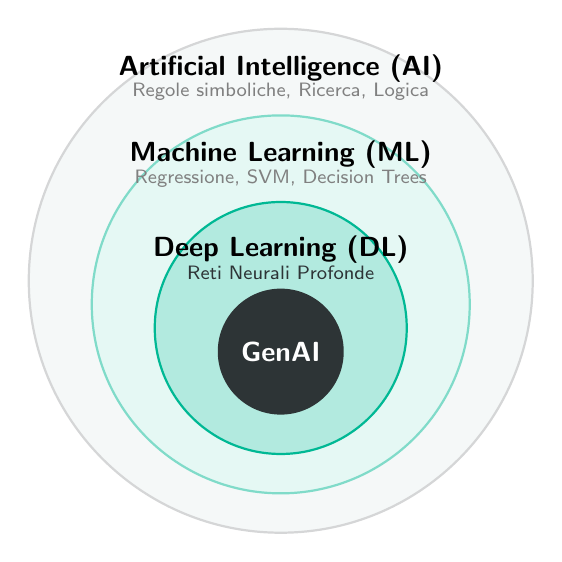
\begin{tikzpicture}
        % Circles
        \fill[Light!30] (0,0) circle (3.2);
        \draw[Dark!20, thick] (0,0) circle (3.2);
        \node at (0, 2.7) {\textbf{Artificial Intelligence (AI)}};
        \node[font=\scriptsize, color=gray] at (0, 2.4) {Regole simboliche, Ricerca, Logica};

        \fill[Accent!10] (0,-0.3) circle (2.4);
        \draw[Accent!50, thick] (0,-0.3) circle (2.4);
        \node at (0, 1.6) {\textbf{Machine Learning (ML)}};
        \node[font=\scriptsize, color=gray] at (0, 1.3) {Regressione, SVM, Decision Trees};

        \fill[Accent!30] (0,-0.6) circle (1.6);
        \draw[Accent, thick] (0,-0.6) circle (1.6);
        \node at (0, 0.4) {\textbf{Deep Learning (DL)}};
        \node[font=\scriptsize, color=Dark] at (0, 0.1) {Reti Neurali Profonde};
        
        \fill[Dark] (0,-0.9) circle (0.8);
        \node[text=White] at (0,-0.9) {\textbf{GenAI}};
    \end{tikzpicture}
    
    \vspace{0.5em}
    \flushleft\scriptsize
    \textbf{Nota}: Il Deep Learning è un tipo di ML che apprende \textbf{rappresentazioni} dei dati. La Generative AI è un sottoinsieme che \emph{crea} nuovi dati invece di classificarli.
\end{frame}

% --- SLIDE 4: What is ML ---
\begin{frame}{Che cos'è il Machine Learning?}
    \begin{block}{Definizione (Mitchell, 1997)}
        Si dice che un programma apprende dall'esperienza E con riferimento a alcune classi di compiti T e con misurazione della performance P, se le sue performance nel compito T, come misurato da P, migliorano con l'esperienza E.
    \end{block}

    \vspace{1em}
    \centering
    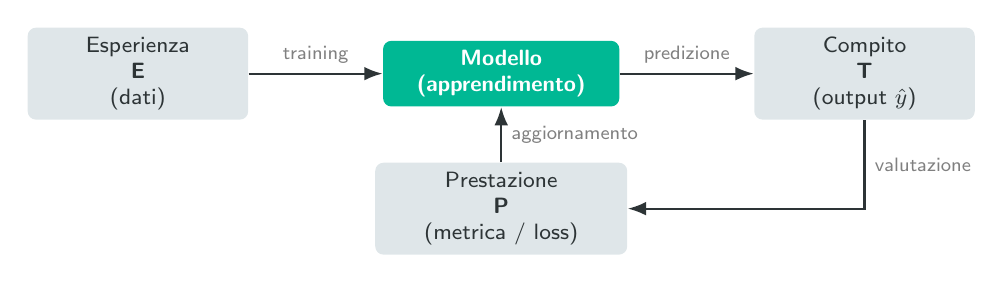
\begin{tikzpicture}[node distance=1.7cm]
        \node[flatnode, minimum width=2.8cm] (exp) {Esperienza\\\textbf{E}\\(dati)};
        \node[accentnode, right=of exp, minimum width=3.0cm] (model) {Modello\\(apprendimento)};
        \node[flatnode, right=of model, minimum width=2.8cm] (task) {Compito\\\textbf{T}\\(output $\hat{y}$)};
        \node[flatnode, below=0.7cm of model, minimum width=3.2cm] (perf) {Prestazione\\\textbf{P}\\(metrica / loss)};

        \draw[arrow] (exp) -- node[above, font=\scriptsize, color=gray] {training} (model);
        \draw[arrow] (model) -- node[above, font=\scriptsize, color=gray] {predizione} (task);
        \draw[arrow] (task.south) |- node[pos=0.25, right, font=\scriptsize, color=gray] {valutazione} (perf.east);
        \draw[arrow] (perf.north) -- node[right, font=\scriptsize, color=gray] {aggiornamento} (model.south);
    \end{tikzpicture}
    
    \vspace{0.5em}
    \small Invece di programmare le regole ("if-then"), programmiamo l'algoritmo per \emph{trovare} le regole dai dati.
\end{frame}

% --- SLIDE 5: What is DL ---
\begin{frame}{Che cos'è il Deep Learning? (Representation Learning)}
    \begin{columns}[T]
        \begin{column}{0.6\textwidth}
            \begin{itemize}
                \item \textbf{Problema del ML classico}: Richiede \emph{feature engineering} manuale (es. definire i bordi per riconoscere un volto).
                \item \textbf{Soluzione DL}: Apprende le feature automaticamente componendo rappresentazioni semplici in complesse.
                \item \textbf{"Deep"}: Si riferisce al numero di livelli (strati) nel grafo computazionale.
            \end{itemize}
        \end{column}
        \begin{column}{0.4\textwidth}
            \centering
            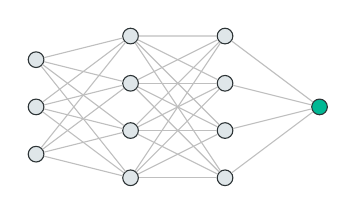
\begin{tikzpicture}[scale=0.6, transform shape]
                \foreach \y in {1,2,3} \node[circle,fill=Light,draw=Dark] (i\y) at (0,\y) {};
                \foreach \y in {1,...,4} \node[circle,fill=Light,draw=Dark] (h1\y) at (2,\y-0.5) {};
                \foreach \y in {1,...,4} \node[circle,fill=Light,draw=Dark] (h2\y) at (4,\y-0.5) {};
                \node[circle,fill=Accent,draw=Dark] (o) at (6,2) {};
                
                \foreach \s in {1,2,3} \foreach \d in {1,...,4} \draw[gray!50] (i\s) -- (h1\d);
                \foreach \s in {1,...,4} \foreach \d in {1,...,4} \draw[gray!50] (h1\s) -- (h2\d);
                \foreach \s in {1,...,4} \draw[gray!50] (h2\s) -- (o);
            \end{tikzpicture}
            \scriptsize\\Input $\to$ Features $\to$ Concetti $\to$ Output
        \end{column}
    \end{columns}
\end{frame}

% --- SLIDE 6: GenAI (Layout Fix: Compact & Scaled) ---
\begin{frame}{Che cos'è la Generative AI?}

    % Uso [c] (centered) invece di [T] per bilanciare meglio verticalmente se il testo è breve
    % Se preferisci l'allineamento in alto, rimetti [T]
    \begin{columns}[c] 

        % --- COLONNA SINISTRA: CONCETTI ---
        \begin{column}{0.45\textwidth}
            % Rimosso vspace eccessivo
            \begin{block}{AI Classica (Discriminativa)}
                \scriptsize % Testo leggermente più piccolo per sicurezza
                Lavora con categorie definite (\textbf{Discreto}).
                \begin{itemize}
                    \item \textbf{Obiettivo:} Etichettare/Classificare.
                    \item \textbf{Logica:} "O bianco, o nero". Confini netti.
                    \item \textit{Es: Spam (Sì/No).}
                \end{itemize}
            \end{block}

            \vspace{0.5em}

            \begin{block}{Generative AI}
                \scriptsize
                Lavora in uno spazio sfumato (\textbf{Continuo}).
                \begin{itemize}
                    \item \textbf{Obiettivo:} Creare nuove varianti.
                    \item \textbf{Logica:} "Sfumature infinite". Naviga per creare ibridi.
                    \item \textit{Es: Volti inesistenti.}
                \end{itemize}
            \end{block}
        \end{column}

        % --- COLONNA DESTRA: VISUALIZZAZIONE ---
        \begin{column}{0.5\textwidth}
            \centering
            
            % SCALA RIDOTTA A 0.68 PER STARE DENTRO I MARGINI
            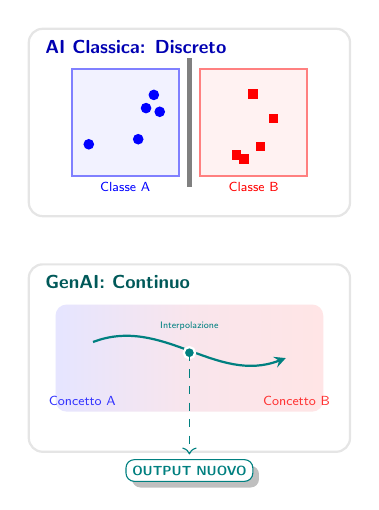
\begin{tikzpicture}[scale=0.68, transform shape]
                
                % Stili comuni
                \tikzset{
                    container/.style={rectangle, rounded corners=5pt, fill=white, draw=gray!20, thick,
                                     minimum width=6cm, minimum height=3.5cm}, % Larghezza fissa per uniformità
                    titlelabel/.style={font=\bfseries\normalsize, anchor=north west} % Font titolo leggibile
                }

                % --- 1. AI CLASSICA (Spostato coordinate per compattare) ---
                \node[container] (disc) at (0, 2.2) {}; % Y abbassata
                \node[titlelabel, text=blue!70!black] at ([xshift=0.2cm, yshift=-0.1cm]disc.north west) {AI Classica: Discreto};

                \begin{scope}[shift={(disc.center)}]
                    % Scatola A (Gatti)
                    \draw[thick, blue!50, fill=blue!5] (-2.2, -1) rectangle (-0.2, 1);
                    \node[below, font=\scriptsize, text=blue] at (-1.2, -1) {Classe A};
                    
                    % Scatola B (Cani)
                    \draw[thick, red!50, fill=red!5] (0.2, -1) rectangle (2.2, 1);
                    \node[below, font=\scriptsize, text=red] at (1.2, -1) {Classe B};

                    % Dati separati
                    \foreach \i in {1,...,5} \node[circle, fill=blue, inner sep=2pt] at ({-1.2 + rand*0.7}, {rand*0.7}) {};
                    \foreach \i in {1,...,5} \node[rectangle, fill=red, inner sep=2.5pt] at ({1.2 + rand*0.7}, {rand*0.7}) {};
                    
                    % Muro divisorio
                    \draw[ultra thick, gray] (0, -1.2) -- (0, 1.2);
                \end{scope}


                % --- 2. GEN AI (Spostato coordinate per compattare) ---
                \node[container] (gen) at (0, -2.2) {}; % Y alzata (ridotto gap tra i grafici)
                \node[titlelabel, text=teal!70!black] at ([xshift=0.2cm, yshift=-0.1cm]gen.north west) {GenAI: Continuo};

                \begin{scope}[shift={(gen.center)}]
                    
                    % Spazio Latente
                    \shade[left color=blue!10, right color=red!10, middle color=purple!10, rounded corners=4pt] 
                        (-2.5, -1) rectangle (2.5, 1);
                    
                    % Etichette poli
                    \node[font=\scriptsize, text=blue!80] at (-2, -0.8) {Concetto A};
                    \node[font=\scriptsize, text=red!80] at (2, -0.8) {Concetto B};

                    % Traiettoria
                    \draw[thick, teal, ->, >=stealth] (-1.8, 0.3) .. controls (-0.5, 0.8) and (0.5, -0.5) .. (1.8, 0);
                    \node[font=\tiny, text=teal, above] at (0, 0.4) {Interpolazione};

                    % Punto selezionato
                    \fill[teal, draw=white, thick] (0, 0.1) circle (3pt);
                    \draw[->, teal, dashed] (0, 0.1) -- (0, -1.8);

                    % Output Box che esce leggermente dal container per effetto 3D
                    \node[draw=teal, fill=white, rounded corners=3pt, font=\scriptsize\bfseries, text=teal, drop shadow] at (0, -2.1) {OUTPUT NUOVO};
                    
                \end{scope}

            \end{tikzpicture}
        \end{column}

    \end{columns}
\end{frame}

% --- SLIDE 7: Historical Trends ---
\begin{frame}{Historical Trends: Le Tre Ondate (Goodfellow, Ch. 1.2)}
    \begin{enumerate}
        \item \textbf{Cibernetica (1940-1960)}:
        \begin{itemize}
            \item Modelli ispirati biologicamente (McCulloch-Pitts, Perceptron).
            \item Limite: Incapacità di apprendere funzioni non lineari (XOR problem).
        \end{itemize}
        \item \textbf{Connessionismo (1980-1995)}:
        \begin{itemize}
            \item Backpropagation, Distributed Representation.
            \item Reti neurali (LSTM, CNN iniziali).
            \item Declino dovuto ai Kernel Methods (SVM) che erano più facili da allenare.
        \end{itemize}
        \item \textbf{Deep Learning (2006-Oggi)}:
        \begin{itemize}
            \item Convergenza di: \textbf{Big Data}, \textbf{GPU} e tecniche di training migliori (ReLU, Dropout, pre-training).
        \end{itemize}
    \end{enumerate}
\end{frame}

% --- SLIDE 8: Timeline ---
\begin{frame}{Timeline dell'AI}
    \centering
    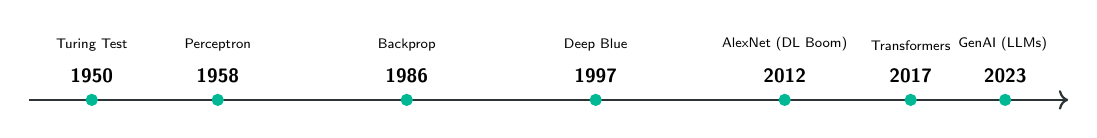
\begin{tikzpicture}[x=0.8cm, y=1cm]
        \draw[->, thick, Dark] (0,0) -- (16.5,0);
        
        % Ticks
        \foreach \x/\y/\t/\desc in {
            1/1950/below/Turing Test,
            3/1958/above/Perceptron,
            6/1986/below/Backprop,
            9/1997/above/Deep Blue,
            12/2012/below/AlexNet (DL Boom),
            14/2017/above/Transformers,
            15.5/2023/below/GenAI (LLMs)
        } {
            \draw[Accent, fill=Accent] (\x,0) circle (2pt);
            \node[font=\scriptsize\bfseries] at (\x, 0.3) {\y};
            \ifx\t\below
                \node[font=\tiny, align=center, anchor=north] at (\x, -0.2) {\desc};
            \else
                \node[font=\tiny, align=center, anchor=south] at (\x, 0.5) {\desc};
            \fi
        }
    \end{tikzpicture}
\end{frame}

% --- SLIDE 9: Types of Learning ---
\begin{frame}{Types of Learning: Panoramica}
    \centering
    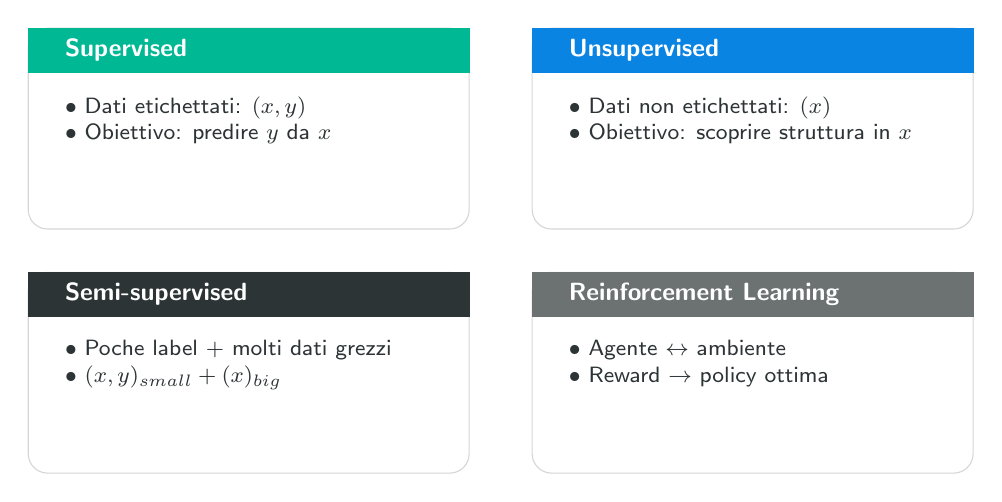
\begin{tikzpicture}[x=1cm, y=1cm]
        % --- Card base style (local to this picture) ---
        \tikzset{
            card/.style={draw=Dark!20, rounded corners=7pt, fill=White, minimum width=5.6cm, minimum height=2.55cm},
            bar/.style={rounded corners=7pt},
        }

        % --- Layout (2x2 grid) ---
        \node[card] (sup)  at (-3.2,  1.55) {};
        \node[card] (uns)  at ( 3.2,  1.55) {};
        \node[card] (semi) at (-3.2, -1.55) {};
        \node[card] (rl)   at ( 3.2, -1.55) {};

        % Header bars
        \fill[Accent]    ([yshift=0pt]sup.north west)  rectangle ([yshift=-0.58cm]sup.north east);
        \fill[Secondary] ([yshift=0pt]uns.north west)  rectangle ([yshift=-0.58cm]uns.north east);
        \fill[Dark]      ([yshift=0pt]semi.north west) rectangle ([yshift=-0.58cm]semi.north east);
        \fill[Dark!70]   ([yshift=0pt]rl.north west)   rectangle ([yshift=-0.58cm]rl.north east);

        % Icons (simple) + titles
        \node[anchor=west, font=\bfseries\small, text=White] at ([xshift=0.35cm,yshift=-0.29cm]sup.north west) {Supervised};
        \node[anchor=west, font=\bfseries\small, text=White] at ([xshift=0.35cm,yshift=-0.29cm]uns.north west) {Unsupervised};
        \node[anchor=west, font=\bfseries\small, text=White] at ([xshift=0.35cm,yshift=-0.29cm]semi.north west) {Semi-supervised};
        \node[anchor=west, font=\bfseries\small, text=White] at ([xshift=0.35cm,yshift=-0.29cm]rl.north west) {Reinforcement Learning};

        % Body text
        \node[align=left, font=\footnotesize, text=Dark, anchor=north west] at ([xshift=0.35cm,yshift=-0.75cm]sup.north west) {$\bullet$ Dati etichettati: $(x, y)$\\$\bullet$ Obiettivo: predire $y$ da $x$};

        \node[align=left, font=\footnotesize, text=Dark, anchor=north west] at ([xshift=0.35cm,yshift=-0.75cm]uns.north west) {$\bullet$ Dati non etichettati: $(x)$\\$\bullet$ Obiettivo: scoprire struttura in $x$};

        \node[align=left, font=\footnotesize, text=Dark, anchor=north west] at ([xshift=0.35cm,yshift=-0.75cm]semi.north west) {$\bullet$ Poche label + molti dati grezzi\\$\bullet$ $(x, y)_{small} + (x)_{big}$};

        \node[align=left, font=\footnotesize, text=Dark, anchor=north west] at ([xshift=0.35cm,yshift=-0.75cm]rl.north west) {$\bullet$ Agente $\leftrightarrow$ ambiente\\$\bullet$ Reward $\to$ policy ottima};
    \end{tikzpicture}
\end{frame}

% --- SLIDE 10: Supervised Learning (Visual) ---
\begin{frame}{Supervised Learning (Il "cavallo di battaglia")}
    \begin{columns}[T]
        % --- COLONNA SINISTRA: TEORIA ---
        \begin{column}{0.55\textwidth}
            \vspace{0.5em}
            \begin{itemize}
                \item \textbf{Input}: Dataset etichettato
                \[ \mathcal{D} = \{(\mathbf{x}_1, y_1), \dots, (\mathbf{x}_n, y_n)\} \]
                \item \textbf{Obiettivo}: Trovare la funzione $f$ tale che:
                \[ f(\mathbf{x}) \approx y \]
                per fare predizioni su nuovi dati.
            \end{itemize}
            
            \vspace{1em}
            \textbf{Esempi Reali:}
            \begin{itemize}
                \item \textcolor{Accent}{\textbf{Regressione}}: Predire il prezzo di una casa (continuo).
                \item \textcolor{Secondary}{\textbf{Classificazione}}: Diagnosticare una malattia (sano/malato).
            \end{itemize}
        \end{column}

        % --- COLONNA DESTRA: GRAFICI ---
        \begin{column}{0.45\textwidth}
            \centering
            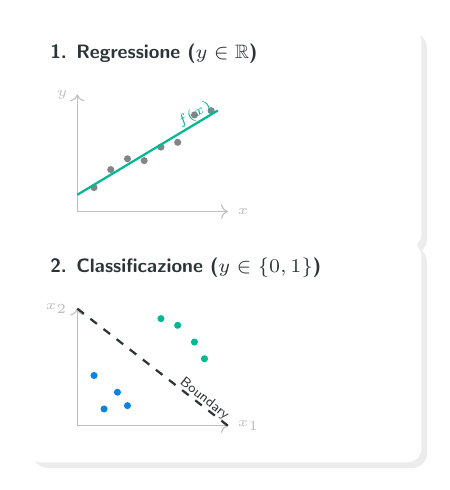
\begin{tikzpicture}[scale=0.85]
                % Stile Card
                \tikzset{
                    plotcard/.style={
                        rectangle, fill=White, rounded corners=5pt, 
                        minimum width=5cm, minimum height=2.8cm,
                        drop shadow={opacity=0.15, shadow xshift=2pt, shadow yshift=-2pt}
                    }
                }

                % --- 1. REGRESSION CARD ---
                \node[plotcard] (reg) at (0, 3.2) {};
                
                % Titolo Card
                \node[anchor=north west, font=\bfseries\scriptsize, text=Dark] at ([xshift=0.2cm, yshift=-0.1cm]reg.north west) {1. Regressione ($y \in \mathbb{R}$)};
                
                % Grafico Regressione
                \begin{scope}[shift={([xshift=-2.2cm, yshift=-1.1cm]reg.center)}, scale=0.5]
                    \draw[->, gray!50] (0,0) -- (4.5,0) node[right, font=\tiny] {$x$};
                    \draw[->, gray!50] (0,0) -- (0,3.5) node[left, font=\tiny] {$y$};
                    
                    % Punti (noisy)
                    \foreach \x in {0.5, 1.0, 1.5, 2.0, 2.5, 3.0, 3.5, 4.0}
                        \fill[Dark!60] (\x, {0.6*\x + 0.5 + rand*0.4}) circle (3pt);
                        
                    % Modello (Retta)
                    \draw[thick, Accent] (0, 0.5) -- (4.2, 3.02);
                    \node[Accent, font=\tiny, rotate=30] at (3.5, 2.9) {$f(x)$};
                \end{scope}

                % --- 2. CLASSIFICATION CARD ---
                \node[plotcard] (cls) at (0, 0) {};
                
                % Titolo Card
                \node[anchor=north west, font=\bfseries\scriptsize, text=Dark] at ([xshift=0.2cm, yshift=-0.1cm]cls.north west) {2. Classificazione ($y \in \{0, 1\}$)};
                
                % Grafico Classificazione
                \begin{scope}[shift={([xshift=-2.2cm, yshift=-1.1cm]cls.center)}, scale=0.5]
                    \draw[->, gray!50] (0,0) -- (4.5,0) node[right, font=\tiny] {$x_1$};
                    \draw[->, gray!50] (0,0) -- (0,3.5) node[left, font=\tiny] {$x_2$};
                    
                    % Classe 0 (Blu)
                    \foreach \p in {(0.8,0.5), (1.2,1.0), (0.5,1.5), (1.5, 0.6)}
                        \fill[Secondary] \p circle (3pt);
                        
                    % Classe 1 (Verde/Accent)
                    \foreach \p in {(3.0,3.0), (3.5,2.5), (2.5,3.2), (3.8, 2.0)}
                        \fill[Accent] \p circle (3pt);
                        
                    % Decision Boundary
                    \draw[thick, Dark, dashed] (0, 3.5) -- (4.5, 0);
                    \node[Dark, font=\tiny, rotate=-38] at (3.8, 0.8) {Boundary};
                \end{scope}

            \end{tikzpicture}
        \end{column}
    \end{columns}
\end{frame}

% --- SLIDE 11: Unsupervised Learning (Visual) ---
\begin{frame}{Unsupervised Learning (Scoperta di conoscenza)}
    \begin{columns}[T]
        % --- COLONNA SINISTRA: TEORIA ---
        \begin{column}{0.55\textwidth}
            \vspace{0.5em}
            \begin{itemize}
                \item \textbf{Input}: Dataset non etichettato
                \[ \mathcal{D} = \{\mathbf{x}_1, \dots, \mathbf{x}_n\} \]
                \item \textbf{Obiettivo}: Apprendere la \textbf{struttura} nascosta o la distribuzione $p(\mathbf{x})$.
            \end{itemize}
            
            \vspace{1em}
            \textbf{Task Principali:}
            \begin{itemize}
                \item \textcolor{Secondary}{\textbf{Clustering}}: Raggruppare dati simili (es. segmentazione clienti).
                \item \textcolor{Accent}{\textbf{Dim. Reduction}}: Comprimere le informazioni mantenendo la varianza (es. compressione immagini).
                \item \textbf{Density Est.}: Rilevare anomalie.
            \end{itemize}
        \end{column}

        % --- COLONNA DESTRA: GRAFICI ---
        \begin{column}{0.45\textwidth}
            \centering
            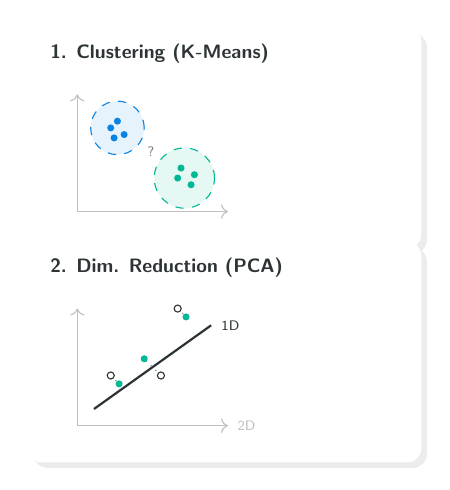
\begin{tikzpicture}[scale=0.85]
                % Stile Card (uguale alla slide precedente)
                \tikzset{
                    plotcard/.style={
                        rectangle, fill=White, rounded corners=5pt, 
                        minimum width=5cm, minimum height=2.8cm,
                        drop shadow={opacity=0.15, shadow xshift=2pt, shadow yshift=-2pt}
                    }
                }

                % --- 1. CLUSTERING CARD ---
                \node[plotcard] (clus) at (0, 3.2) {};
                
                % Titolo
                \node[anchor=north west, font=\bfseries\scriptsize, text=Dark] at ([xshift=0.2cm, yshift=-0.1cm]clus.north west) {1. Clustering (K-Means)};
                
                % Grafico
                \begin{scope}[shift={([xshift=-2.2cm, yshift=-1.1cm]clus.center)}, scale=0.5]
                    \draw[->, gray!50] (0,0) -- (4.5,0);
                    \draw[->, gray!50] (0,0) -- (0,3.5);
                    
                    % Cluster 1
                    \draw[dashed, Secondary, fill=Secondary!10] (1.2, 2.5) circle (0.8cm);
                    \foreach \p in {(1.0,2.5), (1.4,2.3), (1.2,2.7), (1.1, 2.2)}
                        \fill[Secondary] \p circle (3pt);
                        
                    % Cluster 2
                    \draw[dashed, Accent, fill=Accent!10] (3.2, 1.0) circle (0.9cm);
                    \foreach \p in {(3.0,1.0), (3.4,0.8), (3.1,1.3), (3.5, 1.1)}
                        \fill[Accent] \p circle (3pt);
                        
                    \node[font=\tiny, gray] at (2.2, 1.8) {?};
                \end{scope}

                % --- 2. DIMENSIONALITY REDUCTION CARD ---
                \node[plotcard] (dim) at (0, 0) {};
                
                % Titolo
                \node[anchor=north west, font=\bfseries\scriptsize, text=Dark] at ([xshift=0.2cm, yshift=-0.1cm]dim.north west) {2. Dim. Reduction (PCA)};
                
                % Grafico
                \begin{scope}[shift={([xshift=-2.2cm, yshift=-1.1cm]dim.center)}, scale=0.5]
                    \draw[->, gray!50] (0,0) -- (4.5,0) node[right, font=\tiny] {2D};
                    \draw[->, gray!50] (0,0) -- (0,3.5);
                    
                    % Principal Component Line
                    \draw[thick, Dark] (0.5, 0.5) -- (4.0, 3.0) node[right, font=\tiny] {1D};
                    
                    % Points projecting
                    \coordinate (p1) at (1.0, 1.5); \coordinate (proj1) at (1.25, 1.25);
                    \coordinate (p2) at (2.5, 1.5); \coordinate (proj2) at (2.0, 2.0);
                    \coordinate (p3) at (3.0, 3.5); \coordinate (proj3) at (3.25, 3.25);
                    
                    % Draw projection lines
                    \draw[dotted, gray] (p1) -- (proj1);
                    \draw[dotted, gray] (p2) -- (proj2);
                    \draw[dotted, gray] (p3) -- (proj3);
                    
                    % Original points (Hollow)
                    \foreach \p in {p1, p2, p3} \draw[Dark, fill=white] (\p) circle (3pt);
                    
                    % Projected points (Solid)
                    \foreach \p in {proj1, proj2, proj3} \fill[Accent] (\p) circle (3pt);
                    
                \end{scope}

            \end{tikzpicture}
        \end{column}
    \end{columns}
\end{frame}

% --- SLIDE 12: Semi-supervised Learning (Re-styled & New Visual) ---
\begin{frame}{Semi-supervised Learning: Sfruttare la struttura}
    \begin{columns}[T]
        % --- COLONNA SINISTRA: TEORIA ---
        \begin{column}{0.55\textwidth}
            \vspace{0.5em}
            \begin{itemize}
                \item \textbf{Problema Reale}:
                \begin{itemize}
                    \item Dati etichettati ($L$): Costosi, rari.
                    \item Dati non etichettati ($U$): Economici, abbondanti.
                \end{itemize}
                \item \textbf{Intuizione Chiave}:
                I dati non etichettati ci mostrano la \textbf{forma} (la distribuzione sottostante) dei dati.
                \item \textbf{Come funziona}:
                Le etichette dei pochi punti $L$ vengono "propagate" ai punti $U$ vicini, seguendo le zone ad alta densità.
            \end{itemize}
            \vspace{0.5em}
            \begin{alertblock}{Manifold Assumption}
                Punti vicini nello spazio delle feature ad alta densità probabilmente hanno la stessa etichetta.
            \end{alertblock}
        \end{column}

        % --- COLONNA DESTRA: GRAFICI (STILE PLOTCARD) ---
        \begin{column}{0.45\textwidth}
            \centering
            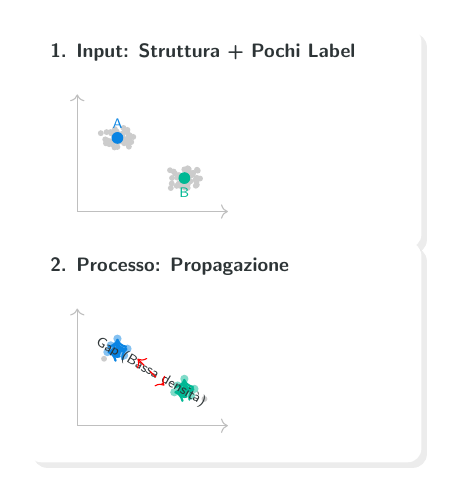
\begin{tikzpicture}[scale=0.85]
                % Stile Card (Preso dalla slide di riferimento)
                \tikzset{
                    plotcard/.style={
                        rectangle, fill=White, rounded corners=5pt, 
                        minimum width=5cm, minimum height=2.8cm,
                        drop shadow={opacity=0.15, shadow xshift=2pt, shadow yshift=-2pt}
                    }
                }

                % --- CARD 1: INPUT (Pochi Labeled, Molti Unlabeled) ---
                \node[plotcard] (input) at (0, 3.2) {};
                
                % Titolo
                \node[anchor=north west, font=\bfseries\scriptsize, text=Dark] at ([xshift=0.2cm, yshift=-0.1cm]input.north west) {1. Input: Struttura + Pochi Label};
                
                % Grafico
                \begin{scope}[shift={([xshift=-2.2cm, yshift=-1.1cm]input.center)}, scale=0.5]
                    %\draw[help lines] (0,0) grid (4.5, 3.5); % Debug
                    \draw[->, gray!50] (0,0) -- (4.5,0);
                    \draw[->, gray!50] (0,0) -- (0,3.5);
                    
                    % --- Struttura dati (Due "lune" o cluster densi) ---
                    % Cluster Sinistro (Unlabeled - Grigio)
                    \foreach \x in {0.8, 1.0, 1.2, 1.4, 1.6, 1.1, 1.3, 1.5} {
                        \foreach \y in {2.0, 2.2, 2.4, 2.1, 2.3} {
                             \fill[gray!40] (\x + rand*0.1, \y + rand*0.1) circle (2.5pt);
                        }
                    }
                    
                    % Cluster Destro (Unlabeled - Grigio)
                    \foreach \x in {2.8, 3.0, 3.2, 3.4, 3.6, 3.1, 3.3, 3.5} {
                        \foreach \y in {0.8, 1.0, 1.2, 0.9, 1.1} {
                             \fill[gray!40] (\x + rand*0.1, \y + rand*0.1) circle (2.5pt);
                        }
                    }
                    
                    % --- Punti Labeled (Solo UNO per cluster) ---
                    % Label Classe A (Secondary/Blu) nel cluster sinistro
                    \fill[Secondary] (1.2, 2.2) circle (5pt) node[above, font=\tiny, Secondary] {A};
                    
                    % Label Classe B (Accent/Verde) nel cluster destro
                    \fill[Accent] (3.2, 1.0) circle (5pt) node[below, font=\tiny, Accent] {B};
                    
                \end{scope}

                % --- CARD 2: PROCESSO (Label Propagation) ---
                \node[plotcard] (prop) at (0, 0) {};
                
                % Titolo
                \node[anchor=north west, font=\bfseries\scriptsize, text=Dark] at ([xshift=0.2cm, yshift=-0.1cm]prop.north west) {2. Processo: Propagazione};
                
                % Grafico
                \begin{scope}[shift={([xshift=-2.2cm, yshift=-1.1cm]prop.center)}, scale=0.5]
                    \draw[->, gray!50] (0,0) -- (4.5,0);
                    \draw[->, gray!50] (0,0) -- (0,3.5);

                    % --- Ripeto i punti originali ---
                    \fill[Secondary] (1.2, 2.2) circle (5pt);
                    \fill[Accent] (3.2, 1.0) circle (5pt);

                    % --- Propagazione Classe A (Sinistra) ---
                    % Punti vicini si colorano (Secondary leggero)
                    \foreach \p in {(1.0, 2.4), (1.4, 2.1), (1.2, 2.6), (0.9, 2.2), (1.5, 2.3)}
                        \fill[Secondary!50] \p circle (3.5pt);
                    % Frecce di flusso
                    \draw[->, thick, Secondary] (1.2, 2.2) -- (0.9, 2.2);
                    \draw[->, thick, Secondary] (1.2, 2.2) -- (1.5, 2.3);
                    \draw[->, thick, Secondary] (1.2, 2.2) -- (1.2, 2.6);

                    % --- Propagazione Classe B (Destra) ---
                    % Punti vicini si colorano (Accent leggero)
                    \foreach \p in {(3.0, 1.2), (3.4, 0.9), (3.2, 1.4), (2.9, 1.0), (3.5, 1.1)}
                        \fill[Accent!50] \p circle (3.5pt);
                    % Frecce di flusso
                    \draw[->, thick, Accent] (3.2, 1.0) -- (2.9, 1.0);
                    \draw[->, thick, Accent] (3.2, 1.0) -- (3.5, 1.1);
                    \draw[->, thick, Accent] (3.2, 1.0) -- (3.2, 1.4);
                    
                    % --- Punti lontani rimangono grigi (per ora) ---
                    \fill[gray!40] (0.8, 2.0) circle (2.5pt);
                    \fill[gray!40] (3.8, 0.8) circle (2.5pt);

                    % --- Gap tra i cluster ---
                    \node[font=\tiny, Dark, rotate=-30] at (2.2, 1.6) {Gap (Bassa densità)};
                    \draw[<->, red, dashed] (1.8, 2.0) -- (2.6, 1.2);

                \end{scope}

            \end{tikzpicture}
        \end{column}
    \end{columns}
\end{frame}

% --- SLIDE 13: Reinforcement Learning ---
\begin{frame}{Reinforcement Learning (Cenni)}
    Non c'è un supervisore che dà la risposta corretta, ma un segnale di \textbf{Reward} (spesso ritardato).
    
    \vspace{1em}
    \centering
    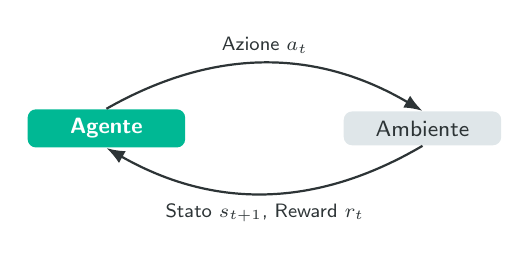
\begin{tikzpicture}[node distance=2cm]
        \node[accentnode, minimum width=2cm] (agent) {Agente};
        \node[flatnode, right=of agent, minimum width=2cm] (env) {Ambiente};
        
        \draw[arrow, bend left] (agent.north) to node[above, font=\scriptsize] {Azione $a_t$} (env.north);
        \draw[arrow, bend left] (env.south) to node[below, font=\scriptsize] {Stato $s_{t+1}$, Reward $r_t$} (agent.south);
    \end{tikzpicture}
    
    \vspace{1em}
    \flushleft
    \textbf{Sfida}: Trade-off tra \emph{Exploration} (provare cose nuove) ed \emph{Exploitation} (usare ciò che funziona).
\end{frame}

% --- SLIDE 14: How Supervised Learning Works (Exploded Formula) ---
\begin{frame}{Come funziona il Supervised Learning?}

    % Introduzione testuale (mantenuta ma compattata)
    \small
    Il processo fondamentale in 3 passi:
    \begin{enumerate}
        \item \textbf{Rappresentazione}: Trasformare il mondo reale (audio, pixel) in un vettore numerico $\mathbf{x}$ (Feature Vector).
        \item \textbf{Valutazione (Loss Function)}: Definire una funzione di costo $\mathcal{L}(f(\mathbf{x}), y)$ che misura l'errore (es. distanza quadratica, cross-entropy).
        \item \textbf{Ottimizzazione}: Modificare i parametri $\theta$ del modello per minimizzare la Loss media sul training set.
    \end{enumerate}

    \vspace{-0.2em}

    % --- VISUALIZZAZIONE DELLA FORMULA ---
    \centering
    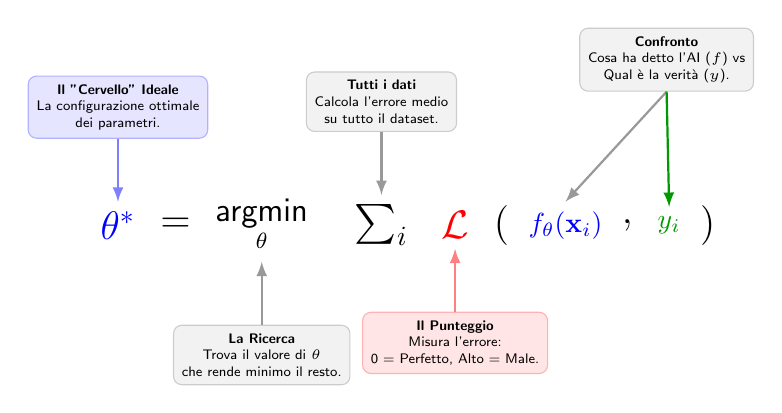
\begin{tikzpicture}[
        scale=1, transform shape,
        % Stile per i box di spiegazione
        note/.style={
            rectangle, rounded corners=3pt, fill=gray!10, draw=gray!40,
            font=\tiny\sffamily, align=center, inner sep=3pt
        },
        % Stile per le frecce
        arr/.style={->, >=latex, gray!80, thick}
    ]

        % 1. Costruiamo la formula pezzo per pezzo per poterla puntare
        % Theta Star (Il risultato finale)
        \node[font=\Large\bfseries, text=blue] (theta_star) at (0,0) {$\theta^*$};
        
        \node[right=2pt of theta_star, font=\Large] (eq) {$=$};
        
        % Argmin (L'operazione di ricerca)
        \node[right=2pt of eq, font=\large] (argmin) {$\underset{\theta}{\text{argmin}}$};
        
        % Somma (Il ciclo sui dati)
        \node[right=10pt of argmin, font=\Large] (sum) {$\sum_{i}$};
        
        % Loss Function (Il cuore del problema)
        \node[right=5pt of sum, font=\Large\bfseries, text=red] (loss) {$\mathcal{L}$};
        
        % Parentesi aperta
        \node[right=2pt of loss, font=\Large] (par_open) {$($};
        
        % Predizione (f di x)
        \node[right=0pt of par_open, font=\normalsize, text=blue] (pred) {$f_\theta(\mathbf{x}_i)$};
        
        % Virgola
        \node[right=0pt of pred, font=\Large] (comma) {$,$};
        
        % Verità (y)
        \node[right=2pt of comma, font=\normalsize, text=green!60!black] (truth) {$y_i$};
        
        % Parentesi chiusa
        \node[right=0pt of truth, font=\Large] (par_close) {$)$};


        % --- 2. Aggiungiamo le annotazioni (Frecce e Spiegazioni) ---

        % Spiegazione Theta Star (Sopra)
        \node[note, above=0.8cm of theta_star, fill=blue!10, draw=blue!30] (note_theta) 
            {\textbf{Il "Cervello" Ideale}\\La configurazione ottimale\\dei parametri.};
        \draw[arr, blue!50] (note_theta) -- (theta_star);

        % Spiegazione Argmin (Sotto)
        \node[note, below=0.8cm of argmin] (note_argmin) 
            {\textbf{La Ricerca}\\Trova il valore di $\theta$\\che rende minimo il resto.};
        \draw[arr] (note_argmin) -- (argmin);

        % Spiegazione Somma (Sopra - leggermente a destra)
        \node[note, above=0.8cm of sum] (note_sum) 
            {\textbf{Tutti i dati}\\Calcola l'errore medio\\su tutto il dataset.};
        \draw[arr] (note_sum) -- (sum);

        % Spiegazione Loss (Sotto)
        \node[note, below=0.8cm of loss, fill=red!10, draw=red!30] (note_loss) 
            {\textbf{Il Punteggio}\\Misura l'errore:\\0 = Perfetto, Alto = Male.};
        \draw[arr, red!50] (note_loss) -- (loss);

        % Spiegazione Predizione vs Realtà (Sopra unificata)
        \node[note, above=1.5cm of comma, xshift=0.5cm] (note_diff) 
            {\textbf{Confronto}\\Cosa ha detto l'AI ($f$) vs\\Qual è la verità ($y$).};
        
        % Frecce che partono dallo stesso box e vanno ai due elementi
        \draw[arr] (note_diff.south) -- (pred.north);
        \draw[arr, green!60!black] (note_diff.south) -- (truth.north);

    \end{tikzpicture}

    \vspace{0.5em}
    \centering
    \textit{\footnotesize "Cerchiamo i parametri ($\theta$) che rendono minima la somma degli errori ($\mathcal{L}$) tra le previsioni e la realtà."}

\end{frame}

% --- SLIDE 15: Why it works (Generalization) ---
\begin{frame}{Perché funziona su nuovi dati? (Generalizzazione)}
    \begin{alertblock}{Ipotesi I.I.D.}
        I dati di training e di test sono \textbf{Indipendenti} e \textbf{Identicamente Distribuiti}, campionati dalla stessa distribuzione generatrice $P_{data}$.
    \end{alertblock}
    
    \begin{itemize}
        \item \textbf{Underfitting}: Il modello è troppo semplice per catturare la struttura (High Bias).
        \item \textbf{Overfitting}: Il modello memorizza il rumore del training set (High Variance).
        \item L'obiettivo non è minimizzare l'errore di training, ma l'errore di \textbf{generalizzazione} (test).
    \end{itemize}
\end{frame}

% ==============================================================================
% SEZIONE 2: IL TOOLBOX MATEMATICO
% ==============================================================================

% --- MODULE TITLE SLIDE ---
\begin{frame}[plain]
    \centering
    \vspace{2cm}
    {\Huge \textbf{Modulo 2}}\\[0.5cm]
    {\Huge \textcolor{Accent}{Il Toolbox Matematico}}\\[1cm]
    {\large Algebra Lineare, Probabilità e Ottimizzazione}
\end{frame}

\section{2. Matematica per il ML: Algebra e Probabilità}

% --- SLIDE 16: Algebra Lineare ---
\begin{frame}{Algebra Lineare: Il "Motore" del ML}
    \begin{columns}
        \begin{column}{0.6\textwidth}
            Perché è fondamentale?
            \begin{itemize}
                \item \textbf{Rappresentazione}: I dati sono vettori, le immagini sono matrici, i video sono tensori.
                \item \textbf{Efficienza}: Le operazioni vettoriali sono parallelizzabili su GPU.
                \item \textbf{Concetti Core}: Norme (errore), Autovalori (importanza delle feature), SVD (compressione).
            \end{itemize}
        \end{column}
        \begin{column}{0.4\textwidth}
            \centering
            \[ \mathbf{y} = \sigma(\mathbf{W}\mathbf{x} + \mathbf{b}) \]
            \small L'equazione base di una rete neurale è pura algebra lineare.
        \end{column}
    \end{columns}
\end{frame}

% --- SLIDE 17: Scalars & Vectors (Professional Layout) ---
\begin{frame}{Notazione: Scalari e Vettori}

    \begin{columns}[T,onlytextwidth]
        % --- COLONNA SINISTRA: TESTO ---
        \begin{column}{0.5\textwidth}
            \vspace{0.2em} % Spazio dall'alto
            \begin{block}{\textbf{1. Scalare} ($x \in \mathbb{R}$)}
                \small Un singolo numero. Indica solo una quantità (es. prezzo, temperatura).
            \end{block}

            \vspace{0.8em}

            \begin{block}{\textbf{2. Vettore} ($\mathbf{x} \in \mathbb{R}^n$)}
                \scriptsize Una lista ordinata di numeri.
                \[ \mathbf{x} = \begin{bmatrix} x_1 \\ x_2 \end{bmatrix} \]
                In geometria, un vettore è definito da 3 proprietà:
                \begin{itemize}
                    \item \textbf{Modulo}: Lunghezza (intensità).
                    \item \textbf{Direzione}: La retta su cui giace.
                    \item \textbf{Verso}: Dove punta la freccia.
                \end{itemize}
            \end{block}
        \end{column}

        % --- COLONNA DESTRA: GRAFICI ---
        \begin{column}{0.5\textwidth}
            \centering
            
            % SCALARE (Pulito e semplice)
            
\begin{tikzpicture}[scale=0.8, transform shape]
                \node[anchor=west, font=\bfseries] at (-2.5, 0.5) {Scalare:};
                \draw[thick, gray!80, -{Stealth[length=2mm]}] (-2,0) -- (3,0); 
                \foreach \x in {-1,0,1,2} \draw[gray!80] (\x,-0.1) -- (\x,0.1);
                \fill[blue] (1.5,0) circle (3pt);
                \node[blue, above, font=\scriptsize] at (1.5,0.1) {$x=1.5$};
                \node[right, gray, font=\tiny] at (3,0) {Solo grandezza};
            \end{tikzpicture}

            \vspace{1.8em}

            % VETTORE (Grafico di alta qualità)
            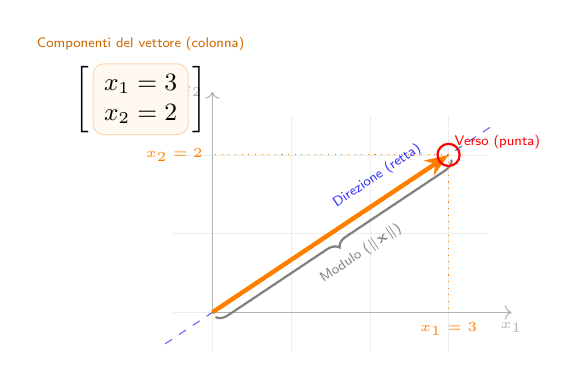
\begin{tikzpicture}[scale=1.0, transform shape]
                % Definizioni
                \coordinate (O) at (0,0);
                \coordinate (P) at (3,2);
                
                % Assi e Griglia
                \draw[gray!15, very thin] (-0.5,-0.5) grid (3.5,2.5);
                \draw[->, gray!60] (O) -- (3.8,0) node[below, font=\tiny] {$x_1$};
                \draw[->, gray!60] (O) -- (0,2.8) node[left, font=\tiny] {$x_2$};

                % 1. DIREZIONE (linea di fondo)
                \draw[dashed, thin, blue!60] ($(O)!-0.2!(P)$) -- ($(O)!1.2!(P)$);
                \node[blue!80, font=\tiny, rotate=34, anchor=south, yshift=2pt] at ($(O)!0.75!(P)$) {Direzione (retta)};

                % 2. MODULO (parentesi graffa)
                \draw[decoration={brace, mirror, amplitude=4pt, raise=2pt}, decorate, thick, gray] 
                     (O) -- (P);
                \node[gray, font=\tiny, rotate=34, anchor=north, yshift=-6pt] at ($(O)!0.55!(P)$) {Modulo ($\|\mathbf{x}\|$)};

                % 3. VETTORE (freccia principale)
                \draw[->, ultra thick, orange, -{Stealth[length=3mm]}] (O) -- (P);
                
                % 4. VERSO (cerchio sulla punta)
                \draw[red, thick] (P) circle (4pt);
                \node[red, font=\tiny, anchor=south west, inner sep=2pt] at (P) {Verso (punta)};

                % Proiezioni e Matrice Dati
                \draw[dotted, orange] (P) -- (P |- O) node[below, font=\tiny] {$x_1=3$};
                \draw[dotted, orange] (P) -- (P -| O) node[left, font=\tiny] {$x_2=2$};
                
                \node[matrix of math nodes, left delimiter={[}, right delimiter={]}, 
                      fill=orange!5, draw=orange!30, rounded corners, inner sep=2pt,
                      anchor=south east, font=\small] (vec_matrix) at (-0.3, 2.25) { x_1=3 \\ x_2=2 \\ };
                \node[above=1pt of vec_matrix, font=\tiny, color=orange!80!black] {Componenti del vettore (colonna)};
            \end{tikzpicture}
        \end{column}
    \end{columns}
\end{frame}

% --- SLIDE: Matrici e Tensori (Definitions) ---
\begin{frame}{Matrici e Tensori: Oltre i Vettori}
    \begin{columns}[T,onlytextwidth]
        % --- COLONNA 1: MATRICI ---
        \begin{column}{0.48\textwidth}
            \begin{block}{1. La Matrice ($\mathbb{R}^{m \times n}$)}
                \footnotesize
                Una tabella bidimensionale di numeri.
                \begin{itemize}
                    \item \textbf{Struttura}: Righe ($m$) $\times$ Colonne ($n$).
                    \item \textbf{Uso}: Dataset tabulari, immagini in bianco e nero, trasformazioni lineari (rotazioni, scalature).
                \end{itemize}
            \end{block}
            
            \vspace{0.3em}
            \centering
            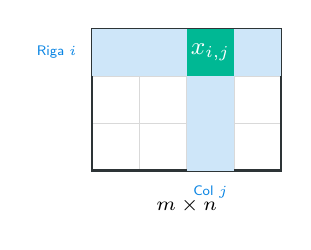
\begin{tikzpicture}[scale=0.75]
                % Griglia Matrice
                \draw[step=0.8, gray!30, thin] (0,0) grid (3.2, 2.4);
                \draw[thick, Dark] (0,0) rectangle (3.2, 2.4);
                
                % Evidenzia una riga (Vettore riga)
                \fill[Secondary!20] (0, 1.6) rectangle (3.2, 2.4);
                \node[font=\tiny, Secondary, anchor=east] at (-0.1, 2.0) {Riga $i$};
                
                % Evidenzia una colonna (Vettore colonna)
                \fill[Secondary!20] (1.6, 0) rectangle (2.4, 2.4);
                \node[font=\tiny, Secondary, anchor=north] at (2.0, -0.1) {Col $j$};
                
                % Cella incrocio (Elemento)
                \fill[Accent] (1.6, 1.6) rectangle (2.4, 2.4);
                \node[font=\small\bfseries, white] at (2.0, 2.0) {$x_{i,j}$};
                
                % Label dimensione
                \node[font=\scriptsize] at (1.6, -0.6) {$m \times n$};
            \end{tikzpicture}
        \end{column}

        % --- COLONNA 2: TENSORI ---
        \begin{column}{0.48\textwidth}
            \begin{block}{2. Il Tensore ($\mathbb{R}^{d_1 \times \dots \times d_k}$)}
                \footnotesize
                Generalizzazione a $k$ dimensioni (3D o più).
                \begin{itemize}
                    \item \textbf{Struttura}: Una matrice con "profondità" (Canali).
                    \item \textbf{Esempio Classico}: Immagine RGB.
                    \item È la struttura dati base di PyTorch/TensorFlow.
                \end{itemize}
            \end{block}
            
            \vspace{0.3em}
            \centering
            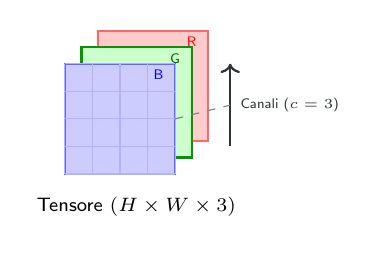
\begin{tikzpicture}[scale=0.70]
                % Layer Rosso (Red Channel) - Dietro
                \fill[red!20, draw=red!60, thick] (0.6, 0.6) rectangle (2.6, 2.6);
                \node[font=\tiny, red] at (2.3, 2.4) {R};
                
                % Layer Verde (Green Channel) - Centro
                \fill[green!20, draw=green!60!black, thick] (0.3, 0.3) rectangle (2.3, 2.3);
                \node[font=\tiny, green!40!black] at (2.0, 2.1) {G};
                
                % Layer Blu (Blue Channel) - Davanti
                \fill[blue!20, draw=blue!60, thick] (0, 0) rectangle (2, 2);
                \node[font=\tiny, blue] at (1.7, 1.8) {B};
                
                % Grid decorativa sul layer frontale
                \draw[step=0.5, blue!30, thin] (0,0) grid (2,2);
                
                % Linea di profondità
                \draw[->, thick, Dark] (3.0, 0.5) -- (3.0, 2.0) node[midway, right, font=\tiny] {Canali ($c=3$)};
                \draw[dashed, gray] (2.0, 1.0) -- (3.0, 1.25); % Linea guida
                
                % Descrizione
                \node[font=\scriptsize] at (1.3, -0.6) {Tensore $(H \times W \times 3)$};
            \end{tikzpicture}
        \end{column}
    \end{columns}
\end{frame}

% --- SLIDE: Data Representation (1D, 2D, 3D) ---
\begin{frame}{Rappresentazione dei Dati: Dai Vettori ai Tensori}
    \small
    Prima di calcolare, dobbiamo capire come il computer "vede" i dati.
    \vspace{0.5em}
    
    \begin{columns}[T]
        % --- 1D: VETTORE ---
        \begin{column}{0.33\textwidth}
            \centering
            \textbf{\textcolor{Secondary}{1D: Vettore}}
            \vspace{0.2cm}
            
            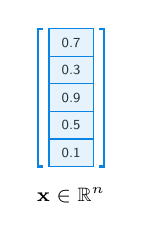
\begin{tikzpicture}[scale=0.7]
                % Strip verticale
                \foreach \y/\v in {0/0.1, 0.5/0.5, 1.0/0.9, 1.5/0.3, 2.0/0.7} {
                    \draw[fill=Secondary!10, draw=Secondary] (0,\y) rectangle (0.8,\y+0.5);
                    \node[font=\tiny, text=Dark] at (0.4, \y+0.25) {\v};
                }
                % Parentesi
                \draw[thick, Secondary] (-0.1, 0) -- (-0.2, 0) -- (-0.2, 2.5) -- (-0.1, 2.5);
                \draw[thick, Secondary] (0.9, 0) -- (1.0, 0) -- (1.0, 2.5) -- (0.9, 2.5);
                
                % Etichetta
                \node[below, font=\scriptsize, align=center] at (0.4, -0.2) {$\mathbf{x} \in \mathbb{R}^n$};
            \end{tikzpicture}
            
            \vspace{0.2cm}
            \scriptsize
            \textit{"Una lista di numeri"}\\
            \textbf{Esempi}:\\
            - Audio (onda sonora)\\
            - Caratteristiche casa (mq, stanze)
        \end{column}

        % --- 2D: MATRICE ---
        \begin{column}{0.33\textwidth}
            \centering
            \textbf{\textcolor{Dark}{2D: Matrice}}
            \vspace{0.2cm}
            
            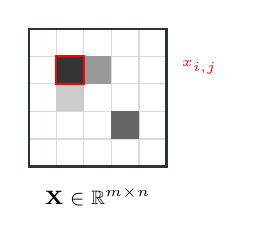
\begin{tikzpicture}[scale=0.7]
                % Griglia
                \draw[step=0.5, gray!30, thin] (0,0) grid (2.5, 2.5);
                \draw[thick, Dark] (0,0) rectangle (2.5, 2.5);
                
                % Pixel simulati (Greyscale)
                \fill[black!80] (0.5, 1.5) rectangle (1.0, 2.0);
                \fill[black!40] (1.0, 1.5) rectangle (1.5, 2.0);
                \fill[black!20] (0.5, 1.0) rectangle (1.0, 1.5);
                \fill[black!60] (1.5, 0.5) rectangle (2.0, 1.0);
                
                % Highlight un valore
                \draw[red, thick] (0.5, 1.5) rectangle (1.0, 2.0);
                \node[font=\tiny, red, anchor=west] at (2.6, 1.8) {$x_{i,j}$};
                
                % Etichetta
                \node[below, font=\scriptsize, align=center] at (1.25, -0.2) {$\mathbf{X} \in \mathbb{R}^{m \times n}$};
            \end{tikzpicture}
            
            \vspace{0.2cm}
            \scriptsize
            \textit{"Una tabella o griglia"}\\
            \textbf{Esempi}:\\
            - Dataset Excel\\
            - Immagine B/N
        \end{column}

        % --- 3D: TENSORE ---
        \begin{column}{0.33\textwidth}
            \centering
            \textbf{\textcolor{Accent}{3D: Tensore}}
            \vspace{0.2cm}
            
            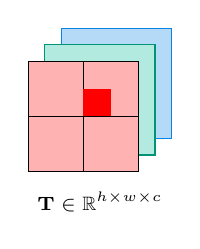
\begin{tikzpicture}[scale=0.7]
                % Layer 3 (Blue - Back)
                \fill[Secondary!30, draw=Secondary] (0.6, 0.6) rectangle (2.6, 2.6);
                
                % Layer 2 (Green - Middle)
                \fill[Accent!30, draw=Accent!80!black] (0.3, 0.3) rectangle (2.3, 2.3);
                
                % Layer 1 (Red - Front)
                \fill[red!30, draw=red] (0, 0) rectangle (2, 2);
                
                % Pixel frontale
                \draw[black, thin] (0,0) grid (2,2);
                \fill[red] (1,1) rectangle (1.5,1.5);
                
                % Etichetta
                \node[below, font=\scriptsize, align=center] at (1.3, -0.2) {$\mathbf{T} \in \mathbb{R}^{h \times w \times c}$};
            \end{tikzpicture}
            
            \vspace{0.2cm}
            \scriptsize
            \textit{"Un volume di dati"}\\
            \textbf{Esempi}:\\
            - Immagine a Colori (RGB)\\
            - Frame Video
        \end{column}
    \end{columns}
\end{frame}

% --- SLIDE 18: Sets & Notation (FIXED LAYOUT) ---
\begin{frame}{Notazione Insiemistica e Reali: Esempi Pratici}
    \small % Riduce il font globale per far stare tutto
    \begin{columns}[T]
        % --- COLONNA SINISTRA ---
        \begin{column}{0.5\textwidth}
            % Box 1: Insiemi
            \fcolorbox{Dark}{White}{
                \begin{minipage}{0.95\textwidth}
                    \raggedright
                    \textcolor{Dark}{\textbf{1. Insiemi ($\mathcal{S}, \mathcal{D}$)}}\\
                    \vspace{0.1cm}
                    \scriptsize
                    Collezione di elementi unici.
                    \begin{itemize}
                        \item \textbf{Esempio ML}: Classi possibili.
                        \[ \mathcal{Y} = \{\text{Gatto}, \text{Cane}, \text{Topo}\} \]
                        \item \textbf{Esempio Dataset}:
                        \[ \mathcal{D} = \{ (x_1, y_1), \dots, (x_m, y_m) \} \]
                    \end{itemize}
                    \vspace{0.1cm}
                \end{minipage}
            }
            \vspace{0.3cm} % Spazio tra i box

            % Box 2: Reali
            \fcolorbox{Dark}{White}{
                \begin{minipage}{0.95\textwidth}
                    \raggedright
                    \textcolor{Dark}{\textbf{2. Numeri Reali ($\mathbb{R}$)}}\\
                    \vspace{0.1cm}
                    \scriptsize
                    Spazio continuo.
                    \begin{itemize}
                        \item \textbf{Scalare} ($x \in \mathbb{R}$): Temperatura ($23.5^\circ$).
                        \item \textbf{Vettore} ($\mathbf{x} \in \mathbb{R}^3$): Una riga dati.
                        \[ \mathbf{x} = [180, 75, 30] \]
                    \end{itemize}
                    \vspace{0.1cm}
                \end{minipage}
            }
        \end{column}

        % --- COLONNA DESTRA ---
        \begin{column}{0.48\textwidth}
            % Box 3: Trasposta
            \fcolorbox{Dark}{White}{
                \begin{minipage}{0.95\textwidth}
                    \raggedright
                    \textcolor{Dark}{\textbf{3. Trasposta ($\mathbf{x}^\top$)}}\\
                    \vspace{0.1cm}
                    \scriptsize
                    Ruota i dati: righe $\leftrightarrow$ colonne.
                    \[
                    \mathbf{x} = \begin{bmatrix} 1 \\ 2 \\ 3 \end{bmatrix}
                    \xrightarrow{\text{T}}
                    \mathbf{x}^\top = \begin{bmatrix} 1 & 2 & 3 \end{bmatrix}
                    \]
                    \textit{Per allineare prima di moltiplicare.}
                    \vspace{0.1cm}
                \end{minipage}
            }
            \vspace{0.3cm}

            % Box 4: Indici
            \fcolorbox{Dark}{White}{
                \begin{minipage}{0.95\textwidth}
                    \raggedright
                    \textcolor{Dark}{\textbf{4. Indici di Matrice ($X_{i,j}$)}}\\
                    \vspace{0.1cm}
                    \scriptsize
                    Coordinate nella tabella.
                    \[
                    \mathbf{X} = 
                    \begin{bmatrix}
                    10 & \textcolor{Accent}{\mathbf{20}} \\
                    30 & 40
                    \end{bmatrix}
                    \]
                    \begin{itemize}
                        \item $i$ = Riga, $j$ = Colonna.
                        \item $X_{1,2} = \textcolor{Accent}{\mathbf{20}}$ (Riga 1, Col 2).
                    \end{itemize}
                    \vspace{0.1cm}
                \end{minipage}
            }
        \end{column}
    \end{columns}
\end{frame}

% --- SLIDE 19: Sum & Prod ---
\begin{frame}{Operatori Compatti ($\Sigma$ e $\Pi$)}
    Essenziali per scrivere le Loss Function.
    
    \begin{columns}[T]
        \begin{column}{0.5\textwidth}
            \textbf{Sommatoria ($\Sigma$)}
            \[ \sum_{i=1}^{n} x_i = x_1 + x_2 + \dots + x_n \]
            Esempio: Mean Squared Error (MSE).
        \end{column}
        \begin{column}{0.48\textwidth}
            \textbf{Produttoria ($\Pi$)}
            \[ \prod_{i=1}^{n} x_i = x_1 \cdot x_2 \cdot \dots \cdot x_n \]
            Esempio: Likelihood di campioni indipendenti.
        \end{column}
    \end{columns}
\end{frame}

% --- SLIDE 20: Element-wise Operations ---
\begin{frame}{Operazioni Element-wise (Punto per Punto)}
    \begin{columns}[T]
        \begin{column}{0.55\textwidth}
            \small % Riduzione font globale per questa colonna
            \begin{block}{Definizione}
                Applicare un'operazione binaria (somma, prodotto, sottrazione) separatamente su ogni coppia di elementi corrispondenti.
                \[ \mathbf{z} = \mathbf{x} + \mathbf{y} \implies z_i = x_i + y_i \]
            \end{block}
            
            \vspace{0.2em}
            \textbf{Vincolo fondamentale}:
            I vettori devono avere la \textbf{stessa dimensione} (shape).
            
            \vspace{0.5em}
            \textbf{A cosa serve nel ML?}
            \begin{itemize}
                \setlength\itemsep{1pt}
                \item \textbf{Aggiornamento Pesi}: $w_{new} = w_{old} - \eta \cdot \text{gradiente}$ (sottrazione element-wise).
                \item \textbf{Immagini}: Aggiungere luminosità a un'immagine (sommare uno scalare a tutti i pixel).
            \end{itemize}
        \end{column}

        \begin{column}{0.45\textwidth}
            \centering
            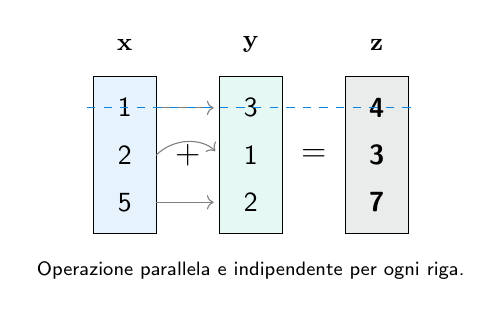
\begin{tikzpicture}[scale=0.8]
                % Vettore X
                \node[font=\bfseries\small] at (0, 3.5) {$\mathbf{x}$};
                \draw[fill=Secondary!10] (-0.5, 0.5) rectangle (0.5, 3.0);
                \node at (0, 2.5) {1};
                \node at (0, 1.75) {2};
                \node at (0, 1.0) {5};
                
                \node[font=\bfseries\large] at (1, 1.75) {$+$};
                
                % Vettore Y
                \node[font=\bfseries\small] at (2, 3.5) {$\mathbf{y}$};
                \draw[fill=Accent!10] (1.5, 0.5) rectangle (2.5, 3.0);
                \node at (2, 2.5) {3};
                \node at (2, 1.75) {1};
                \node at (2, 1.0) {2};
                
                \node[font=\bfseries\large] at (3, 1.75) {$=$};
                
                % Vettore Z
                \node[font=\bfseries\small] at (4, 3.5) {$\mathbf{z}$};
                \draw[fill=Dark!10] (3.5, 0.5) rectangle (4.5, 3.0);
                
                % Frecce
                % 1. Freccia Superiore (dritta)
                \draw[->, gray, shorten >=2pt] (0.5, 2.5) -- (1.5, 2.5); 
                \node[font=\bfseries] at (4, 2.5) {4};
                
                % 2. Freccia Centrale (CURVA per evitare il +)
                \draw[->, gray, shorten >=2pt] (0.5, 1.75) to[bend left=45] (1.5, 1.75); 
                \node[font=\bfseries] at (4, 1.75) {3};
                
                % 3. Freccia Inferiore (dritta)
                \draw[->, gray, shorten >=2pt] (0.5, 1.0) -- (1.5, 1.0); 
                \node[font=\bfseries] at (4, 1.0) {7};
                
                % Linea tratteggiata decorativa
                \draw[dashed, Secondary] (-0.6, 2.5) -- (4.6, 2.5);
                
                % TESTO INFERIORE (Inserito come nodo per evitare che vada a capo)
                % Posizionato a coordinate (2, 0), ovvero sotto i rettangoli
                \node[font=\scriptsize, anchor=north] at (2, 0.2) {Operazione parallela e indipendente per ogni riga.};
            \end{tikzpicture}
        \end{column}
    \end{columns}
\end{frame}

% --- SLIDE 20.1: Il Prodotto Scalare (Dot Product) ---
\begin{frame}{Il Mattoncino Base: Il Prodotto Scalare}
    \begin{columns}[T] % Allineamento in alto per evitare spazi strani
        
        % --- COLONNA TEORIA (Sinistra) ---
        \begin{column}{0.55\textwidth}
            \small % Font leggermente più piccolo per sicurezza
            
            \begin{block}{Definizione}
                Il \textbf{Prodotto Scalare} (o \textit{Dot Product}) è un'operazione tra due vettori della \textbf{stessa lunghezza}.
                Restituisce un \textbf{singolo numero} (scalare), non un vettore.
            \end{block}
            
            \vspace{0.5em}
            
            \onslide<2->{
                \textbf{Come funziona (Zip):}
                \begin{itemize}
                    \item Moltiplica il $1^{\circ}$ con il $1^{\circ}$, il $2^{\circ}$ con il $2^{\circ}$...
                    \item Somma i risultati.
                \end{itemize}
            }
            
            \vspace{0.5em}
            
            \onslide<3->{
                \textbf{Formula:}
                Dati $\mathbf{a}$ e $\mathbf{b}$ lunghi $N$:
                % Formula compattata per risparmiare spazio verticale
                \begin{align*}
                    \mathbf{a} \cdot \mathbf{b} &= \sum_{k=1}^{N} a_k \cdot b_k \\
                    &= (a_1 b_1) + \dots + (a_N b_N)
                \end{align*}
            }
        \end{column}

        % --- COLONNA VISUALIZZAZIONE (Destra) ---
        \begin{column}{0.45\textwidth}
            \centering
            % Scale ridotto leggermente per garantire i margini
            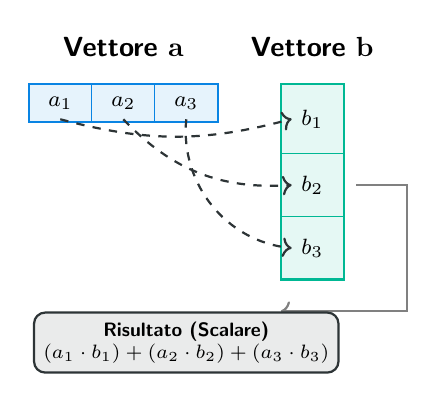
\begin{tikzpicture}[scale=0.8] 
                
                % --- Vettore RIGA (a) ---
                \node[font=\bfseries] at (1.5, 5.2) {Vettore $\mathbf{a}$};
                \draw[fill=Secondary!10, draw=Secondary, thick] (0, 4.0) rectangle (3, 4.6);
                \draw[Secondary] (1, 4.0) -- (1, 4.6);
                \draw[Secondary] (2, 4.0) -- (2, 4.6);
                
                % Etichette a
                \node[font=\footnotesize] (a1) at (0.5, 4.3) {$a_1$};
                \node[font=\footnotesize] (a2) at (1.5, 4.3) {$a_2$};
                \node[font=\footnotesize] (a3) at (2.5, 4.3) {$a_3$};

                % --- Vettore COLONNA (b) ---
                \node[font=\bfseries] at (4.5, 5.2) {Vettore $\mathbf{b}$};
                \draw[fill=Accent!10, draw=Accent, thick] (4.0, 1.5) rectangle (5.0, 4.6);
                \draw[Accent] (4.0, 2.5) -- (5.0, 2.5);
                \draw[Accent] (4.0, 3.5) -- (5.0, 3.5);
                
                % Etichette b
                \node[font=\footnotesize] (b1) at (4.5, 4.05) {$b_1$};
                \node[font=\footnotesize] (b2) at (4.5, 3.0) {$b_2$};
                \node[font=\footnotesize] (b3) at (4.5, 2.0) {$b_3$};

                % --- ANIMAZIONE 2: Collegamenti ---
                \onslide<2->{
                    % Frecce curve per mostrare l'accoppiamento senza incasinare il disegno
                    \draw[->, dashed, Dark, thick] (a1.south) to[bend right=15] (b1.west);
                    \draw[->, dashed, Dark, thick] (a2.south) to[bend right=25] (b2.west);
                    \draw[->, dashed, Dark, thick] (a3.south) to[bend right=45] (b3.west);
                }

                % --- ANIMAZIONE 3: Risultato ---
                \onslide<3->{
                    % Freccina che punta al risultato
                    \draw[->, thick, gray] (5.2, 3.0) -- (6.0, 3.0) -- (6.0, 1.0) -- (4.0, 1.0);
                    
                    % Box Risultato posizionato sotto i vettori
                    \node[draw=Dark, fill=Dark!10, thick, rounded corners, align=center, font=\scriptsize] at (2.5, 0.5) {
                        \textbf{Risultato (Scalare)} \\
                        $(a_1 \cdot b_1) + (a_2 \cdot b_2) + (a_3 \cdot b_3)$
                    };
                }

            \end{tikzpicture}
        \end{column}
    \end{columns}
\end{frame}

% --- SLIDE 20.2: Introduzione Moltiplicazione Matriciale (Animata) ---
\begin{frame}{Prodotto Matriciale (Righe $\times$ Colonne)}
    \begin{columns}[T]
        % --- COLONNA TESTO ---
        \begin{column}{0.55\textwidth}
            \small
            % 1. La regola appare subito
            \begin{block}{La Regola d'Oro}
                A differenza dell'element-wise, qui \textbf{non} accoppiamo elemento con elemento.
                
                Ogni cella del risultato è un \textbf{prodotto scalare} tra una \textbf{riga} della prima matrice e una \textbf{colonna} della seconda.
            \end{block}
            
            \vspace{0.8em}
            
            % 2. Le dimensioni appaiono al secondo step
            \onslide<2->{
                \textbf{1. Compatibilità Dimensioni}:
                Le colonne di A devono uguagliare le righe di B.
                \[ (M \times \textcolor{Secondary}{\mathbf{N}}) \cdot (\textcolor{Secondary}{\mathbf{N}} \times P) \to (M \times P) \]
            }
            
            \vspace{0.5em}
            
            % 3. La formula appare al terzo step (insieme alla riga nel grafico)
            \onslide<3->{
                \textbf{2. La Formula Generale}:
                L'elemento $(i, j)$ è dato da:
                \vspace{-0.3em} % Toglie un po' di spazio prima della formula
                \begin{align*}
                    C_{ij} &= \text{Riga}_i(A) \cdot \text{Col}_j(B) \\
                    &= \sum_{k=1}^{N} A_{ik} \cdot B_{kj}
                \end{align*}
            }
            
            % Riduco lo spazio prima della nota finale
            \vspace{0.2em} 
            
            \onslide<5->{
                \scriptsize \textit{Nota: Inner e Outer Product sono casi specifici!}
            }
        \end{column}

        % --- COLONNA GRAFICA ---
        \begin{column}{0.45\textwidth}
            \centering
            \vspace{0.5em}
            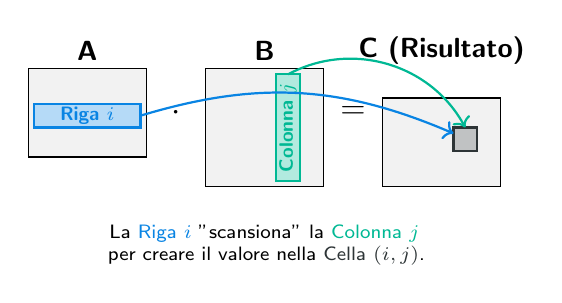
\begin{tikzpicture}[scale=0.75]
                % --- MATRICE A ---
                \node[font=\bfseries] at (1, 3.8) {A};
                \draw[fill=gray!10] (0, 2) rectangle (2, 3.5);
                
                % Animazione: La riga si illumina al click 3
                \draw<3->[fill=Secondary!30, draw=Secondary, thick] (0.1, 2.9) rectangle (1.9, 2.5);
                \node<3->[Secondary, font=\scriptsize\bfseries] at (1, 2.7) {Riga $i$};
                
                \node[font=\bfseries\large] at (2.5, 2.75) {$\cdot$};
                
                % --- MATRICE B ---
                \node[font=\bfseries] at (4, 3.8) {B};
                \draw[fill=gray!10] (3, 1.5) rectangle (5, 3.5);
                
                % Animazione: La colonna si illumina al click 4
                \draw<4->[fill=Accent!30, draw=Accent, thick] (4.2, 1.6) rectangle (4.6, 3.4);
                \node<4->[Accent, font=\scriptsize\bfseries, rotate=90] at (4.4, 2.5) {Colonna $j$};
                
                \node[font=\bfseries\large] at (5.5, 2.75) {$=$};
                
                % --- MATRICE C (RISULTATO) ---
                \node[font=\bfseries] at (7, 3.8) {C (Risultato)};
                \draw[fill=gray!10] (6, 1.5) rectangle (8, 3.0);
                
                % Animazione: La cella risultato si illumina al click 5
                \draw<5->[fill=Dark!30, draw=Dark, thick] (7.2, 2.1) rectangle (7.6, 2.5);
                
                % --- FRECCE ESPLICATIVE (Click 5) ---
                % Frecce che appaiono solo quando il calcolo è "completo"
                \draw<5->[->, Secondary, thick] (1.9, 2.7) to[bend left=20] (7.2, 2.4);
                \draw<5->[->, Accent, thick] (4.4, 3.4) to[bend left=45] (7.4, 2.5);
                
                % Annotazione sotto (Click 5)
                \node<5->[align=center, font=\scriptsize, text width=4cm] at (4, 0.5) {
                    La \textcolor{Secondary}{Riga $i$} "scansiona" la \textcolor{Accent}{Colonna $j$} per creare il valore nella \textcolor{Dark}{Cella $(i,j)$}.
                };
            \end{tikzpicture}
        \end{column}
    \end{columns}
\end{frame}

% --- SLIDE 20.3: Dot Product Definition ---
\begin{frame}{Prodotto Scalare: La Geometria}
    \begin{columns}[T]
        \begin{column}{0.5\textwidth}
            \begin{block}{Definizione Algebrica}
                Somma dei prodotti elemento per elemento. Restituisce un \textbf{singolo numero} (scalare).
                \[ \mathbf{x} \cdot \mathbf{y} = \sum_{i=1}^n x_i y_i \]
            \end{block}
            
            \begin{block}{Definizione Geometrica}
                \[ \mathbf{x} \cdot \mathbf{y} = \|\mathbf{x}\| \|\mathbf{y}\| \cos(\theta) \]
            \end{block}
            
            \small
            \textbf{Intuizione}:
            È la \textbf{proiezione} di un vettore sull'altro moltiplicata per la lunghezza. Ci dice quanto due frecce "spingono" nella stessa direzione.
        \end{column}

        \begin{column}{0.5\textwidth}
            \centering
            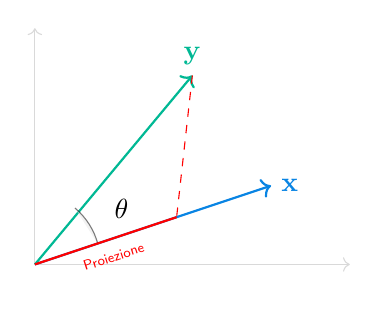
\begin{tikzpicture}[scale=2]
                % Assi
                \draw[->, gray!30] (0,0) -- (2,0);
                \draw[->, gray!30] (0,0) -- (0,1.5);
                
                % Vettori
                \draw[->, thick, Secondary] (0,0) -- (1.5, 0.5) node[right] {$\mathbf{x}$};
                \draw[->, thick, Accent] (0,0) -- (1.0, 1.2) node[above] {$\mathbf{y}$};
                
                % Angolo
                \draw[fill=gray!20, opacity=0.5] (0.4, 0.13) arc (15:50:0.45);
                \node at (0.55, 0.35) {$\theta$};
                
                % Proiezione
                \draw[dashed, red] (1.0, 1.2) -- (0.9, 0.3); % Proiezione perpendicolare approx
                \draw[thick, red] (0,0) -- (0.9, 0.3);
                \node[red, font=\tiny, rotate=18] at (0.5, 0.05) {Proiezione};
                
            \end{tikzpicture}
            
            \vspace{1em}
            \scriptsize
            Se $\theta = 90^\circ \implies \cos(90)=0 \implies$ Prodotto nullo.\\
            (I vettori sono \textbf{Ortogonali}/Indipendenti).
        \end{column}
    \end{columns}
\end{frame}

% --- SLIDE: Inner vs Outer Product ---
\begin{frame}{Attenzione all'ordine! Inner vs Outer Product}
    Date due colonne $\mathbf{u} = \begin{bmatrix}1\\3\end{bmatrix}$ e $\mathbf{v} = \begin{bmatrix}3\\1\end{bmatrix}$:
    \vspace{1em}
    
    \begin{columns}[T]
        % --- COLONNA 1: DOT PRODUCT (SCALARE) ---
        \begin{column}{0.48\textwidth}
            \centering
            \fcolorbox{Secondary}{White}{
                \begin{minipage}{0.95\textwidth}
                    \centering
                    \textbf{\textcolor{Secondary}{1. Inner Product (Dot)}}\\
                    \footnotesize (Riga $\times$ Colonna)
                    \vspace{0.5em}
                    
                    \[ \mathbf{u}^\top \mathbf{v} = \text{Scalare} \]
                    
                    \scriptsize
                    Regola dimensioni:
                    \[ (1 \times \mathbf{2}) \cdot (\mathbf{2} \times 1) \to (1 \times 1) \]
                    
                    \vspace{0.5em}
                    \textbf{Calcolo}:
                    \[
                    \begin{bmatrix} 1 & 3 \end{bmatrix} 
                    \cdot
                    \begin{bmatrix} 3 \\ 1 \end{bmatrix} 
                    \]
                    \[ = (1\cdot3) + (3\cdot1) = 3 + 3 = \mathbf{6} \]
                    
                    \vspace{0.5em}
                    \raggedright
                    \textit{Significato: "Quanto sono allineati i vettori?"}
                \end{minipage}
            }
        \end{column}

        % --- COLONNA 2: OUTER PRODUCT (MATRICE) ---
        \begin{column}{0.48\textwidth}
            \centering
            \fcolorbox{Accent}{White}{
                \begin{minipage}{0.95\textwidth}
                    \centering
                    \textbf{\textcolor{Accent}{2. Outer Product}}\\
                    \footnotesize (Colonna $\times$ Riga)
                    \vspace{0.5em}
                    
                    \[ \mathbf{u} \mathbf{v}^\top = \text{Matrice} \]
                    
                    \scriptsize
                    Regola dimensioni:
                    \[ (2 \times \mathbf{1}) \cdot (\mathbf{1} \times 2) \to (2 \times 2) \]
                    
                    \vspace{0.5em}
                    \textbf{Calcolo}:
                    \[
                    \begin{bmatrix} 1 \\ 3 \end{bmatrix} 
                    \cdot
                    \begin{bmatrix} 3 & 1 \end{bmatrix} 
                    =
                    \begin{bmatrix} 
                    1\cdot3 & 1\cdot1 \\
                    3\cdot3 & 3\cdot1
                    \end{bmatrix}
                    \]
                    \[ = \begin{bmatrix} 3 & 1 \\ 9 & 3 \end{bmatrix} \]
                    
                    \vspace{0.5em}
                    \raggedright
                    \textit{Significato: "Creare una griglia di tutte le interazioni".}
                \end{minipage}
            }
        \end{column}
    \end{columns}
\end{frame}

% --- SLIDE: Inner vs Outer Product (Real World Examples) ---
\begin{frame}{A cosa servono davvero? Esempi Visivi}
    \begin{columns}[T]
        % --- COLONNA 1: INNER PRODUCT (NETFLIX) ---
        \begin{column}{0.48\textwidth}
            \centering
            \fcolorbox{Secondary}{White}{
                \begin{minipage}{0.95\textwidth}
                    \centering
                    \textbf{\textcolor{Secondary}{Inner Product: Il "Match"}}
                    \vspace{0.3cm}
                    
                    \raggedright\scriptsize
                    \textbf{Obiettivo}: Ridurre a un solo numero (Score).
                    \textit{Esempio: Netflix Recommender.}
                    
                    \vspace{0.5em}
                    \centering
                    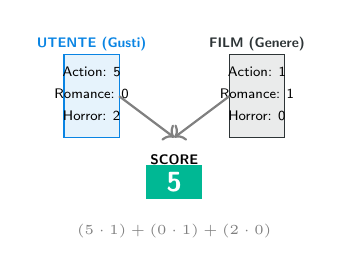
\begin{tikzpicture}[scale=0.7]
                        % Vettore Utente
                        \node[font=\bfseries\tiny, Secondary] at (0, 3.2) {UTENTE (Gusti)};
                        \draw[fill=Secondary!10, draw=Secondary] (-0.5, 1.5) rectangle (0.5, 3.0);
                        \node[font=\tiny] at (0, 2.7) {Action: 5};
                        \node[font=\tiny] at (0, 2.3) {Romance: 0};
                        \node[font=\tiny] at (0, 1.9) {Horror: 2};
                        
                        % Vettore Film
                        \node[font=\bfseries\tiny, Dark] at (3, 3.2) {FILM (Genere)};
                        \draw[fill=Dark!10, draw=Dark] (2.5, 1.5) rectangle (3.5, 3.0);
                        \node[font=\tiny] at (3, 2.7) {Action: 1};
                        \node[font=\tiny] at (3, 2.3) {Romance: 1};
                        \node[font=\tiny] at (3, 1.9) {Horror: 0};
                        
                        % Operazione
                        \draw[->, thick, gray] (0.5, 2.25) -- (1.5, 1.5);
                        \draw[->, thick, gray] (2.5, 2.25) -- (1.5, 1.5);
                        
                        % Risultato (Score)
                        \node[font=\bfseries\tiny] at (1.5, 1.1) {SCORE};
                        \draw[fill=Accent, draw=Accent] (1.0, 0.4) rectangle (2.0, 1.0);
                        \node[white, font=\bfseries] at (1.5, 0.7) {5}; 
                        
                        \node[font=\tiny, gray, align=center] at (1.5, -0.2) {$(5\cdot1) + (0\cdot1) + (2\cdot0)$};
                    \end{tikzpicture}
                    
                    \vspace{0.3cm}
                    \raggedright\scriptsize
                    \textbf{Risultato}: Uno scalare.\\
                    Il sistema ti consiglia il film se il numero è alto.
                \end{minipage}
            }
        \end{column}

        % --- COLONNA 2: OUTER PRODUCT (INTERACTION MAP) ---
        \begin{column}{0.48\textwidth}
            \centering
            \fcolorbox{Accent}{White}{
                \begin{minipage}{0.95\textwidth}
                    \centering
                    \textbf{\textcolor{Accent}{Outer Product: La "Griglia"}}
                    \vspace{0.3cm}
                    
                    \raggedright\scriptsize
                    \textbf{Obiettivo}: Creare una matrice di interazioni.
                    \textit{Esempio: Combinare Forme e Colori.}
                    
                    \vspace{0.5em}
                    \centering
                    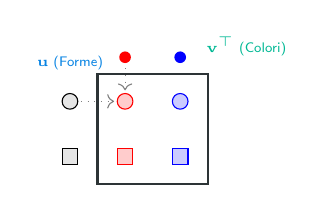
\begin{tikzpicture}[scale=0.7]
                        % Vettore Colonna (Forme)
                        \node[font=\tiny, anchor=south, Secondary] at (0.5, 2.6) {$\mathbf{u}$ (Forme)};
                        \node[draw, circle, inner sep=2pt, fill=gray!20] at (0.5, 2.2) {};
                        \node[draw, regular polygon, regular polygon sides=4, inner sep=2pt, fill=gray!20] at (0.5, 1.2) {};
                        
                        % Vettore Riga (Colori)
                        \node[font=\tiny, anchor=west, Accent] at (2.8, 3.2) {$\mathbf{v}^\top$ (Colori)};
                        \fill[red] (1.5, 3.0) circle (3pt);
                        \fill[blue] (2.5, 3.0) circle (3pt);
                        
                        % Matrice Risultante
                        \draw[thick, Dark] (1.0, 0.7) rectangle (3.0, 2.7);
                        
                        % Celle (Combinazioni)
                        % Cella 1,1 (Cerchio Rosso)
                        \node[draw, circle, inner sep=2pt, fill=red!20, draw=red] at (1.5, 2.2) {};
                        % Cella 1,2 (Cerchio Blu)
                        \node[draw, circle, inner sep=2pt, fill=blue!20, draw=blue] at (2.5, 2.2) {};
                        % Cella 2,1 (Quadrato Rosso)
                        \node[draw, regular polygon, regular polygon sides=4, inner sep=2pt, fill=red!20, draw=red] at (1.5, 1.2) {};
                        % Cella 2,2 (Quadrato Blu)
                        \node[draw, regular polygon, regular polygon sides=4, inner sep=2pt, fill=blue!20, draw=blue] at (2.5, 1.2) {};
                        
                        % Frecce indicative
                        \draw[->, gray, dotted] (0.7, 2.2) -- (1.3, 2.2);
                        \draw[->, gray, dotted] (1.5, 2.8) -- (1.5, 2.4);
                        
                    \end{tikzpicture}
                    
                    \vspace{0.3cm}
                    \raggedright\scriptsize
                    \textbf{Risultato}: Una matrice.\\
                    Ogni cella $(i,j)$ contiene la combinazione dell'elemento $u_i$ con $v_j$.
                \end{minipage}
            }
        \end{column}
    \end{columns}
    
    \vspace{0.5em}
    \centering
    \begin{alertblock}{In sintesi}
        \textbf{Inner} $\to$ Comprime (Analisi). \quad \textbf{Outer} $\to$ Espande (Sintesi).
    \end{alertblock}
\end{frame}

% --- SLIDE 1: Inner Product in ML ---
\begin{frame}{Inner Product nel Machine Learning: Il "Match"}
    \centering
    \textbf{Concetto}: Misurare la \textbf{compatibilità} tra due oggetti.
    \vspace{1em}

    \begin{columns}[T]
        \begin{column}{0.6\textwidth}
            \fcolorbox{Secondary}{White}{
                \begin{minipage}{0.95\textwidth}
                    \centering
                    \textbf{Esempio: Netflix / Spotify}
                    \vspace{0.5em}
                    
                    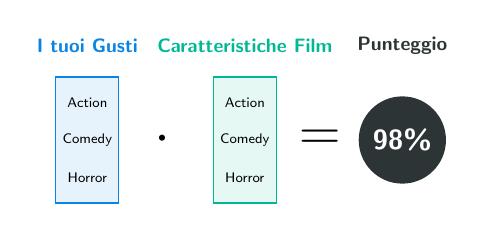
\begin{tikzpicture}[scale=0.8]
                        % Vettore Utente
                        \node[font=\bfseries\scriptsize, Secondary] at (0, 2.5) {I tuoi Gusti};
                        \draw[fill=Secondary!10, draw=Secondary] (-0.5, 0) rectangle (0.5, 2.0);
                        \node[font=\tiny] at (0, 1.6) {Action};
                        \node[font=\tiny] at (0, 1.0) {Comedy};
                        \node[font=\tiny] at (0, 0.4) {Horror};
                        
                        \node[font=\huge] at (1.2, 1) {$\cdot$};
                        
                        % Vettore Film
                        \node[font=\bfseries\scriptsize, Accent] at (2.5, 2.5) {Caratteristiche Film};
                        \draw[fill=Accent!10, draw=Accent] (2.0, 0) rectangle (3.0, 2.0);
                        \node[font=\tiny] at (2.5, 1.6) {Action};
                        \node[font=\tiny] at (2.5, 1.0) {Comedy};
                        \node[font=\tiny] at (2.5, 0.4) {Horror};
                        
                        \node[font=\huge] at (3.7, 1) {$=$};
                        
                        % Risultato
                        \node[font=\bfseries\scriptsize, Dark] at (5, 2.5) {Punteggio};
                        \node[circle, fill=Dark, text=white, minimum size=1cm] at (5, 1) {\textbf{98\%}};
                    \end{tikzpicture}
                \end{minipage}
            }
        \end{column}
        \begin{column}{0.4\textwidth}
            \small
            \vspace{1em}
            L'Inner Product "schiaccia" le due liste in un unico numero.
            \begin{itemize}
                \item Alto = \textbf{Compatibile}.
                \item Basso = \textbf{Da scartare}.
            \end{itemize}
        \end{column}
    \end{columns}
\end{frame}

% --- SLIDE 20.3: Dot Product as Similarity ---
\begin{frame}{Perché il Dot Product è il "cuore" del ML?}
    Nel Machine Learning usiamo il Dot Product per misurare la \textbf{Similarità}.
    \vspace{0.5em}
    
    \[ \text{Similarity}(\mathbf{x}, \mathbf{w}) \approx \mathbf{x}^\top \mathbf{w} \]
    
    \begin{columns}[T]
        \begin{column}{0.33\textwidth}
            \centering
            \fcolorbox{Accent}{White}{
                \begin{minipage}{0.9\textwidth}
                    \centering \scriptsize \textbf{Alta Similarità}\\
                    \vspace{0.2cm}
                    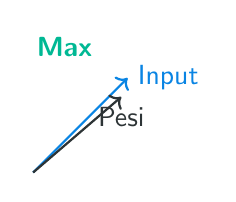
\begin{tikzpicture}[scale=0.8]
                        \draw[->, thick, Secondary] (0,0) -- (1.5, 1.5) node[right] {Input};
                        \draw[->, thick, Dark] (0,0) -- (1.4, 1.2) node[below] {Pesi};
                        \node[Accent, font=\bfseries] at (0.5, 2) {Max};
                    \end{tikzpicture}
                    \vspace{0.2cm}
                    I vettori sono allineati.\\Il neurone si "attiva".
                \end{minipage}
            }
        \end{column}
        
        \begin{column}{0.33\textwidth}
            \centering
            \fcolorbox{Secondary}{White}{
                \begin{minipage}{0.9\textwidth}
                    \centering \scriptsize \textbf{Nessuna Relazione}\\
                    \vspace{0.2cm}
                    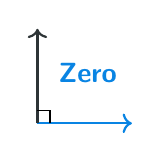
\begin{tikzpicture}[scale=0.8]
                        \draw[->, thick, Secondary] (0,0) -- (1.5, 0);
                        \draw[->, thick, Dark] (0,0) -- (0, 1.5);
                        \draw (0.2,0) |- (0,0.2);
                        \node[Secondary, font=\bfseries] at (0.8, 0.8) {Zero};
                    \end{tikzpicture}
                    \vspace{0.2cm}
                    Vettori Ortogonali.\\Il neurone ignora l'input.
                \end{minipage}
            }
        \end{column}
        
        \begin{column}{0.33\textwidth}
            \centering
            \fcolorbox{red}{White}{
                \begin{minipage}{0.9\textwidth}
                    \centering \scriptsize \textbf{Opposti}\\
                    \vspace{0.2cm}
                    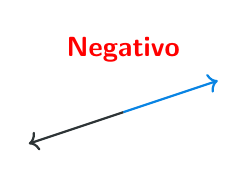
\begin{tikzpicture}[scale=0.8]
                        \draw[->, thick, Secondary] (0,0) -- (1.5, 0.5);
                        \draw[->, thick, Dark] (0,0) -- (-1.5, -0.5);
                        \node[red, font=\bfseries] at (0, 1) {Negativo};
                    \end{tikzpicture}
                    \vspace{0.2cm}
                    Disaccordo totale.\\Inibizione.
                \end{minipage}
            }
        \end{column}
    \end{columns}
    
    \vspace{1em}
    \textbf{Esempio Reale}: I "Recommender Systems" (Netflix) usano questo principio. Se il vettore \textit{Utente} è simile al vettore \textit{Film}, allora ti consiglia il film.
\end{frame}

% --- SLIDE 2: Inner Product in DL ---
\begin{frame}{Inner Product nel Deep Learning: L'Attivazione}
    \centering
    \textbf{Concetto}: Il neurone agisce come un \textbf{filtro} che cerca uno specifico pattern.
    \vspace{1em}

    \begin{columns}[T]
        \begin{column}{0.6\textwidth}
            \fcolorbox{Dark}{White}{
                \begin{minipage}{0.95\textwidth}
                    \centering
                    \textbf{Esempio: Riconoscere un Bordo}
                    \vspace{0.5em}
                    
                    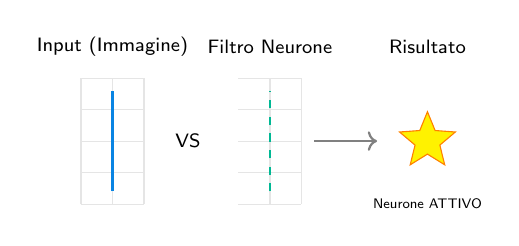
\begin{tikzpicture}[scale=0.8]
                        % Input (Immagine)
                        \node[font=\scriptsize] at (0, 2.5) {Input (Immagine)};
                        \draw[step=0.5, gray!20] (-0.5, 0) grid (0.5, 2);
                        \draw[thick, Secondary] (0, 0.2) -- (0, 1.8); % Linea verticale
                        
                        \node[font=\scriptsize] at (1.2, 1) {VS};
                        
                        % Peso (Filtro)
                        \node[font=\scriptsize] at (2.5, 2.5) {Filtro Neurone};
                        \draw[step=0.5, gray!20] (2.0, 0) grid (3.0, 2);
                        \draw[thick, Accent, dashed] (2.5, 0.2) -- (2.5, 1.8); % Cerca linea verticale
                        
                        \draw[->, thick, gray] (3.2, 1) -- (4.2, 1);
                        
                        % Output
                        \node[font=\scriptsize] at (5, 2.5) {Risultato};
                        \node[star, star points=5, star point ratio=2.25, fill=yellow, draw=orange] at (5, 1) {};
                        \node[font=\tiny] at (5, 0) {Neurone ATTIVO};
                    \end{tikzpicture}
                \end{minipage}
            }
        \end{column}
        \begin{column}{0.4\textwidth}
            \small
            \vspace{1em}
            Il neurone fa l'Inner Product tra l'immagine e il suo filtro interno.
            \begin{itemize}
                \item Se le forme coincidono $\to$ \textbf{Click!} (Si accende).
            \end{itemize}
        \end{column}
    \end{columns}
\end{frame}

% --- SLIDE 21: Matrices ---
\begin{frame}{Matrici e Tensori}
    \begin{itemize}
        \setlength{\itemsep}{0.4cm} 
        
        % Punto 1: Matrice
        \item 
        \begin{minipage}[c]{0.58\linewidth}
            \textbf{Matrice} ($\mathbf{A} \in \mathbb{R}^{m \times n}$): tabella bidimensionale. Rappresenta una \emph{trasformazione lineare} tra spazi.
        \end{minipage}
        \hfill
        \begin{minipage}[c]{0.38\linewidth}
            \centering
            $ \mathbf{A} = 
            \begin{bmatrix} 
                a_{11} & a_{12} & a_{13} \\ 
                a_{21} & a_{22} & a_{23} 
            \end{bmatrix} $
        \end{minipage}

        % Punto 2: Prodotto Matrice-Vettore
        \item 
        \begin{minipage}[c]{0.58\linewidth}
            \textbf{Prodotto matrice-vettore} ($\mathbf{b} = \mathbf{A}\mathbf{x}$): mappa il vettore $\mathbf{x}$ (da $n$ dimensioni) nel vettore $\mathbf{b}$ (a $m$ dimensioni) tramite \emph{combinazioni lineari} delle colonne di $\mathbf{A}$.
        \end{minipage}
        \hfill
        \begin{minipage}[c]{0.38\linewidth}
            \centering
            % \resizebox adatta l'equazione larga alla larghezza della colonna
            \resizebox{\linewidth}{!}{$
            \underbrace{\begin{bmatrix} 
                1 & 0 & -1 \\ 
                0 & 2 & 1 
            \end{bmatrix}}_{\mathbf{A}_{(2 \times 3)}}
            \underbrace{\begin{bmatrix} 
                2 \\ 
                1 \\ 
                3 
            \end{bmatrix}}_{\mathbf{x}_{(3 \times 1)}}
            =
            \underbrace{\begin{bmatrix} 
                1(2) + 0(1) - 1(3) \\ 
                0(2) + 2(1) + 1(3) 
            \end{bmatrix}}_{\text{Comb. lineare}}
            =
            \underbrace{\begin{bmatrix} 
                -1 \\ 
                5 
            \end{bmatrix}}_{\mathbf{b}_{(2 \times 1)}}
            $}
        \end{minipage}

        % Punto 3: Prodotto Matrice-Matrice
        \item 
        \begin{minipage}[c]{0.58\linewidth}
            \textbf{Prodotto matrice-matrice}: composizione di trasformazioni. Non commutativo ($\mathbf{AB} \neq \mathbf{BA}$).
        \end{minipage}
        \hfill
        \begin{minipage}[c]{0.38\linewidth}
            \centering
            $ \underset{(\color{blue}m \times \color{orange}k)}{\mathbf{A}} \cdot \underset{(\color{orange}k \times \color{blue}n)}{\mathbf{B}} = \underset{(\color{blue}m \times \color{blue}n)}{\mathbf{C}} $
        \end{minipage}

        % Punto 4: Tensore
        \item 
        \begin{minipage}[c]{0.58\linewidth}
            \textbf{Tensore}: generalizzazione a $n$ dimensioni (es. griglia 3D di pixel RGB).
        \end{minipage}
        \hfill
        \begin{minipage}[c]{0.38\linewidth}
            \centering
            \vspace{0.1cm}
            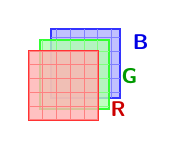
\begin{tikzpicture}[scale=0.35, every node/.style={transform shape}]
                % Livello Blu (Canale B)
                \draw[fill=blue!30, fill opacity=0.8, draw=blue!80, thick] (0.8,0.8) rectangle +(2.5,2.5);
                \draw[step=0.5, blue!50, very thin] (0.8,0.8) grid +(2.5,2.5);
                \node[anchor=west, text=blue!90!black, scale=2.2, font=\bfseries] at (3.5, 2.8) {B};
                
                % Livello Verde (Canale G)
                \draw[fill=green!30, fill opacity=0.8, draw=green!80, thick] (0.4,0.4) rectangle +(2.5,2.5);
                \draw[step=0.5, green!50, very thin] (0.4,0.4) grid +(2.5,2.5);
                \node[anchor=west, text=green!60!black, scale=2.2, font=\bfseries] at (3.1, 1.6) {G};
                
                % Livello Rosso (Canale R)
                \draw[fill=red!30, fill opacity=0.8, draw=red!80, thick] (0,0) rectangle +(2.5,2.5);
                \draw[step=0.5, red!50, very thin] (0,0) grid +(2.5,2.5);
                \node[anchor=west, text=red!80!black, scale=2.2, font=\bfseries] at (2.7, 0.4) {R};
            \end{tikzpicture}
        \end{minipage}

    \end{itemize}
\end{frame}


% --- SLIDE 21b: Geometria delle Matrici (Versione Professionale) ---
\begin{frame}{Lo Spazio Geometrico: Cosa fa davvero una Matrice?}
    \begin{columns}[T,onlytextwidth]
        \setlength{\columnsep}{0.25cm}
        \begin{column}{0.48\textwidth}
            \scriptsize
            Una matrice $\mathbf{A}$ applica una \textbf{trasformazione lineare} allo spazio. 
            
            \vspace{0.15cm}
            \textbf{La regola d'oro:} Le colonne di $\mathbf{A}$ sono le destinazioni finali dei vettori base $\hat{i}(1,0)$ e $\hat{j}(0,1)$.
            
            \vspace{0.1cm}
            \[
            \mathbf{A} = \begin{bmatrix} \color{orange}2 & \color{purple}-1 \\ \color{orange}1 & \color{purple}1 \end{bmatrix} \implies 
            \begin{cases} 
            \mathbf{A}\hat{i} = (\color{orange}2\color{black}, \color{orange}1\color{black}) \\ 
            \mathbf{A}\hat{j} = (\color{purple}-1\color{black}, \color{purple}1\color{black}) 
            \end{cases}
            \]
            \vspace{0.05cm}
            
            Prendiamo un vettore specifico $\mathbf{v} = \begin{bmatrix} 2 \\ 3 \end{bmatrix}$. \\
            Il prodotto canonico "righe per colonne" si scompone in una \textbf{combinazione lineare} delle colonne di $\mathbf{A}$:
            
            \vspace{0.05cm}
            \[
            \mathbf{A}\mathbf{v} = \begin{bmatrix} (\color{orange}2\color{black}\cdot 2) + (\color{purple}-1\color{black}\cdot 3) \\ (\color{orange}1\color{black}\cdot 2) + (\color{purple}1\color{black}\cdot 3) \end{bmatrix} =
            2 \begin{bmatrix} \color{orange}2 \\ \color{orange}1 \end{bmatrix} 
            + 3 \begin{bmatrix} \color{purple}-1 \\ \color{purple}1 \end{bmatrix} 
            \]
            \vspace{-0.1cm}
            \[
            = \begin{bmatrix} \color{orange}4 \\ \color{orange}2 \end{bmatrix} + \begin{bmatrix} \color{purple}-3 \\ \color{purple}3 \end{bmatrix} 
            = \begin{bmatrix} \color{blue}1 \\ \color{blue}5 \end{bmatrix}
            \]
            \vspace{0.05cm}
            
            \textit{\footnotesize Nel grafico: vedi il vettore v (grigio) trasformato in Av (blu) sommando i nuovi vettori base scalati.}
        \end{column}
        
        \begin{column}{0.50\textwidth}
            \centering
            \vspace{-0.2cm}
            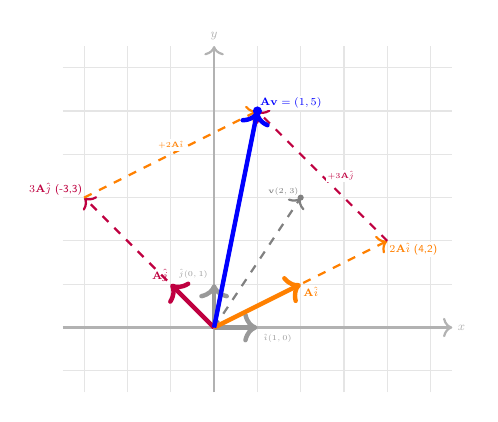
\begin{tikzpicture}[scale=0.55, transform shape]
                % Griglia e Assi
                \draw[step=1cm, gray!20, thin] (-3.5,-1.5) grid (5.5, 6.5);
                \draw[->, thick, gray!60] (-3.5,0) -- (5.5,0) node[right, font=\footnotesize] {$x$};
                \draw[->, thick, gray!60] (0,-1.5) -- (0,6.5) node[above, font=\footnotesize] {$y$};

                % Vettori base originali (Prima della trasformazione)
                \draw[->, ultra thick, black!40] (0,0) -- (1,0) node[below right, font=\tiny] {$\hat{i}(1,0)$};
                \draw[->, ultra thick, black!40] (0,0) -- (0,1) node[above left, font=\tiny] {$\hat{j}(0,1)$};
                
                % Vettore v originale (2,3) prima della trasformazione
                \draw[->, thick, gray, dashed] (0,0) -- (2,3) node[above left, font=\tiny, fill=white, inner sep=1pt] {$\mathbf{v}(2,3)$};
                \fill[gray] (2,3) circle (2pt);

                % Colonne di A (I nuovi assi base)
                \draw[->, ultra thick, orange] (0,0) -- (2,1) node[below right, font=\scriptsize, fill=white, inner sep=1pt] {$\mathbf{A}\hat{i}$};
                \draw[->, ultra thick, purple] (0,0) -- (-1,1) node[above left, font=\scriptsize, fill=white, inner sep=1pt] {$\mathbf{A}\hat{j}$};

                % Combinazione Lineare: Costruzione del Parallelogramma
                % Lato 1: 2 * Col1
                \draw[->, thick, orange, dashed] (0,0) -- (4,2) node[below right, font=\scriptsize, fill=white, inner sep=1pt] {$2\mathbf{A}\hat{i}$ (4,2)};
                % Lato 2: 3 * Col2
                \draw[->, thick, purple, dashed] (0,0) -- (-3,3) node[above left, font=\scriptsize, fill=white, inner sep=1pt] {$3\mathbf{A}\hat{j}$ (-3,3)};

                % Chiusura del parallelogramma (Mostra l'addizione vettoriale esatta)
                \draw[->, thick, purple, dashed] (4,2) -- (1,5) node[midway, right=2pt, font=\tiny, fill=white, inner sep=1pt] {$+3\mathbf{A}\hat{j}$};
                \draw[->, thick, orange, dashed] (-3,3) -- (1,5) node[midway, above=2pt, font=\tiny, fill=white, inner sep=1pt] {$+2\mathbf{A}\hat{i}$};

                % Risultato Finale: Av
                \draw[->, ultra thick, blue] (0,0) -- (1,5) node[above right, font=\scriptsize, fill=white, inner sep=1pt] {$\mathbf{A}\mathbf{v}=(1,5)$};
                \fill[blue] (1,5) circle (3pt);
            \end{tikzpicture}
        \end{column}
    \end{columns}
\end{frame}

% --- SLIDE 21c: Il Problema Inverso (Solo Visione per Righe) ---
\begin{frame}{Il Problema Inverso ($\mathbf{A}\mathbf{x} = \mathbf{b}$): La Visione per Righe}
    \begin{columns}[T,onlytextwidth]
        \setlength{\columnsep}{0.45cm}
        
        \begin{column}{0.45\textwidth}
            \vspace{0.2cm}
            \small
            Mentre la vista per colonne ci mostra il movimento nello spazio, la \textbf{visione per righe} è ideale per interpretare il sistema come un insieme di regole simultanee.
            
            \vspace{0.4cm}
            \textbf{Ogni riga di $\mathbf{A}$ descrive un iperpiano (una retta in 2D) che rappresenta un vincolo per la nostra incognita $\mathbf{x}$.}
            
            \vspace{0.4cm}
            \centering
            $ \begin{bmatrix} \color{blue}2 & \color{blue}-1 \\ \color{red}1 & \color{red}1 \end{bmatrix} 
            \begin{bmatrix} x_1 \\ x_2 \end{bmatrix} = 
            \begin{bmatrix} \color{blue}1 \\ \color{red}5 \end{bmatrix} $
            
            \vspace{0.4cm}
            \begin{flushleft}
                \footnotesize
                \textcolor{blue}{\textbf{Vincolo 1:}} $\color{blue}2x_1 - x_2 = 1$ \\
                \vspace{0.1cm}
                \textcolor{red}{\textbf{Vincolo 2:}} $\color{red}x_1 + x_2 = 5$
            \end{flushleft}
            
            \vspace{0.3cm}
            Risolvere $\mathbf{A}\mathbf{x} = \mathbf{b}$ significa trovare l'unico punto che appartiene a tutte le rette contemporaneamente: il loro \textbf{punto di intersezione}.
        \end{column}
        
        \begin{column}{0.55\textwidth}
            \centering
            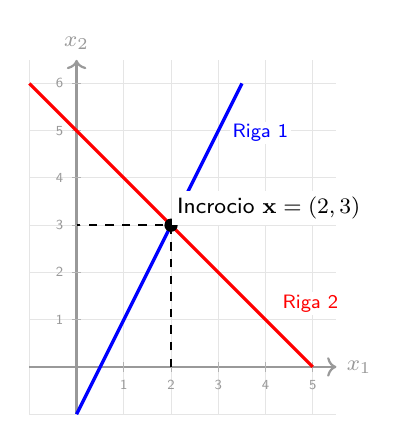
\begin{tikzpicture}[scale=0.6]
                % Griglia standard
                \draw[step=1cm, gray!20, thin] (-1,-1) grid (5.5, 6.5);
                \draw[->, thick, gray!80] (-1,0) -- (5.5,0) node[right, font=\footnotesize] {$x_1$};
                \draw[->, thick, gray!80] (0,-1) -- (0,6.5) node[above, font=\footnotesize] {$x_2$};
                
                % Ticks e numeri
                \foreach \x in {1, 2, 3, 4, 5} \draw[gray!60] (\x, -0.1) -- (\x, 0.1) node[below=3pt, font=\tiny, text=gray!80] {\x};
                \foreach \y in {1, 2, 3, 4, 5, 6} \draw[gray!60] (-0.1, \y) -- (0.1, \y) node[left=3pt, font=\tiny, text=gray!80] {\y};

                % Retta 1 (y = 2x - 1)
                \draw[very thick, blue] (0,-1) -- (3.5,6) node[pos=0.85, right=4pt, font=\scriptsize, fill=white, inner sep=1pt] {Riga 1};
                
                % Retta 2 (y = -x + 5)
                \draw[very thick, red] (-1,6) -- (5,0) node[pos=0.85, above right=4pt, font=\scriptsize, fill=white, inner sep=1pt] {Riga 2};
                
                % Intersezione (La nostra incognita svelata)
                \fill[black] (2,3) circle (4pt);
                \node[above right, font=\footnotesize, fill=white, inner sep=2pt] at (2,3) {Incrocio $\mathbf{x}=(2,3)$};
                \draw[dashed, black, thick] (2,0) -- (2,3) -- (0,3);
            \end{tikzpicture}
        \end{column}
    \end{columns}
\end{frame}


% --- SLIDE 22a: Matrice Identità ---
\begin{frame}{Matrice Identità ($\mathbf{I}$): Il "Punto Fermo"}
    \begin{columns}[T,onlytextwidth]
        \setlength{\columnsep}{0.25cm}
        \begin{column}{0.48\textwidth}
            \scriptsize
            \vspace{0.1cm}
            \begin{itemize}
                \setlength\itemsep{0.5em}
                \item \textbf{Cos'è}: Una matrice quadrata con \textbf{1} sulla diagonale principale e \textbf{0} ovunque altrove.
                
                \item \textbf{L'equivalente del numero 1}:
                Lascia tutto inalterato. Inoltre, \textbf{è commutativa} (un'eccezione preziosa nel mondo delle matrici!):
                \[ \mathbf{A}\mathbf{I} = \mathbf{I}\mathbf{A} = \mathbf{A} \]
                
                \item \textbf{Esempio numerico (Guarda il grafico)}:
                Se applichiamo l'Identità al nostro vettore $\mathbf{v}$, la combinazione lineare ci restituisce esattamente $\mathbf{v}$:
                \[
                \mathbf{I}\mathbf{v} = \begin{bmatrix} \color{orange}1 & \color{purple}0 \\ \color{orange}0 & \color{purple}1 \end{bmatrix} \begin{bmatrix} 2 \\ 3 \end{bmatrix} = \begin{bmatrix} \color{blue}2 \\ \color{blue}3 \end{bmatrix}
                \]
                \vspace{-0.1cm}
                \textit{\tiny Nota tecnica: per i vettori colonna calcoliamo solo $\mathbf{I}\mathbf{v}$. La scrittura $\mathbf{v}\mathbf{I}$ darebbe errore dimensionale!}
                
                \item \textbf{Geometricamente}:
                \begin{itemize}
                    \item L'asse X (\textcolor{orange}{colonna 1}) resta a \textcolor{orange}{(1, 0)}.
                    \item L'asse Y (\textcolor{purple}{colonna 2}) resta a \textcolor{purple}{(0, 1)}.
                \end{itemize}
                Lo spazio \emph{non si deforma} minimamente.
            \end{itemize}
        \end{column}
        
        \begin{column}{0.50\textwidth}
            \centering
            \vspace{0.1cm}
            
            % Matrice I esplicativa con i colori coerenti
            \[
            \mathbf{I} = \begin{bmatrix} \color{orange}1 & \color{purple}0 \\ \color{orange}0 & \color{purple}1 \end{bmatrix} 
            \implies 
            \begin{cases} 
            \mathbf{I}\hat{i} = (\color{orange}1\color{black}, \color{orange}0\color{black}) \\ 
            \mathbf{I}\hat{j} = (\color{purple}0\color{black}, \color{purple}1\color{black}) 
            \end{cases}
            \]
            \vspace{0.1cm}
            
            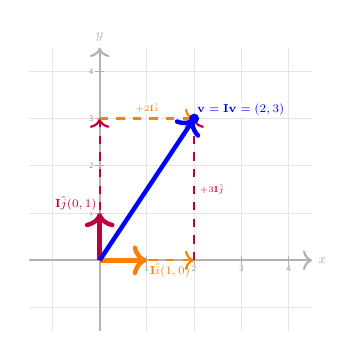
\begin{tikzpicture}[scale=0.6, transform shape]
                % Griglia e Assi (Stessa scala e stile della 21b)
                \draw[step=1cm, gray!20, thin] (-1.5,-1.5) grid (4.5, 4.5);
                \draw[->, thick, gray!60] (-1.5,0) -- (4.5,0) node[right, font=\footnotesize] {$x$};
                \draw[->, thick, gray!60] (0,-1.5) -- (0,4.5) node[above, font=\footnotesize] {$y$};
                
                % Ticks e numeri
                \foreach \x in {1, 2, 3, 4} \draw[gray!60] (\x, -0.1) -- (\x, 0.1) node[below=3pt, font=\tiny, text=gray!80] {\x};
                \foreach \y in {1, 2, 3, 4} \draw[gray!60] (-0.1, \y) -- (0.1, \y) node[left=3pt, font=\tiny, text=gray!80] {\y};

                % Assi identità (I nuovi assi base coincidono con quelli vecchi)
                \draw[->, ultra thick, orange] (0,0) -- (1,0) node[below right, font=\scriptsize, fill=white, inner sep=1pt] {$\mathbf{I}\hat{i}(1,0)$};
                \draw[->, ultra thick, purple] (0,0) -- (0,1) node[above left, font=\scriptsize, fill=white, inner sep=1pt] {$\mathbf{I}\hat{j}(0,1)$};

                % Combinazione Lineare: Costruzione del Parallelogramma "piatto"
                % Lato 1: 2 * Col1 (diventa (2,0))
                \draw[->, thick, orange, dashed] (0,0) -- (2,0);
                % Lato 2: 3 * Col2 (diventa (0,3))
                \draw[->, thick, purple, dashed] (0,0) -- (0,3);

                % Chiusura del parallelogramma (Mostra l'addizione vettoriale esatta, un rettangolo perfetto stavolta)
                \draw[->, thick, purple, dashed] (2,0) -- (2,3) node[midway, right=2pt, font=\tiny, fill=white, inner sep=1pt] {$+3\mathbf{I}\hat{j}$};
                \draw[->, thick, orange, dashed] (0,3) -- (2,3) node[midway, above=2pt, font=\tiny, fill=white, inner sep=1pt] {$+2\mathbf{I}\hat{i}$};

                % Result node (Il vettore v che non si muove)
                \draw[->, ultra thick, blue] (0,0) -- (2,3) node[above right, font=\scriptsize, fill=white, inner sep=1pt] {$\mathbf{v} = \mathbf{I}\mathbf{v} = (2,3)$};
                \fill[blue] (2,3) circle (3pt);

            \end{tikzpicture}
        \end{column}
    \end{columns}
\end{frame}

% --- SLIDE 22b: Determinante ---
\begin{frame}{Il Determinante: Il Fattore di Scala dell'Area}
    \begin{columns}[T] % Allineamento in alto
        
        % --- COLONNA SINISTRA: Concetti ---
        \begin{column}{0.52\textwidth}
            \scriptsize
            \setlength\itemsep{0.2em}
            
            \begin{itemize}
                \item \textbf{Concetto Intuitivo}: 
                Misura quanto area/volume viene espanso o compresso dalla trasformazione.
                
                \item \textbf{Calcolo (2x2)}: 
                Differenza dei prodotti incrociati.
                \[
                    \det(\mathbf{A}) = (\text{a} \cdot \text{d}) - (\text{b} \cdot \text{c})
                \]
                \vspace{-0.45cm}
                Nel nostro esempio:
                \[
                \det\begin{bmatrix} \color{orange}2 & \color{purple}-1 \\ \color{orange}1 & \color{purple}1 \end{bmatrix}
                = (\color{orange}2\color{black}\cdot\color{purple}1\color{black}) - (\color{purple}-1\color{black}\cdot\color{orange}1\color{black})
                = 3
                \]
                
                \vspace{-0.25cm}
                \textit{L'area base (1) viene \textbf{triplicata}: area finale 3.}
                
                \item \textbf{Significato dei Valori}:
                \begin{itemize}
                    \setlength\itemsep{0.05em}
                    \item $\det > 1$: area \textbf{espansa}.
                    \item $\det = 1$: area invariata.
                    \item $0 < \det < 1$: area \textbf{compressa}.
                    \item $\det < 0$: spazio \textbf{ribaltato}.
                \end{itemize}

                \item \textbf{Il Collasso ($\det=0$)}:
                L'area diventa zero: il piano si schiaccia su una linea, trasformazione \textbf{non invertibile}.
            \end{itemize}
        \end{column}
        
        % --- COLONNA DESTRA: Visualizzazioni ---
        \begin{column}{0.48\textwidth}
            \centering
            
            % 1. CALCOLO VISIVO
            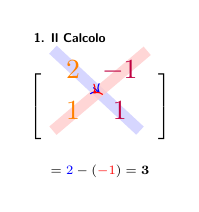
\begin{tikzpicture}[scale=0.66, transform shape]
                \node[anchor=west, font=\scriptsize\bfseries, color=black] at (-1.4, 1.0) {1. Il Calcolo};
                
                % Matrice (Il nostro esempio fisso)
                \matrix [matrix of math nodes, left delimiter={[}, right delimiter={]}, nodes={minimum size=0.5cm}, ampersand replacement=\&] (m) at (0,0) {
                    \color{orange}2 \& \color{purple}-1 \\
                    \color{orange}1 \& \color{purple}1 \\
                };
                
                % Evidenziatori sfondo
                \begin{scope}[on background layer]
                    \draw[line width=4pt, blue!20, opacity=0.8] (m-1-1.north west) -- (m-2-2.south east);
                    \draw[line width=4pt, red!20, opacity=0.8] (m-1-2.north east) -- (m-2-1.south west);
                \end{scope}
                
                % Frecce indicatori
                \draw[->, thin, blue] (m-1-1) -- (m-2-2);
                \draw[->, thin, red] (m-1-2) -- (m-2-1);
                
                \node[below=0.35cm of m, font=\scriptsize] {$= \textcolor{blue}{2} - (\textcolor{red}{-1}) = \mathbf{3}$};
            \end{tikzpicture}
            
            \vspace{0.03cm}
            {\color{gray!40}\hrulefill}
            \vspace{0.03cm}

            % 2. GEOMETRIA (Concepito sulla nostra matrice A)
            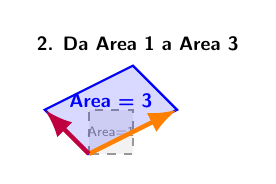
\begin{tikzpicture}[scale=0.56, >=Latex]
                \node[anchor=west, font=\scriptsize\bfseries, color=black] at (-1.4, 2.5) {2. Da Area 1 a Area 3};
            
                \coordinate (O) at (0,0);
                \coordinate (Vi) at (2,1);   % La nostra Col 1 (Arancione)
                \coordinate (Vj) at (-1,1);  % La nostra Col 2 (Viola)
                \coordinate (Sum) at (1,2);  % Vi + Vj

                % Input (Tratteggiato, il quadrato base unitario)
                \draw[thick, dashed, gray!80, fill=gray!10] (0,0) rectangle (1,1);
                \node[font=\tiny, color=gray!90] at (0.5, 0.5) {Area=1};

                % Output (Parallelogramma della nostra matrice)
                \fill[blue, opacity=0.15] (O) -- (Vi) -- (Sum) -- (Vj) -- cycle;
                \draw[thick, blue] (O) -- (Vi) -- (Sum) -- (Vj) -- cycle;
                
                % Vettori Colonna coerenti con i colori
                \draw[->, ultra thick, orange] (O) -- (Vi);
                \draw[->, ultra thick, purple] (O) -- (Vj);
                
                % Label Area
                \node[font=\bfseries\scriptsize, text=blue] at (0.5, 1.2) {Area = 3};
            \end{tikzpicture}

            \vspace{0.03cm}
            {\color{gray!40}\hrulefill}
            \vspace{0.03cm}

            % 3. COLLASSO
            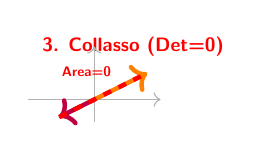
\begin{tikzpicture}[scale=0.56]
                \node[anchor=west, font=\scriptsize\bfseries, color=red] at (-1.4, 1.2) {3. Collasso (Det=0)};
                
                % Assi sfumati
                \draw[->, thin, gray!60] (-1.5,0) -- (1.5,0);
                \draw[->, thin, gray!60] (0,-0.5) -- (0,1.2);
                
                % Linea schiacciata (Vettori colineari)
                \draw[->, ultra thick, orange] (0,0) -- (1.2,0.6);
                \draw[->, ultra thick, purple] (0,0) -- (-0.8,-0.4);
                
                % Area collassata
                \draw[ultra thick, red, dashed] (-0.8,-0.4) -- (1.2,0.6);
                \node[above left, font=\tiny\bfseries, color=red] at (0.6, 0.3) {Area=0};
            \end{tikzpicture}

        \end{column}
    \end{columns}
\end{frame}

% --- SLIDE 22c: Matrice Inversa ---
\begin{frame}{Matrice Inversa ($\mathbf{A}^{-1}$): Il Tasto "Undo"}
    \begin{columns}[T,onlytextwidth]
        \setlength{\columnsep}{0.25cm}
        
        \begin{column}{0.48\textwidth}
            \scriptsize
            \begin{itemize}
                \setlength\itemsep{0.2em}
                \item \textbf{Concetto}: $\mathbf{A}^{-1}$ annulla la deformazione di $\mathbf{A}$ e riporta alla griglia originale.
                
                \item \textbf{Definizione Matematica}:
                Moltiplicare per l'inversa restituisce la matrice identità:
                \[ \mathbf{A}^{-1}\mathbf{A} = \mathbf{A}\mathbf{A}^{-1} = \mathbf{I} \]
                
                \item \textbf{Il nostro Esempio}:
                $\mathbf{A}$ trasforma $\mathbf{v}(2,3)$ in $\mathbf{b}(1,5)$.
                \[ \mathbf{A}\mathbf{v} = \mathbf{b} \implies \mathbf{v} = \mathbf{A}^{-1}\mathbf{b} \]
                L'inversa prende $\mathbf{b}$ nello spazio deformato e recupera le coordinate originali $\mathbf{v}$.
                
                \item \textbf{Requisiti Fondamentali}:
                \begin{itemize}
                    \setlength\itemsep{0.1em}
                    \item $\mathbf{A}$ deve essere \textbf{quadrata} (n° righe = n° colonne).
                    \item $\det(\mathbf{A}) \neq 0$ (Matrice \textbf{Non Singolare}).
                \end{itemize}
                
                \item \textbf{Perché il Det non può essere 0?}
                Se $\det=0$, il piano 2D collassa in 1D: più punti finiscono nello stesso punto, quindi la trasformazione non è invertibile.
            \end{itemize}
        \end{column}
        
        \begin{column}{0.50\textwidth}
            \centering
            \scriptsize
            \vspace{0.04cm}
            
            % DIAGRAMMA DI FLUSSO
            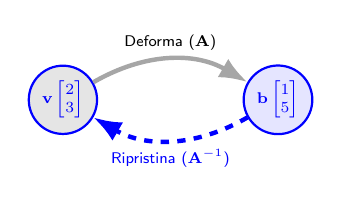
\begin{tikzpicture}[node distance=1.6cm, >=Latex, scale=0.8, transform shape]
                % Nodi
                \node[circle, fill=gray!20, text=blue, font=\scriptsize\bfseries, inner sep=2pt, draw=blue, thick] (v) {$\mathbf{v} \begin{bmatrix} 2 \\ 3 \end{bmatrix}$};
                \node[circle, fill=blue!10, text=blue, font=\scriptsize\bfseries, right=2.3cm of v, inner sep=2pt, draw=blue, thick] (b) {$\mathbf{b} \begin{bmatrix} 1 \\ 5 \end{bmatrix}$};
                
                % Freccia Andata
                \draw[->, ultra thick, gray!70] (v) to[bend left=30] node[midway, above, font=\scriptsize, color=black] {Deforma ($\mathbf{A}$)} (b);
                
                % Freccia Ritorno
                \draw[->, ultra thick, blue, dashed] (b) to[bend left=30] node[midway, below, font=\scriptsize, color=blue] {Ripristina ($\mathbf{A}^{-1}$)} (v);
            \end{tikzpicture}
            
            \vspace{0.06cm}
            {\color{gray!40}\hrulefill}
            \vspace{0.06cm}

            % RAPPRESENTAZIONE VISIVA DEL "RITORNO"
            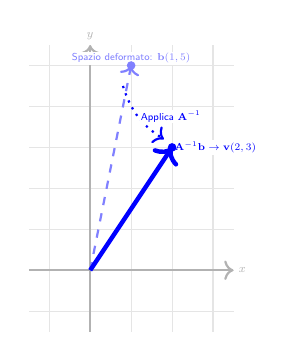
\begin{tikzpicture}[scale=0.52, transform shape]
                % Sfondo: Griglia originale (Quella in cui vogliamo tornare)
                \draw[step=1cm, gray!20, thin] (-1.5,-1.5) grid (3.5, 5.5);
                \draw[->, thick, gray!60] (-1.5,0) -- (3.5,0) node[right, font=\footnotesize] {$x$};
                \draw[->, thick, gray!60] (0,-1.5) -- (0,5.5) node[above, font=\footnotesize] {$y$};

                % L'azione di A-1: prende il vettore b e lo "tira" indietro su v
                
                % Vettore b (Arrivo dalla slide 21b)
                \draw[->, thick, blue!50, dashed] (0,0) -- (1,5) node[above, font=\scriptsize, fill=white, inner sep=1pt] {Spazio deformato: $\mathbf{b}(1,5)$};
                \fill[blue!50] (1,5) circle (3pt);

                % Vettore v (Recuperato)
                \draw[->, ultra thick, blue] (0,0) -- (2,3) node[right, font=\scriptsize, fill=white, inner sep=1pt] {$\mathbf{A}^{-1}\mathbf{b} \to \mathbf{v}(2,3)$};
                \fill[blue] (2,3) circle (3pt);
                
                % Curva di trasformazione (Mostra l'azione Undo)
                \draw[->, thick, blue, dotted, bend right=20] (0.8, 4.5) to node[midway, right=1pt, font=\scriptsize, fill=white, inner sep=0.5pt] {Applica $\mathbf{A}^{-1}$} (1.8, 3.2);

            \end{tikzpicture}
        \end{column}
    \end{columns}
\end{frame}


% --- SLIDE 22c: Solving System ---
\begin{frame}{Applicazione: Risolvere Sistemi Lineari}
    \begin{columns}[T]
        \begin{column}{0.55\textwidth}
            \begin{itemize}
                \setlength\itemsep{0.8em}
                \item \textbf{Perché ci serve?} Per trovare i parametri nascosti di un modello.
                \item \textbf{Mapping nel Machine Learning}:
                \begin{itemize}
                    \item $\color{Dark}\mathbf{A}$: Dati / Features (es. mq, stanze).
                    \item $\color{Secondary}\mathbf{x}$: Pesi / Parametri da imparare.
                    \item $\color{Accent}\mathbf{b}$: Target / Etichette (es. prezzi).
                \end{itemize}
                \item \textbf{Soluzione Analitica}:
                \[ \mathbf{A}\mathbf{x} = \mathbf{b} \implies \mathbf{x} = \mathbf{A}^{-1}\mathbf{b} \]
                \item Trova il vettore $\mathbf{x}$ che mappa i dati $\mathbf{A}$ nel risultato $\mathbf{b}$.
            \end{itemize}
        \end{column}
        \begin{column}{0.45\textwidth}
            \centering
            \vspace{0.5cm}
            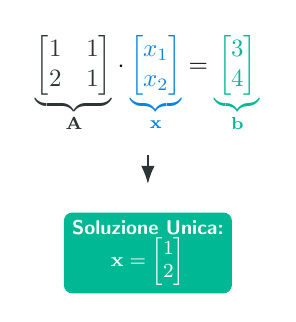
\begin{tikzpicture}[scale=0.9, transform shape]
                % Equations styled
                \node (eq) {
                    $\textcolor{Dark}{\underbrace{\begin{bmatrix} 1 & 1 \\ 2 & 1 \end{bmatrix}}_{\mathbf{A}}}
                     \cdot
                     \textcolor{Secondary}{\underbrace{\begin{bmatrix} x_1 \\ x_2 \end{bmatrix}}_{\mathbf{x}}}
                     =
                     \textcolor{Accent}{\underbrace{\begin{bmatrix} 3 \\ 4 \end{bmatrix}}_{\mathbf{b}}}$
                };
                
                % Arrow down
                \draw[arrow, shorten >=5pt, shorten <=5pt] (eq.south) -- ++(0,-0.8);
                
                % Solution
                \node[accentnode, below=1cm of eq] (sol) {
                    Soluzione Unica:\\
                    $\mathbf{x} = \begin{bmatrix} 1 \\ 2 \end{bmatrix}$
                };
            \end{tikzpicture}
        \end{column}
    \end{columns}
\end{frame}

% --- SLIDE INTRO 1: La "Guerra" delle Lettere ---
\begin{frame}{Dal Liceo al Deep Learning: Cambio di Prospettiva}
    \begin{columns}[T]
        \begin{column}{0.48\textwidth}
            \vspace{0.2cm}
            \small
            \begin{itemize}
                \setlength\itemsep{0.7em}
                \item \textbf{Il Punto di Partenza}: Al liceo impariamo a risolvere \textit{sistemi di equazioni} simultanee.
                
                \item \textbf{La Rivoluzione}: Invece di scrivere decine di equazioni, le "impacchettiamo" in matrici per farle calcolare ai computer.
                
                \item \textbf{L'Ostacolo}: Passando dall'Algebra Lineare classica alle Reti Neurali, le lettere cambiano significato!
            \end{itemize}
            
            \vspace{0.2cm}
            \begin{alertblock}{Attenzione: La "Guerra" delle Lettere}
                \footnotesize
                \begin{itemize}
                    \setlength\itemsep{0.5em}
                    \item \textbf{Data Science ($\mathbf{A}\mathbf{x} = \mathbf{b}$)}: 
                    $\mathbf{A}$ è l'\textit{intero dataset}. Ogni riga è un esempio. Il vettore $\mathbf{x}$ contiene le incognite (i \textbf{Pesi}).
                    
                    \item \textbf{Deep Learning ($\mathbf{y} = \mathbf{W}\mathbf{x}$)}: 
                    Si elabora \textit{un singolo esempio} per volta. Il vettore $\mathbf{x}$ (l'Input) è \textbf{una singola riga di $\mathbf{A}$ messa in verticale}. I pesi diventano $\mathbf{W}$.
                \end{itemize}
            \end{alertblock}
            
        \end{column}
        
        \begin{column}{0.52\textwidth}
            \centering
            
            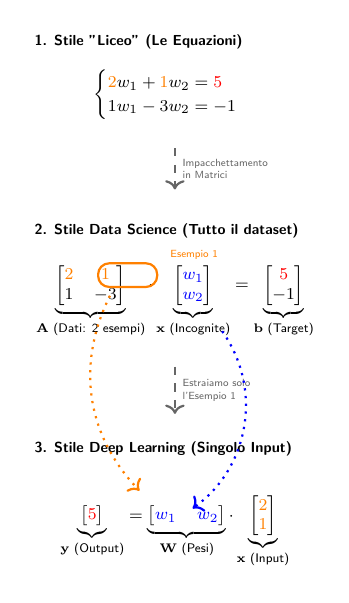
\begin{tikzpicture}[scale=0.75, transform shape]
                
                % 1. Stile Liceo
                \node[anchor=west, font=\scriptsize\bfseries, color=black] at (-2.5, 4.3) {1. Stile "Liceo" (Le Equazioni)};
                
                \node[font=\footnotesize] (liceo) at (0, 3.4) {
                    $\begin{cases} 
                        \color{orange}2\color{black}w_1 + \color{orange}1\color{black}w_2 = \color{red}5 \\ 
                        1w_1 - 3w_2 = -1 
                    \end{cases}$
                };
                
                \draw[->, thick, black!60, dashed] (0, 2.5) -- (0, 1.8) node[midway, right, font=\tiny, align=left] {Impacchettamento\\in Matrici};

                % 2. Stile Data Science
                \node[anchor=west, font=\scriptsize\bfseries, color=black] at (-2.5, 1.1) {2. Stile Data Science (Tutto il dataset)};
                
                \node[font=\footnotesize] (ds) at (0, -0.1) {
                    $\underbrace{\begin{bmatrix} 
                        \color{orange}2 & \color{orange}1 \\ 
                        1 & -3 
                    \end{bmatrix}}_{\mathbf{A} \text{ (Dati: 2 esempi)}}
                    \cdot \underbrace{\begin{bmatrix} \color{blue}w_1 \\ \color{blue}w_2 \end{bmatrix}}_{\mathbf{x} \text{ (Incognite)}}
                    = \underbrace{\begin{bmatrix} \color{red}5 \\ -1 \end{bmatrix}}_{\mathbf{b} \text{ (Target)}}$
                };
                
                % Evidenzia la prima riga di A
                \draw[orange, thick, rounded corners] (-1.3, 0.15) rectangle (-0.3, 0.55);
                \node[orange, font=\tiny, anchor=west] at (-0.2, 0.7) {Esempio 1};

                % Freccia di transizione
                \draw[->, thick, black!60, dashed] (0, -1.2) -- (0, -2.0) node[midway, right, font=\tiny, align=left] {Estraiamo solo\\l'Esempio 1};

                % 3. Stile Deep Learning
                \node[anchor=west, font=\scriptsize\bfseries, color=black] at (-2.5, -2.6) {3. Stile Deep Learning (Singolo Input)};
                
                \node[font=\footnotesize] (dl) at (0, -4.0) {
                    $\underbrace{\begin{bmatrix} \color{red}5 \end{bmatrix}}_{\mathbf{y} \text{ (Output)}}
                    = 
                    \underbrace{\begin{bmatrix} \color{blue}w_1 & \color{blue}w_2 \end{bmatrix}}_{\mathbf{W} \text{ (Pesi)}}
                    \cdot \underbrace{\begin{bmatrix} \color{orange}2 \\ \color{orange}1 \end{bmatrix}}_{\mathbf{x} \text{ (Input)}}$
                };
                
                % Frecce guida curve per mostrare lo spostamento (sottili e non invasive)
                % Riga dei dati -> Vettore colonna Input
                \draw[->, orange, dotted, thick, bend right=35] (-1.1, -0.0) to (-0.6, -3.3);
                
                % Vettore dei Pesi -> Matrice riga W
                \draw[->, blue, dotted, thick, bend left=45] (0.8, -0.6) to (0.3, -3.6);
                
            \end{tikzpicture}
        \end{column}
    \end{columns}
\end{frame}

% --- SLIDE INTRO 2 (Bonus): La Geometria Nascosta ---
\begin{frame}{Geometria a Confronto: Chi definisce lo Spazio?}
    \begin{columns}[T,onlytextwidth]
        \setlength{\columnsep}{0.6cm}
        
        % ==========================================
        % DATA SCIENCE
        % ==========================================
        \begin{column}{0.48\textwidth}
            
            \textbf{\large 1. Data Science ($\mathbf{A}\mathbf{x} = \mathbf{b}$)}
            
            \vspace{0.2cm}
            \footnotesize
            \textbf{La Matrice $\mathbf{A}$ (Dati) = Il Terreno}\\
            Le colonne di $\mathbf{A}$ definiscono gli assi dello spazio. Lo spazio è il \textit{mondo reale} misurato dai nostri dati.
            
            \vspace{0.2cm}
            \textbf{Il Vettore $\mathbf{x}$ (Pesi) = I Passi}\\
            Le nostre incognite $\mathbf{x}$ ci dicono di quanto muoverci lungo gli assi dei dati per raggiungere il bersaglio $\mathbf{b}$.
            
            \vspace{0.2cm}
            \textit{\color{black!70} "Cerchiamo il percorso in un mondo fisso."}
            
            \vspace{0.6cm}
            \centering
            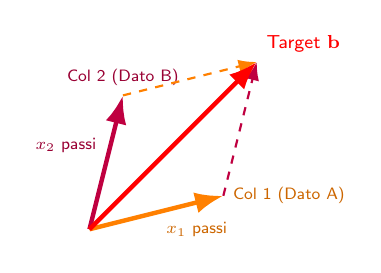
\begin{tikzpicture}[scale=0.85, transform shape, >=Latex]
                % Assi dati (A)
                \draw[->, ultra thick, orange] (0,0) -- (2,0.5) node[right, font=\scriptsize, text=orange!80!black] {Col 1 (Dato A)};
                \draw[->, ultra thick, purple] (0,0) -- (0.5,2) node[above, font=\scriptsize, text=purple!80!black] {Col 2 (Dato B)};
                
                % Linee guida (Parallelogramma)
                \draw[->, thick, orange, dashed] (0.5,2) -- (2.5,2.5);
                \draw[->, thick, purple, dashed] (2,0.5) -- (2.5,2.5);
                
                % Etichette passi
                \node[font=\scriptsize, color=orange!80!black, below right=1pt] at (1, 0.25) {$x_1$ passi};
                \node[font=\scriptsize, color=purple!80!black, above left=1pt] at (0.25, 1) {$x_2$ passi};
                
                % Target b
                \draw[->, ultra thick, red] (0,0) -- (2.5, 2.5) node[above right, font=\footnotesize] {Target $\mathbf{b}$};
            \end{tikzpicture}
            
        \end{column}
        
        % ==========================================
        % DEEP LEARNING
        % ==========================================
        \begin{column}{0.48\textwidth}
            
            \textbf{\large 2. Deep Learning ($\mathbf{y} = \mathbf{W}\mathbf{x}$)}
            
            \vspace{0.2cm}
            \footnotesize
            \textbf{La Matrice $\mathbf{W}$ (Pesi) = Il Terreno}\\
            Le colonne di $\mathbf{W}$ creano i \textit{nuovi assi}. Lo spazio non è quello dei dati, ma uno spazio "inventato" dalla rete.
            
            \vspace{0.2cm}
            \textbf{Il Vettore $\mathbf{x}$ (Input) = I Passi}\\
            L'input ci dice quanto "attivare" ogni asse. I dati sono solo indicazioni per navigare nello spazio della rete.
            
            \vspace{0.2cm}
            \textit{\color{black!70} "Costruiamo noi lo spazio di esplorazione."}
            
            \vspace{0.6cm}
            \centering
            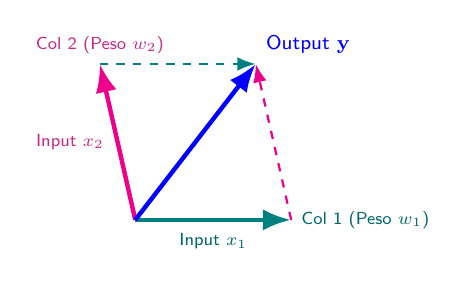
\begin{tikzpicture}[scale=0.9, transform shape, >=Latex]
                % Assi pesi (W)
                \draw[->, ultra thick, teal] (0,0) -- (2.2,0) node[right, font=\scriptsize, text=teal!80!black] {Col 1 (Peso $w_1$)};
                \draw[->, ultra thick, magenta] (0,0) -- (-0.5,2.2) node[above, font=\scriptsize, text=magenta!80!black] {Col 2 (Peso $w_2$)};
                
                % Linee guida (Parallelogramma)
                \draw[->, thick, teal, dashed] (-0.5,2.2) -- (1.7,2.2);
                \draw[->, thick, magenta, dashed] (2.2,0) -- (1.7,2.2);
                
                % Etichette attivazione
                \node[font=\scriptsize, color=teal!80!black, below=2pt] at (1.1, 0) {Input $x_1$};
                \node[font=\scriptsize, color=magenta!80!black, left=2pt] at (-0.25, 1.1) {Input $x_2$};
                
                % Output y
                \draw[->, ultra thick, blue] (0,0) -- (1.7, 2.2) node[above right, font=\footnotesize] {Output $\mathbf{y}$};
            \end{tikzpicture}
            
        \end{column}
    \end{columns}
\end{frame}

% --- SLIDE INTRO 1: Anatomia N vs M ---
\begin{frame}{Anatomia di un Sistema Lineare nel Machine Learning}
    \begin{columns}[T]
        \begin{column}{0.50\textwidth}
            \small
            \vspace{0.2cm}
            \begin{itemize}
                \setlength\itemsep{1.2em}
                \item Il sistema $\mathbf{A}\mathbf{x} = \mathbf{b}$ è la mappa del nostro dataset.
                
                \item \textbf{$\mathbf{A}$ (Matrice Dati)}:
                \begin{itemize}
                    \item \textbf{$N$ (Righe)}: Il numero di \textit{Esempi} o osservazioni (es. 100 case vendute).
                    \item \textbf{$M$ (Colonne)}: Il numero di \textit{Features} o variabili (es. Mq, Stanze, Zona).
                \end{itemize}
                
                \item \textbf{$\mathbf{x}$ (Pesi)}:
                Sono le $M$ incognite che vogliamo scoprire. Quanto "conta" ogni feature?
                
                \item \textbf{$\mathbf{b}$ (Target)}:
                Sono gli $N$ risultati reali osservati (es. i prezzi delle case).
            \end{itemize}
        \end{column}
        
        \begin{column}{0.50\textwidth}
            \centering
            % VISUALIZZAZIONE MATRICE N x M
            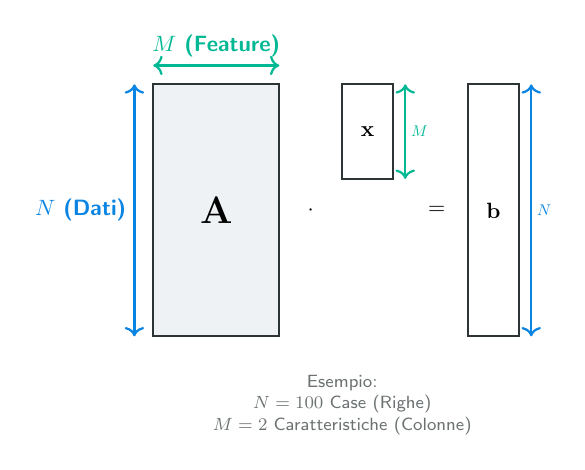
\begin{tikzpicture}[scale=0.8, transform shape]
                
                % Matrice A (Rettangolare Alta - N > M)
                \fill[Light!50] (0,0) rectangle (2,4);
                \draw[thick, Dark] (0,0) rectangle (2,4);
                \node at (1, 2) {\LARGE $\mathbf{A}$};
                
                % Quote N e M
                \draw[<->, Secondary, thick] (-0.3, 0) -- (-0.3, 4) node[midway, left] {\textbf{$N$ (Dati)}};
                \draw[<->, Accent, thick] (0, 4.3) -- (2, 4.3) node[midway, above] {\textbf{$M$ (Feature)}};
                
                % Vettore x
                \node at (2.5, 2) {$\cdot$};
                \draw[thick, Dark] (3, 2.5) rectangle (3.8, 4); 
                \node at (3.4, 3.25) {$\mathbf{x}$};
                \draw[<->, Accent, thick] (4.0, 2.5) -- (4.0, 4) node[midway, right, scale=0.7] {$M$};

                % Uguale b
                \node at (4.5, 2) {$=$};
                \draw[thick, Dark] (5, 0) rectangle (5.8, 4);
                \node at (5.4, 2) {$\mathbf{b}$};
                \draw[<->, Secondary, thick] (6.0, 0) -- (6.0, 4) node[midway, right, scale=0.7] {$N$};
                
                % Esempio testuale sotto
                \node[below=0.5cm, align=center, font=\footnotesize, color=Dark!70] at (3,0) {
                    Esempio:\\
                    $N=100$ Case (Righe)\\
                    $M=2$ Caratteristiche (Colonne)
                };
            \end{tikzpicture}
        \end{column}
    \end{columns}
\end{frame}

% --- SLIDE GEOMETRIA 1: I Dati nello Spazio (2D) ---
\begin{frame}{Dai Numeri allo Spazio: Il Caso Semplice (2D)}
\begin{columns}[T]
    \begin{column}{0.55\textwidth}
        \small % Rimpicciolisce leggermente il testo per sicurezza
        \begin{itemize}
            \setlength\itemsep{0.8em} % Spaziatura ridotta
            \item \textbf{Partiamo da un caso base}:
            \begin{itemize}
                \item Immaginiamo \textbf{1 Feature} ($M=1$, es. $m^2$) e \textbf{1 Target} (es. il Prezzo).
            \end{itemize}
            \item Ogni riga del dataset (un singolo esempio) diventa un \textbf{punto esatto} su un piano.
            \item \textbf{Cosa sono le coordinate?}
            \begin{itemize}
                \item La matrice $\mathbf{A}$ ci dà la posizione sull'asse orizzontale.
                \item Il vettore $\mathbf{b}$ ci dà l'altezza sull'asse verticale.
            \end{itemize}
        \end{itemize}
    \end{column}
    
    \begin{column}{0.45\textwidth}
        \centering
        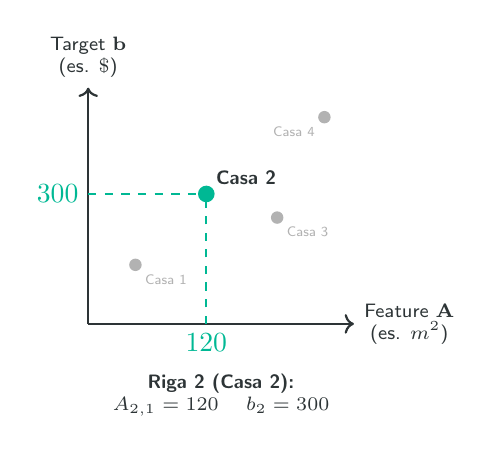
\begin{tikzpicture}[scale=0.75] % Scalato per non sbordare
            
            % Assi
            \draw[->, thick, Dark] (0,0) -- (4.5,0) node[right, align=center, font=\scriptsize] {Feature $\mathbf{A}$\\(es. $m^2$)};
            \draw[->, thick, Dark] (0,0) -- (0,4.0) node[above, align=center, font=\scriptsize] {Target $\mathbf{b}$\\(es. $\$$)};
            
            % Punti dati "anonimi"
            \fill[gray!60] (0.8, 1.0) circle (3pt) node[below right, font=\tiny] {Casa 1};
            \fill[gray!60] (3.2, 1.8) circle (3pt) node[below right, font=\tiny] {Casa 3};
            \fill[gray!60] (4.0, 3.5) circle (3pt) node[below left, font=\tiny] {Casa 4};
            
            % Punto Evidenziato (Casa 2)
            \fill[Accent] (2.0, 2.2) circle (4pt) node[above right, text=Dark, font=\bfseries\scriptsize] {Casa 2};
            
            % Linee guida
            \draw[dashed, Accent, thick] (2.0,0) -- (2.0,2.2);
            \draw[dashed, Accent, thick] (0,2.2) -- (2.0,2.2);
            
            % Etichette sugli assi
            \node[below, font=\small, text=Accent, font=\bfseries] at (2.0,0) {$120$};
            \node[left, font=\small, text=Accent, font=\bfseries] at (0,2.2) {$300$};
            
            % Didascalia spostata in basso per non sovrapporsi all'asse Y
            \node[align=center, font=\scriptsize, color=Dark] at (2.25, -1.2) {
                \textbf{Riga 2 (Casa 2):}\\
                $A_{2,1} = 120$ \quad $b_2 = 300$
            };
        \end{tikzpicture}
    \end{column}
\end{columns}
\end{frame}

% --- SLIDE GEOMETRIA 2: Il Mondo Reale (Iper-spazio) ---
\begin{frame}{Dai Numeri allo Spazio: Il Mondo Reale}
\begin{columns}[T]
    \begin{column}{0.55\textwidth}
        \small
        \begin{itemize}
            \setlength\itemsep{0.7em} % Spaziatura ridotta per far stare tutto
            \item \textbf{Aggiungiamo complessità}:
            \begin{itemize}
                \item E se avessimo \textbf{10 feature} ($M=10$, es. $m^2$, stanze, bagni...)?
            \end{itemize}
            \item Geometricamente, ogni nuova feature aggiunge un \textbf{nuovo asse} al nostro grafico.
            \item Ogni casa ora vive in uno \textbf{spazio a 11 dimensioni} (10 assi per $\mathbf{A}$, 1 per $\mathbf{b}$).
            \item \textbf{La magia dell'Algebra Lineare}: 
            Non possiamo disegnare 11 dimensioni, ma \emph{le equazioni non cambiano}! Il computer calcola l'intersezione allo stesso modo, in un "iper-spazio".
        \end{itemize}
    \end{column}
    
    \begin{column}{0.45\textwidth}
        \centering
        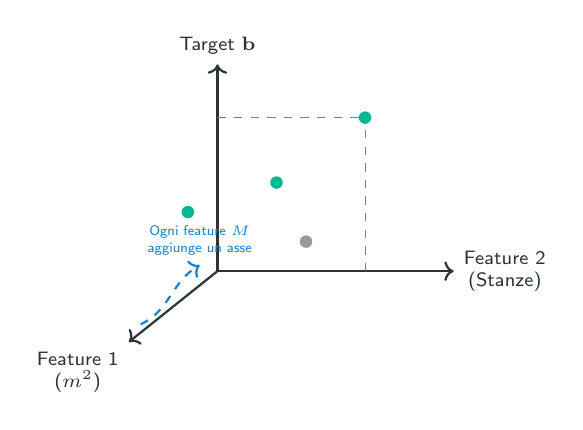
\begin{tikzpicture}[scale=0.75] % Scalato per sicurezza
            
            % Assi 3D finti
            \draw[->, thick, Dark] (0,0) -- (-1.5,-1.2) node[below left, align=center, font=\scriptsize] {Feature 1\\($m^2$)};
            \draw[->, thick, Dark] (0,0) -- (4,0) node[right, align=center, font=\scriptsize] {Feature 2\\(Stanze)};
            \draw[->, thick, Dark] (0,0) -- (0,3.5) node[above, align=center, font=\scriptsize] {Target $\mathbf{b}$};
            
            % Punti sospesi nel 3D
            \fill[Accent] (1, 1.5) circle (3pt);
            \fill[Accent] (2.5, 2.6) circle (3pt);
            \fill[Accent] (-0.5, 1.0) circle (3pt);
            \fill[gray!80] (1.5, 0.5) circle (3pt);
            
            % Linee guida per dare profondità (proiezione finta)
            \draw[dashed, gray] (2.5,0) -- (2.5, 2.6);
            \draw[dashed, gray] (0,2.6) -- (2.5, 2.6);
            
            % Freccia vicino all'asse Feature 1, parte dall'asse
            \draw[->, thick, Secondary, dashed] (-1.3, -0.9) to[out=25, in=210] (-0.3, 0.1)
            node[above, align=center, font=\tiny, text=Secondary] {Ogni feature $M$\\aggiunge un asse};
            
        \end{tikzpicture}
    \end{column}
\end{columns}
\end{frame}

% --- SLIDE GEOMETRIA 2: Cosa fa il sistema lineare ---
\begin{frame}{Il Significato Grafico: Cercare il Modello Perfetto}
\begin{columns}[T]
    \begin{column}{0.5\textwidth}
        \vspace{0.2cm}
        \begin{itemize}
            \setlength\itemsep{1em}
            \item Risolvere il sistema $\mathbf{A}\mathbf{x} = \mathbf{b}$ significa cercare le "regole" (i pesi $\mathbf{x}$).
            \item \textbf{Graficamente}, i pesi $\mathbf{x}$ definiscono una \textbf{retta} (o un iperpiano se $M>1$).
            \item Risolvere il sistema in modo \emph{esatto} significa trovare una retta che \textbf{trafigge perfettamente tutti i punti} del nostro grafico contemporaneamente.
            \item La pendenza e l'inclinazione di questa retta sono proprio i valori del nostro vettore incognito $\mathbf{x}$.
        \end{itemize}
    \end{column}
    
    \begin{column}{0.5\textwidth}
        \centering
        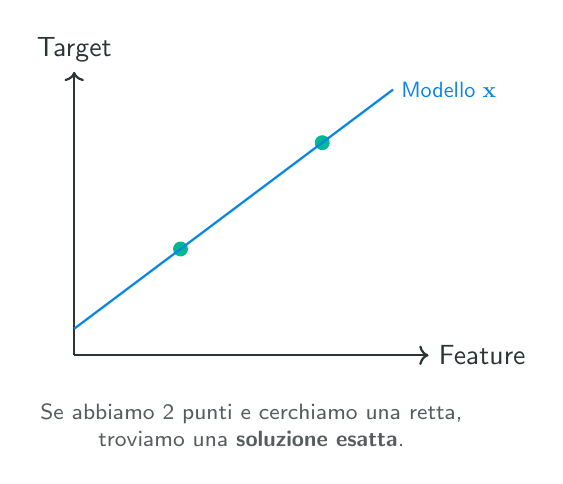
\begin{tikzpicture}[scale=0.9]
            % Assi
            \draw[->, thick, Dark] (0,0) -- (5,0) node[right] {Feature};
            \draw[->, thick, Dark] (0,0) -- (0,4) node[above] {Target};
            
            % Punti (N=2, allineati perfettamente)
            \fill[Accent] (1.5, 1.5) circle (3pt);
            \fill[Accent] (3.5, 3.0) circle (3pt);
            
            % La Retta Perfetta
            \draw[thick, Secondary] (0, 0.375) -- (4.5, 3.75) node[right, scale=0.8] {Modello $\mathbf{x}$};
            
            \node[below=0.5cm, align=center, font=\footnotesize, color=Dark!80] at (2.5,0) {
                Se abbiamo 2 punti e cerchiamo una retta,\\
                troviamo una \textbf{soluzione esatta}.
            };
        \end{tikzpicture}
    \end{column}
\end{columns}
\end{frame}

% --- SLIDE 1: Il Significato Geometrico ---
\begin{frame}{Il Significato Geometrico del Modello}
    \begin{columns}[T]
        \begin{column}{0.45\textwidth}
            \vspace{0.2cm}
            \small
            \begin{itemize}
                \setlength\itemsep{1.2em}
                \item Quando abbiamo \textbf{1 Feature}, il sistema $\mathbf{A}\mathbf{x}=\mathbf{b}$ descrive una \textbf{relazione diretta} tra input e output.
                
                \item \textbf{I protagonisti}:
                \begin{itemize}
                    \item $\mathbf{A}$ (Feature): es. i metri quadri.
                    \item $\mathbf{b}$ (Target): es. il prezzo della casa.
                    \item $\mathbf{x}$ (Peso): \emph{Quanto costa un singolo metro quadro?}
                \end{itemize}
                
                \item \textbf{Cosa stiamo facendo?}
                Stiamo cercando una retta che attraversi i nostri dati nel miglior modo possibile, permettendoci di fare previsioni per il futuro.
            \end{itemize}
        \end{column}
        
        \begin{column}{0.55\textwidth}
            \centering
            % VISUALIZZAZIONE GEOMETRICA
            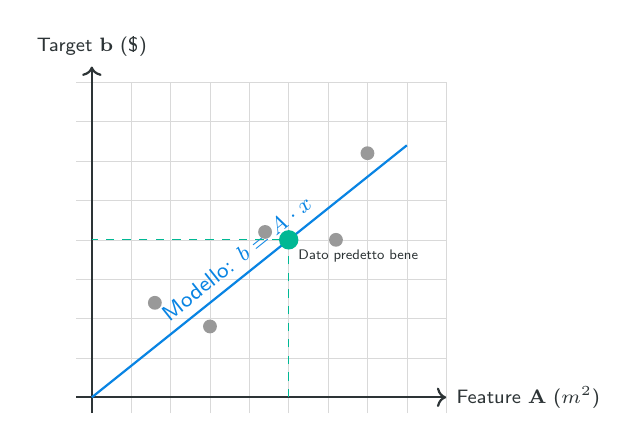
\begin{tikzpicture}[scale=1.0, transform shape]
                % Griglia e Assi
                \draw[help lines, color=gray!30, step=0.5] (-0.2,-0.2) grid (4.5,4.0);
                \draw[->, thick, Dark] (-0.2,0) -- (4.5,0) node[right, font=\scriptsize] {Feature $\mathbf{A}$ ($m^2$)};
                \draw[->, thick, Dark] (0,-0.2) -- (0,4.2) node[above, font=\scriptsize] {Target $\mathbf{b}$ (\$)};
                
                % Retta modello: b = A * x
                \draw[thick, Secondary] (0,0) -- (4.0, 3.2) node[above left, font=\footnotesize, sloped, near end, text=Secondary] {Modello: $b = A \cdot x$};
                
                % Punti dati reali (rumorosi)
                \fill[gray!80] (0.8, 1.2) circle (2.5pt);
                \fill[gray!80] (1.5, 0.9) circle (2.5pt);
                \fill[gray!80] (2.2, 2.1) circle (2.5pt);
                \fill[gray!80] (3.1, 2.0) circle (2.5pt);
                \fill[gray!80] (3.5, 3.1) circle (2.5pt);
                
                % Evidenziare una previsione perfetta
                \fill[Accent] (2.5, 2.0) circle (3.5pt) node[below right, font=\tiny, text=Dark] {Dato predetto bene};
                \draw[dashed, Accent] (2.5,0) -- (2.5,2.0) -- (0,2.0);
            \end{tikzpicture}
        \end{column}
    \end{columns}
\end{frame}

% --- SLIDE 2: Come si costruisce la retta ---
\begin{frame}{Esempio Pratico: Dai Dati alla Retta}
    \begin{columns}[T,onlytextwidth]
        \setlength{\columnsep}{0.2cm}
        
        \begin{column}{0.54\textwidth} % Colonna testo leggermente allargata
            \vspace{0.1cm}
            \small
            \begin{itemize}
                \setlength\itemsep{0.6em} % Spazio tra i bullet ridotto
                
                \item \textbf{1. I Dati Reali (Il Dataset)}\\
                Abbiamo $N=3$ case. $\mathbf{A}$ ha 1 colonna (mq), $\mathbf{b}$ è il prezzo reale:
                \vspace{-0.15cm} % Risparmio spazio verticale
                \[
                \mathbf{A} = \begin{bmatrix} 0.5 \\ 1.2 \\ 2.1 \end{bmatrix} \quad 
                \mathbf{b} = \begin{bmatrix} 1.1 \\ 2.6 \\ 3.9 \end{bmatrix}
                \]
                \vspace{-0.15cm} % Risparmio spazio verticale
                
                \item \textbf{2. Il Modello Matematico}\\
                L'algoritmo trova il peso ottimale: \textbf{$\mathbf{x} = 2$}.\\
                L'equazione per le \textit{previsioni} diventa: \textbf{$\mathbf{b}_{pred} = \mathbf{A} \cdot 2$}
                
                \item \textbf{3. Dal Calcolo al Grafico}\\
                Per disegnare la retta modello ci bastano due punti strategici sull'asse $\mathbf{A}$:
                \begin{itemize}
                    \item Se $\mathbf{A} = 0 \implies \mathbf{b}_{pred} = 0 \cdot 2 = \mathbf{0}$
                    \item Se $\mathbf{A} = 2 \implies \mathbf{b}_{pred} = 2 \cdot 2 = \mathbf{4}$
                \end{itemize}
                
                \vspace{0.1cm}
                \textit{\footnotesize Unendo i punti arancioni (0,0) e (2,4) otteniamo la retta!}
            \end{itemize}
        \end{column}
        
        \begin{column}{0.46\textwidth} % Colonna grafico
            \centering
            \vspace{0.2cm}
            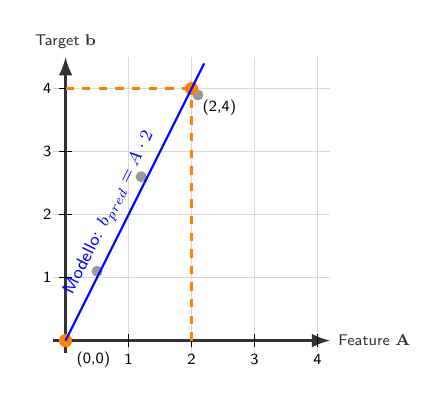
\begin{tikzpicture}[scale=0.8, transform shape, >=Latex] % Scala ridotta a 0.8 per non sbordare
                % Griglia e Assi (Stile continuo con Slide 1)
                \draw[help lines, color=gray!30, step=1.0] (-0.2,-0.2) grid (4.2,4.5);
                \draw[->, thick, black!80] (-0.2,0) -- (4.2,0) node[right, font=\scriptsize] {Feature $\mathbf{A}$};
                \draw[->, thick, black!80] (0,-0.2) -- (0,4.5) node[above, font=\scriptsize] {Target $\mathbf{b}$};
                
                % Ticks
                \foreach \x in {1,2,3,4} \draw (\x,0.1) -- (\x,-0.1) node[below, font=\scriptsize] {\x};
                \foreach \y in {1,2,3,4} \draw (0.1,\y) -- (-0.1,\y) node[left, font=\scriptsize] {\y};
                
                % Punti del dataset A e b reali (Grigi)
                \fill[gray!80] (0.5, 1.1) circle (2.5pt);
                \fill[gray!80] (1.2, 2.6) circle (2.5pt);
                \fill[gray!80] (2.1, 3.9) circle (2.5pt);
                
                % Punti calcolati per tracciare la retta (Arancioni)
                \fill[orange] (0,0) circle (3pt) node[below right=2pt, font=\scriptsize, text=black] {(0,0)};
                \fill[orange] (2,4) circle (3pt) node[below right=2pt, font=\scriptsize, text=black] {(2,4)};
                
                % Linee di costruzione Punto 2
                \draw[dashed, orange, thick] (2,0) -- (2,4);
                \draw[dashed, orange, thick] (0,4) -- (2,4);
                
                % Retta del Modello
                \draw[thick, blue] (0,0) -- (2.2, 4.4) node[above left, font=\footnotesize, sloped, near end, text=blue] {Modello: $b_{pred} = A \cdot 2$};
                
            \end{tikzpicture}
        \end{column}
    \end{columns}
\end{frame}

% --- SLIDE 3: Il Significato della Pendenza ---
\begin{frame}{Analisi del Modello: La Pendenza ($\mathbf{x}$)}
    \begin{columns}[T]
        \begin{column}{0.50\textwidth}
            \vspace{0.2cm}
            \footnotesize
            \begin{itemize}
                \setlength\itemsep{0.6em}
                \item Il valore $\mathbf{x}$ (nel nostro caso $2$) rappresenta la \textbf{pendenza} della retta.
                
                \item \textbf{Significato pratico}:
                Ci dice di quanto sale il target $\mathbf{b}$ se facciamo un "passo" in avanti unitario sulla feature $\mathbf{A}$.
                
                \item \textbf{E l'intercetta (Bias)?}
                Noterai che questa retta parte esattamente da zero $(0,0)$. Nel Machine Learning reale, quasi sempre si aggiunge un parametro fisso (il Bias) per permettere alla retta di partire da un'altezza diversa.
            \end{itemize}
        \end{column}
        
        \begin{column}{0.50\textwidth}
            \centering
            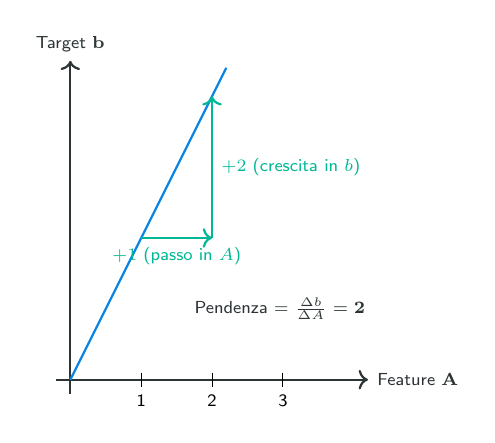
\begin{tikzpicture}[scale=0.9, transform shape]
                % Assi
                \draw[->, thick, Dark] (-0.2,0) -- (4.2,0) node[right, font=\scriptsize] {Feature $\mathbf{A}$};
                \draw[->, thick, Dark] (0,-0.2) -- (0,4.5) node[above, font=\scriptsize] {Target $\mathbf{b}$};
                
                % Ticks
                \foreach \x in {1,2,3} \draw (\x,0.1) -- (\x,-0.1) node[below, font=\scriptsize] {\x};
                
                % Retta
                \draw[thick, Secondary] (0,0) -- (2.2, 4.4);
                
                % Triangolo della pendenza (Rise over Run)
                \draw[thick, Accent, ->] (1,2) -- (2,2) node[midway, below, font=\scriptsize] {$+1$ (passo in $A$)};
                \draw[thick, Accent, ->] (2,2) -- (2,4) node[midway, right, font=\scriptsize] {$+2$ (crescita in $b$)};
                
                \node[align=left, font=\scriptsize, color=Dark] at (3.0, 1.0) {
                    Pendenza = $\frac{\Delta b}{\Delta A} = \mathbf{2}$
                };
            \end{tikzpicture}
        \end{column}
    \end{columns}
\end{frame}

% --- SLIDE 3: Da Retta a Piano ---
\begin{frame}{Aggiungere una Feature: Dalla Retta al Piano}
    \begin{columns}[T,onlytextwidth]
        \setlength{\columnsep}{0.2cm}
        
        \begin{column}{0.54\textwidth}
            \vspace{0.1cm}
            \small
            \begin{itemize}
                \setlength\itemsep{0.6em}
                \item \textbf{1. Due Dimensioni (Es. Mq + Stanze)}\\
                La matrice $\mathbf{A}$ ora ha 2 colonne. Il vettore dei pesi deve avere 2 incognite: $\mathbf{x} = \begin{bmatrix} x_1 \\ x_2 \end{bmatrix}$.
                
                \item \textbf{2. Il Modello Diventa 3D}\\
                L'equazione somma le due feature pesate:\\
                $\mathbf{b}_{pred} = \mathbf{A}_1 \cdot x_1 + \mathbf{A}_2 \cdot x_2$
                
                \item \textbf{3. Costruire il Piano (Esempio)}\\
                L'algoritmo trova $\mathbf{x} = \begin{bmatrix} 2 \\ 1 \end{bmatrix}$ (2k/mq, 1k/stanza).
                Per tracciare un \textbf{piano} ci servono \textbf{3 punti}:
                \begin{enumerate}
                    \item Casa: 0mq, 0st $\implies b = 0(2) \!+\! 0(1) = \mathbf{0}$
                    \item Casa: 2mq, 0st $\implies b = 2(2) \!+\! 0(1) = \mathbf{4}$
                    \item Casa: 0mq, 2st $\implies b = 0(2) \!+\! 2(1) = \mathbf{2}$
                \end{enumerate}
                
                \vspace{0.1cm}
                \textit{\footnotesize Unendo questi 3 punti arancioni, si tende il "lenzuolo" (il piano blu) che approssima i dati reali 3D!}
            \end{itemize}
        \end{column}
        
        \begin{column}{0.46\textwidth}
            \centering
            \vspace{0.1cm}
            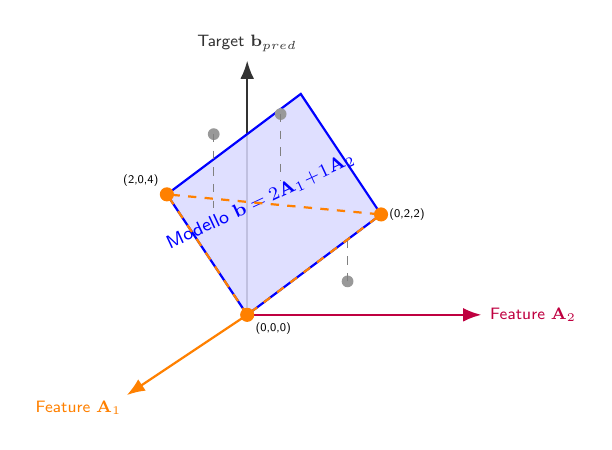
\begin{tikzpicture}[scale=0.85, transform shape, >=Latex]
                % Assi Pseudo-3D
                \coordinate (O) at (0,0);
                \coordinate (X1) at (-1.8, -1.2); % Asse A1 (mq) - Arancione
                \coordinate (X2) at (3.5, 0);     % Asse A2 (stanze) - Viola
                \coordinate (Y) at (0, 3.8);      % Asse b (prezzo) - Nero
                
                \draw[->, thick, orange] (O) -- (X1) node[below left=-2pt, font=\scriptsize] {Feature $\mathbf{A}_1$};
                \draw[->, thick, purple] (O) -- (X2) node[right, font=\scriptsize] {Feature $\mathbf{A}_2$};
                \draw[->, thick, black!80] (O) -- (Y) node[above, font=\scriptsize] {Target $\mathbf{b}_{pred}$};
                
                % 3 Punti Calcolati per generare il piano
                \coordinate (P1) at (0,0);                   % (0,0,0)
                \coordinate (P2) at (-1.2, 1.8);             % Su A1, sollevato di 4
                \coordinate (P3) at (2.0, 1.5);              % Su A2, sollevato di 2
                \coordinate (P4) at (0.8, 3.3);              % Chiusura parallelogramma P2+P3

                % Dati Reali (Grigi) "dietro" e "sotto" il piano
                \fill[gray!80] (1.5, 0.5) circle (2.5pt); % Sotto il piano
                \draw[dashed, gray] (1.5, 0.5) -- (1.5, 1.2); % Errore verso il piano

                % Piano (modello) - con opacità per far vedere la tridimensionalità
                \fill[blue!15, opacity=0.85] (P1) -- (P2) -- (P4) -- (P3) -- cycle;
                \draw[thick, blue] (P1) -- (P2) -- (P4) -- (P3) -- cycle;
                \node[font=\footnotesize, text=blue, rotate=25] at (0.2, 1.7) {Modello $\mathbf{b} = 2\mathbf{A}_1 \!+\! 1\mathbf{A}_2$};
                
                % Linee guida tra i 3 punti strategici
                \draw[dashed, orange, thick] (P1) -- (P2) -- (P3) -- cycle;
                
                % Disegna i 3 punti base (Arancioni)
                \fill[orange] (P1) circle (3pt) node[below right, font=\tiny, text=black] {(0,0,0)};
                \fill[orange] (P2) circle (3pt) node[above left, font=\tiny, text=black] {(2,0,4)};
                \fill[orange] (P3) circle (3pt) node[right, font=\tiny, text=black] {(0,2,2)};
                
                % Dati Reali (Grigi) "davanti" e "sopra" il piano
                \fill[gray!80] (-0.5, 2.7) circle (2.5pt); % Sopra il piano
                \draw[dashed, gray] (-0.5, 2.7) -- (-0.5, 1.6); % Errore verso il piano
                
                \fill[gray!80] (0.5, 3.0) circle (2.5pt); % Sopra il piano
                \draw[dashed, gray] (0.5, 3.0) -- (0.5, 2.0); % Errore verso il piano

            \end{tikzpicture}
        \end{column}
    \end{columns}
\end{frame}


% --- SLIDE 5: Aggiungere Dati (Sistemi Sovradeterminati) ---
\begin{frame}{Aggiungere Dati: Quando l'Algebra "si Rompe"}
    \begin{columns}[T,onlytextwidth]
        \setlength{\columnsep}{0.15cm}
        
        \begin{column}{0.53\textwidth}
            \vspace{-0.05cm}
            \footnotesize
            \begin{itemize}
                \setlength\itemsep{0.35em}
                \item \textbf{Cosa significa "Aggiungere una Retta"?}\\
                Aggiungiamo una \textbf{riga} al sistema $\mathbf{A}\mathbf{x}=\mathbf{b}$. Nella realtà, significa che abbiamo raccolto un \textbf{nuovo dato} (es. una terza casa) per trovare i pesi $x_1$ e $x_2$.
                
                \item \textbf{La Visione per Righe}\\
                Ogni riga-equazione (es. $2x_1 + 1x_2 = 5$) traccia una \textbf{retta} di vincolo. La soluzione perfetta è l'incrocio esatto.
                
                \item \textbf{Il problema dei dati multipli}\\
                Cercare 2 incognite avendo 3 (o più) equazioni crea un sistema \textit{sovradeterminato}.
                
                \vspace{0.05cm}
                \footnotesize
                \begin{itemize}
                    \setlength\itemsep{0.18em}
                    \item \textbf{1 Soluzione (Teoria)}: Incrocio perfetto (rarissimo con dati reali).
                    \item \textbf{0 Soluzioni (Realtà)}: Nessun punto comune. \textbf{Qui nasce il ML}: cerca il punto "centrale" che minimizza l'errore per tutti!
                    \item \textbf{$\infty$ Soluzioni}: Dati perfettamente duplicati.
                \end{itemize}
            \end{itemize}
        \end{column}
        
        \begin{column}{0.47\textwidth}
            \centering
            \vspace{-0.05cm}
            \begin{tikzpicture}[scale=0.66, transform shape, >=Latex]
                
                % Caso 1: Una soluzione (Incrocio perfetto)
                \begin{scope}[shift={(0,4.5)}]
                    \node[anchor=west, font=\scriptsize\bfseries] at (-0.5, 2.2) {1. Incrocio Perfetto (Ideale)};
                    \draw[->, thick, gray!80] (-0.5,0) -- (3.2,0) node[right, font=\scriptsize] {$x_1$};
                    \draw[->, thick, gray!80] (0,-0.2) -- (0,1.8) node[above, font=\scriptsize] {$x_2$};
                    
                    \draw[thick, blue] (0.2, 1.6) -- (2.8, 0.2);  
                    \draw[thick, red] (0.2, 0.2) -- (2.8, 1.6);   
                    \draw[thick, orange] (1.5, 1.8) -- (1.5, 0.0); 
                    
                    \fill[black] (1.5, 0.9) circle (2.5pt); 
                \end{scope}

                % Caso 2: Zero soluzioni (Il triangolo ben distanziato)
                \begin{scope}[shift={(0,1.6)}]
                    \node[anchor=west, font=\scriptsize\bfseries] at (-0.5, 2.2) {2. Zero Soluzioni (Realtà dei Dati)};
                    \draw[->, thick, gray!80] (-0.5,0) -- (3.2,0) node[right, font=\scriptsize] {$x_1$};
                    \draw[->, thick, gray!80] (0,-0.2) -- (0,1.8) node[above, font=\scriptsize] {$x_2$};
                    
                    % Definisco i 3 vertici del triangolo di errore
                    \coordinate (V1) at (0.8, 1.5);
                    \coordinate (V2) at (1.5, 0.5);
                    \coordinate (V3) at (2.4, 1.3);
                    
                    % coloro il triangolo
                    \fill[gray!30, opacity=0.9] (V1) -- (V2) -- (V3) -- cycle;
                    
                    % Rette accorciate: restano nel riquadro del grafico
                    \draw[thick, blue] (0.35, 1.85) -- (1.85, -0.15);
                    \draw[thick, red] (0.95, 0.05) -- (2.65, 1.65);
                    \draw[thick, orange] (0.20, 1.55) -- (2.75, 1.15);
                    
                    % Il punto "Best Fit" (ML) nel baricentro
                    \fill[green!60!black] (1.56, 1.1) circle (2.5pt);
                    \node[font=\scriptsize, text=green!60!black, below=2pt] at (1.56, 1.1) {Best Fit (ML)};
                \end{scope}

                % Caso 3: Infinite soluzioni (Sovrapposizione e ben distanziato)
                \begin{scope}[shift={(0,-1.2)}]
                    \node[anchor=west, font=\scriptsize\bfseries] at (-0.5, 2.2) {3. Infinite Soluzioni ($\infty$)};
                    \draw[->, thick, gray!80] (-0.5,0) -- (3.2,0) node[right, font=\scriptsize] {$x_1$};
                    \draw[->, thick, gray!80] (0,-0.2) -- (0,1.8) node[above, font=\scriptsize] {$x_2$};
                    
                    % Rette sovrapposte
                    \draw[line width=3pt, blue!20] (0.2, 0.4) -- (2.8, 1.4);
                    \draw[thick, dashed, red] (0.2, 0.4) -- (2.8, 1.4);
                    \draw[thick, dotted, orange] (0.2, 0.4) -- (2.8, 1.4);
                    
                    \node[font=\scriptsize, text=black, above left=1pt] at (2.8, 1.4) {Dati identici/multipli};
                \end{scope}
                
            \end{tikzpicture}
        \end{column}
    \end{columns}
\end{frame}

% --- SLIDE 1: Isolare i Pesi (Dall'Algebra al DL) ---
\begin{frame}{Come Isoliamo i Pesi? (Teoria vs Pratica)}
    \begin{columns}[T,onlytextwidth]
        \setlength{\columnsep}{0.3cm}
        
        \begin{column}{0.56\textwidth}
            \vspace{0.1cm}
            \footnotesize
            Fino ad ora abbiamo visto il sistema. Ma il nostro obiettivo è trovare i pesi! Come li isoliamo?
            
            \vspace{0.2cm}
            \textbf{1. Algebra Classica (Sistemi Quadrati)}\\
            La formula è $\mathbf{A}\mathbf{x} = \mathbf{b}$. Se $\mathbf{A}$ è quadrata, passiamo $\mathbf{A}$ dall'altra parte usando l'inversa:
            \[ \mathbf{x} = \mathbf{A}^{-1}\mathbf{b} \]
            
            \vspace{0.1cm}
            \textbf{2. Machine Learning (Minimi Quadrati)}\\
            Il dataset $\mathbf{A}$ è rettangolare. \textbf{Le matrici rettangolari non hanno inversa!} 
            \\ \textit{Il Trucco}: Moltiplichiamo per la \textbf{trasposta} $\mathbf{A}^T$ per forzare una matrice quadrata ($\mathbf{A}^T\mathbf{A}$).
            \[ \mathbf{A}^T\mathbf{A}\mathbf{x} = \mathbf{A}^T\mathbf{b} \implies \mathbf{x} = (\mathbf{A}^T\mathbf{A})^{-1}\mathbf{A}^T\mathbf{b} \]
            
            \vspace{0.1cm}
            \textbf{3. Deep Learning ($\mathbf{y} = \mathbf{W}\mathbf{x}$)}\\
            Qui l'incognita è $\mathbf{W}$. L'algebra ci chiederebbe di invertire i dati $\mathbf{x}$ (o $\mathbf{X}$). Con milioni di parametri e layer non-lineari, isolare $\mathbf{W}$ in un'equazione chiusa è matematicamente impossibile. 
            \\ \textit{Soluzione}: L'algebra diretta si arrende. Si usano tentativi guidati aggiornando i pesi col \textbf{Gradiente}.
        \end{column}
        
        \begin{column}{0.44\textwidth}
            \centering
            \vspace{0.3cm}
            \begin{tikzpicture}[scale=0.75, transform shape, >=Latex]
                % Assi
                \draw[->, thick, gray!80] (-0.5,0) -- (4.2,0) node[right, font=\scriptsize] {$x_1$};
                \draw[->, thick, gray!80] (0,-0.5) -- (0,3.8) node[above, font=\scriptsize] {$x_2$};
                
                % Rette malcondizionate (quasi parallele)
                \draw[thick, blue] (0, 0.5) -- (4, 3.5) node[right, font=\scriptsize, text=blue] {Feature 1};
                \draw[thick, red] (0, 0.8) -- (4, 3.3) node[right, font=\scriptsize, text=red] {Feature 2};
                
                % Incrocio "ballerino"
                \fill[black] (2.4, 2.3) circle (2pt);
                
                % Regione di ambiguità (rumore)
                \draw[fill=orange, fill opacity=0.3, dashed, orange] (2.4, 2.3) ellipse (1.2cm and 0.4cm);
                
                \node[below=0.1cm, align=center, font=\scriptsize, text=black!80] at (2,0) {
                    \textbf{Il Problema dell'Inversa}:\\
                    Con Feature quasi parallele\\
                    un minimo rumore fa esplodere\\l'inversa $(\mathbf{A}^T\mathbf{A})^{-1}$.\\
                    \textbf{Meglio usare la Fattorizzazione!}
                };
            \end{tikzpicture}
        \end{column}
    \end{columns}
\end{frame}

% --- SLIDE 2: Fattorizzazione LU in Azione ---
\begin{frame}{Fattorizzazione LU in Azione: L'Esempio Completo}
    \scriptsize
    \textbf{Input}: Dati $\mathbf{A} \in \mathbb{R}^{2\times2}$, Target $\mathbf{b} \in \mathbb{R}^{2\times1}$. \textit{Obiettivo}: Trovare i pesi $\mathbf{x}$ per $\begin{bmatrix} 2 & -1 \\ 1 & 1 \end{bmatrix} \begin{bmatrix} x_1 \\ x_2 \end{bmatrix} = \begin{bmatrix} 1 \\ 5 \end{bmatrix}$ senza calcolare $\mathbf{A}^{-1}$.
    
    \vspace{0.2cm}
    \begin{columns}[T,onlytextwidth]
        \begin{column}{0.32\textwidth}
            \textbf{1. Scomposizione (Gauss)} \\
            Sottraiamo $0.5 \times \text{R}_1$ dalla $\text{R}_2$ per annullare l'$1$. Il moltiplicatore va in $\mathbf{L}$.
            \[
            \mathbf{A} =
            \underbrace{\begin{bmatrix} 1 & 0 \\ \color{blue}0.5 & 1 \end{bmatrix}}_{\mathbf{L}}
            \underbrace{\begin{bmatrix} \color{red}2 & \color{red}-1 \\ \color{red}0 & \color{red}1.5 \end{bmatrix}}_{\mathbf{U}}
            \]
        \end{column}
        
        \begin{column}{0.32\textwidth}
            \textbf{2. Spazio Intermedio ($\mathbf{Ly} = \mathbf{b}$)} \\
            Troviamo il vettore transitorio $\mathbf{y}$.
            \[
            \begin{bmatrix} 1 & 0 \\ 0.5 & 1 \end{bmatrix} \begin{bmatrix} y_1 \\ y_2 \end{bmatrix} = \begin{bmatrix} 1 \\ 5 \end{bmatrix}
            \]
            \vspace{-0.3cm} % Compatto le equazioni
            \begin{itemize}
                \setlength\itemsep{0.05em}
                \item $y_1 = \mathbf{1}$
                \item $0.5(1) + y_2 = 5 \implies y_2 = \mathbf{4.5}$
            \end{itemize}
            \textit{Risultato}: $\mathbf{y} = (1, 4.5)$
        \end{column}
        
        \begin{column}{0.32\textwidth}
            \textbf{3. Pesi Finali ($\mathbf{Ux} = \mathbf{y}$)} \\
            Troviamo la $\mathbf{x}$ partendo dal basso.
            \[
            \begin{bmatrix} 2 & -1 \\ 0 & 1.5 \end{bmatrix} \begin{bmatrix} x_1 \\ x_2 \end{bmatrix} = \begin{bmatrix} 1 \\ 4.5 \end{bmatrix}
            \]
            \vspace{-0.3cm} % Compatto le equazioni
            \begin{itemize}
                \setlength\itemsep{0.05em}
                \item $1.5x_2 = 4.5 \implies x_2 = \mathbf{3}$
                \item $2x_1 - 1(3) = 1 \implies x_1 = \mathbf{2}$
            \end{itemize}
            \textit{Soluzione}: $\mathbf{x} = (2, 3)$
        \end{column}
    \end{columns}

    \vspace{0.3cm}
    \centering
    % 3 GRAFICI ORIZZONTALI (Scala ulteriormente ridotta per evitare overflow)
    \begin{tikzpicture}[scale=0.50, transform shape, >=Latex]
        
        % Box 1: Spazio Pesi (x)
        \begin{scope}[shift={(0,0)}]
            \draw[help lines, color=gray!30, step=1] (-0.5,-0.5) grid (3.5,4.5);
            \draw[->, thick, gray] (-0.5,0) -- (3.5,0); \draw[->, thick, gray] (0,-0.5) -- (0,4.5);
            \draw[->, ultra thick, black] (0,0) -- (2,3) node[above, font=\footnotesize] {Pesi $\mathbf{x}(2,3)$};
            \fill[black] (2,3) circle (3pt);
            \node[font=\footnotesize\bfseries, align=center] at (1.5, -1.2) {1. Spazio Iniziale};
        \end{scope}

        % Freccia U (Posizionata tra i box)
        \draw[->, ultra thick, red] (4.0, 2) -- (5.5, 2) node[midway, above, font=\scriptsize] {Applico $\mathbf{U}$};

        % Box 2: Spazio Intermedio (y)
        \begin{scope}[shift={(6.5,0)}]
            \draw[help lines, color=gray!30, step=1] (-0.5,-0.5) grid (3.5,5.5);
            \draw[->, thick, gray] (-0.5,0) -- (3.5,0); \draw[->, thick, gray] (0,-0.5) -- (0,5.5);
            \draw[->, ultra thick, purple] (0,0) -- (1,4.5) node[right, font=\footnotesize] {Nascosto $\mathbf{y}(1,4.5)$};
            \fill[purple] (1,4.5) circle (3pt);
            \node[font=\footnotesize\bfseries, align=center] at (1.5, -1.2) {2. Spazio Intermedio};
        \end{scope}

        % Freccia L (Posizionata tra i box)
        \draw[->, ultra thick, blue] (10.5, 2) -- (12.0, 2) node[midway, above, font=\scriptsize] {Applico $\mathbf{L}$};

        % Box 3: Spazio Target (b)
        \begin{scope}[shift={(13.0,0)}]
            \draw[help lines, color=gray!30, step=1] (-0.5,-0.5) grid (3.5,5.5);
            \draw[->, thick, gray] (-0.5,0) -- (3.5,0); \draw[->, thick, gray] (0,-0.5) -- (0,5.5);
            \draw[->, ultra thick, orange] (0,0) -- (1,5) node[right, font=\footnotesize] {Target $\mathbf{b}(1,5)$};
            \fill[orange] (1,5) circle (3pt);
            \node[font=\footnotesize\bfseries, align=center] at (1.5, -1.2) {3. Spazio Dati};
        \end{scope}

        % Freccia globale A (Sopra tutto)
        \draw[->, thick, dashed, black!60, bend left=15] (1.5, 4.8) to node[midway, above, font=\scriptsize, align=center] {Trasformazione Diretta $\mathbf{A} \cdot \mathbf{x}$ (Più instabile se calcolata via inversa)} (14.5, 5.8);

    \end{tikzpicture}
\end{frame}

% --- SLIDE 3: Fattorizzazione QR ---
\begin{frame}{Fattorizzazione QR: Il "Carro Armato" del Machine Learning}
    \begin{columns}[T,onlytextwidth]
        \begin{column}{0.55\textwidth}
            \small
            \vspace{0.1cm}
            Quando i dati sono rumorosi o le feature sono fortemente correlate, LU non basta. Usiamo $\mathbf{A} = \mathbf{Q}\mathbf{R}$.
            
            \vspace{0.3cm}
            \begin{itemize}
                \setlength\itemsep{0.7em}
                \item \textbf{Q (Orthogonal)}: Una matrice magica le cui colonne sono \textbf{perfettamente perpendicolari} tra loro (indipendenti) e lunghe 1.
                \item \textbf{R (Right/Upper)}: Matrice triangolare superiore.
            \end{itemize}
            
            \vspace{0.3cm}
            \textbf{Il superpotere in Regressione (Minimi Quadrati):}
            \begin{itemize}
                \item La matematica del ML richiede spesso di moltiplicare i dati per se stessi ($\mathbf{A}^T\mathbf{A}$).
                \item Fare $\mathbf{A}^T\mathbf{A}$ al computer moltiplica gli errori e distrugge la stabilità numerica.
                \item \textbf{QR risolve il sistema lavorando direttamente su $\mathbf{A}$}. È lento, ma garantisce pesi ultra-affidabili.
            \end{itemize}
        \end{column}
        
        \begin{column}{0.45\textwidth}
            \centering
            \vspace{0.5cm}
            \begin{tikzpicture}[scale=0.85, transform shape, >=Latex]
                % Scomposizione visiva
                \node[font=\large\bfseries] at (0, 2) {$\mathbf{A} \quad = \quad \mathbf{Q} \quad \times \quad \mathbf{R}$};
                
                % Matrice Q (Assi perpendicolari perfetti)
                \begin{scope}[shift={(1.0, -0.5)}]
                    \draw[thick, fill=gray!10, rounded corners] (-0.8, -0.2) rectangle (0.6, 1.2);
                    \draw[->, ultra thick, teal] (-0.1, 0.1) -- (0.4, 0.9);
                    \draw[->, ultra thick, teal] (-0.1, 0.1) -- (0.5, -0.3);
                    \draw[thick, teal] (0.05, -0.0) -- (0.2, 0.25) -- (0.05, 0.35); % Angolo retto
                    \node[font=\tiny, text=teal] at (-0.1, -0.4) {Ortogonale};
                \end{scope}

                \node[font=\large\bfseries] at (2.1, 0) {$\times$};

                % Matrice R (Triangolo colorato sopra)
                \begin{scope}[shift={(3.2, -0.5)}]
                    \draw[thick, fill=red!10] (-0.6, 1.2) -- (0.8, 1.2) -- (0.8, -0.2) -- cycle;
                    \node[font=\footnotesize, text=red] at (0.3, 0.7) {Upper};
                \end{scope}
            \end{tikzpicture}
        \end{column}
    \end{columns}
\end{frame}

% --- SLIDE 4: Dipendenza Lineare ---
\begin{frame}{Dipendenza Lineare e Span: Il "Vocabolario" dei Dati}
    \begin{columns}[T,onlytextwidth]
        \begin{column}{0.55\textwidth}
            \small
            \vspace{0.1cm}
            \begin{itemize}
                \setlength\itemsep{0.7em}
                \item \textbf{Combinazione Lineare}: Mescolare i vettori (es. $c_1 \mathbf{v}_1 + c_2 \mathbf{v}_2$).
                \item \textbf{Span ("Spazio Coperto")}: L'insieme di tutti i punti dell'universo che puoi raggiungere combinando le tue feature.
                \vspace{0.1cm}
                \item \textbf{Dipendenza Lineare (Il problema)}:\\
                Un vettore è \textit{dipendente} se puoi crearlo combinando gli altri. Non aggiunge nessuna nuova informazione. È ridondante. (Es. Feature 1 = Mesi, Feature 2 = Anni).
                
                \item \textbf{La Regola d'Oro per l'Invertibilità}:\\
                Per poter invertire una matrice (e trovare una soluzione unica), \textbf{tutte le sue colonne devono essere indipendenti}. Nessuna deve essere una copia mascherata delle altre.
            \end{itemize}
        \end{column}
        
        \begin{column}{0.45\textwidth}
            \centering
            \vspace{0.3cm}
            \begin{tikzpicture}[scale=0.85, transform shape, >=Latex]
                
                % Esempio Indipendente
                \begin{scope}[shift={(0, 2.5)}]
                    \node[font=\footnotesize\bfseries, text=black] at (1, 2.2) {1. Indipendenti (Span 2D)};
                    \draw[->, thick, gray] (0,0) -- (3,0);
                    \draw[->, thick, gray] (0,0) -- (0,2);
                    
                    \draw[->, ultra thick, blue] (0,0) -- (2,0.5) node[right, font=\tiny] {$\mathbf{v}_1$};
                    \draw[->, ultra thick, red] (0,0) -- (0.5,1.5) node[above, font=\tiny] {$\mathbf{v}_2$};
                    
                    % Area dello span
                    \fill[blue!10, opacity=0.5] (0,0) -- (2.5,0.5) -- (3.0,2.0) -- (0.5,1.5) -- cycle;
                \end{scope}

                % Esempio Dipendente
                \begin{scope}[shift={(0, -0.5)}]
                    \node[font=\footnotesize\bfseries, text=red!80!black] at (1, 2.2) {2. Dipendenti (Span Collassato)};
                    \draw[->, thick, gray] (0,0) -- (3,0);
                    \draw[->, thick, gray] (0,0) -- (0,2);
                    
                    % Vettori sulla stessa linea
                    \draw[->, ultra thick, blue] (0,0) -- (2.4, 1.2) node[right, font=\tiny] {$\mathbf{v}_1$};
                    \draw[->, ultra thick, red] (0,0) -- (1.2, 0.6) node[above left=-2pt, font=\tiny] {$\mathbf{v}_2$};
                    
                    \node[font=\tiny, text=red!80!black] at (2, -0.4) {$\mathbf{v}_1 = 2 \cdot \mathbf{v}_2$};
                \end{scope}
                
            \end{tikzpicture}
        \end{column}
    \end{columns}
\end{frame}

% --- SLIDE 24: Norms ---
\begin{frame}{Norme: Misurare la grandezza}
    La norma $L^p$ misura la "lunghezza" di un vettore $\mathbf{x}$.
    \begin{itemize}
        \item \textbf{Norma $L^2$ (Euclidea)}: $\|\mathbf{x}\|_2 = \sqrt{\sum x_i^2}$. Distanza standard.
        \item \textbf{Norma $L^1$ (Manhattan)}: $\|\mathbf{x}\|_1 = \sum |x_i|$. Promuove la \emph{sparsità} (feature selection).
        \item \textbf{Norma Max ($L^\infty$)}: $\|\mathbf{x}\|_\infty = \max |x_i|$.
    \end{itemize}
    \vspace{0.5em}
    \textbf{Uso}: Regolarizzazione (Weight Decay), definire la Loss function.
\end{frame}

% --- SLIDE 25: Eigendecomposition ---
\begin{frame}{Autovalori e Autovettori (Eigendecomposition)}
    \[ \mathbf{A}\mathbf{v} = \lambda \mathbf{v} \]
    \begin{itemize}
        \item \textbf{Autovettore} ($\mathbf{v}$): Una direzione che non viene ruotata dalla matrice $\mathbf{A}$, ma solo scalata.
        \item \textbf{Autovalore} ($\lambda$): Il fattore di scala.
        \item Utile per scomporre una matrice nelle sue direzioni principali.
        \item Fondamentale per PCA e per analizzare la stabilità dell'ottimizzazione (Hessiana).
    \end{itemize}
\end{frame}

% --- SLIDE 26: SVD ---
\begin{frame}{Singular Value Decomposition (SVD)}
    Ogni matrice reale (anche non quadrata) può essere scomposta:
    \[ \mathbf{A} = \mathbf{U} \mathbf{D} \mathbf{V}^\top \]
    \begin{itemize}
        \item $\mathbf{U}, \mathbf{V}$: Matrici ortogonali (rotazioni).
        \item $\mathbf{D}$: Matrice diagonale dei \textbf{Valori Singolari} (scaling).
    \end{itemize}
    \vspace{0.5em}
    \textbf{Applicazioni}: 
    \begin{itemize}
        \item Compressione dati (Low-rank approximation).
        \item Denoising.
        \item Calcolo della Pseudoinversa.
    \end{itemize}
\end{frame}

% --- SLIDE 27: Special Matrices ---
\begin{frame}{Matrici Speciali nel ML}
    \begin{itemize}
        \item \textbf{Diagonale}: Facile da invertire ($1/x_i$). Computazionalmente economica.
        \item \textbf{Simmetrica} ($\mathbf{A} = \mathbf{A}^\top$): Es. Matrice di Covarianza. Ha autovalori reali.
        \item \textbf{Ortogonale} ($\mathbf{Q}^\top \mathbf{Q} = \mathbf{I}$): Le colonne sono vettori unitari perpendicolari. Preserva le norme (non cambia la lunghezza dei vettori).
    \end{itemize}
\end{frame}

% --- SLIDE 28: Pseudoinverse ---
\begin{frame}{Pseudoinversa di Moore-Penrose ($\mathbf{A}^+$)}
    Se $\mathbf{A}$ non è quadrata o non è invertibile, non possiamo calcolare $\mathbf{x} = \mathbf{A}^{-1}\mathbf{b}$.
    
    \begin{itemize}
        \item Vogliamo la $\mathbf{x}$ che minimizza l'errore $\|\mathbf{A}\mathbf{x} - \mathbf{b}\|_2$.
        \item Soluzione: $\mathbf{x} = \mathbf{A}^+ \mathbf{b}$.
        \item Calcolata via SVD: $\mathbf{A}^+ = \mathbf{V} \mathbf{D}^+ \mathbf{U}^\top$ (dove $\mathbf{D}^+$ inverte i valori non-zero).
    \end{itemize}
    \small È la base della Regressione Lineare (Minimi Quadrati).
\end{frame}

% --- SLIDE 29: Trace ---
\begin{frame}{L'Operatore Traccia (Trace)}
    \[ \text{Tr}(\mathbf{A}) = \sum_{i} A_{i,i} \]
    Somma degli elementi diagonali.
    \begin{itemize}
        \item Proprietà ciclica: $\text{Tr}(\mathbf{ABC}) = \text{Tr}(\mathbf{BCA}) = \text{Tr}(\mathbf{CAB})$.
        \item Utile per manipolare equazioni in algebra matriciale senza espandere le sommatorie.
        \item La Norma di Frobenius (L2 per matrici) è $\sqrt{\text{Tr}(\mathbf{A}^\top \mathbf{A})}$.
    \end{itemize}
\end{frame}


% --- SLIDE 31: PCA Example ---
\begin{frame}{Esempio Integrativo: PCA}
    \textbf{Principal Component Analysis} unisce tutto:
    \begin{enumerate}
        \item Prendi i dati $\mathbf{X}$ (centrati).
        \item Calcola la matrice di covarianza $\mathbf{X}^\top \mathbf{X}$.
        \item Trova gli autovettori (Eigendecomposition) o usa la SVD su $\mathbf{X}$.
        \item I primi $k$ autovettori sono le direzioni di massima varianza.
        \item Proietta i dati su queste direzioni per comprimerli.
    \end{enumerate}
\end{frame}

% --- SLIDE 32: Probability Intro ---
\begin{frame}{Probabilità e Information Theory}
    \centering
    \emph{"Machine Learning is essentially probabilistic inference."}
    
    \vspace{1em}
    \begin{itemize}
        \item L'Algebra Lineare ci dice come \emph{manipolare} i dati.
        \item La Probabilità ci dice come \emph{ragionare} sui dati in presenza di incertezza.
    \end{itemize}
\end{frame}

% --- SLIDE 33: Why Probability? ---
\begin{frame}{Perché la Probabilità? (Goodfellow 3.1)}
    L'incertezza nel ML deriva da tre fonti:
    \begin{enumerate}
        \item \textbf{Stocasticità intrinseca}: Il sistema è quantistico o caotico (es. lancio di dadi, dinamiche molecolari).
        \item \textbf{Osservabilità incompleta}: Non vediamo tutte le variabili deterministiche (es. prevedere salute senza esami completi).
        \item \textbf{Modellazione incompleta}: Il modello scarta informazioni per efficienza (es. discretizzazione).
    \end{enumerate}
    La probabilità è l'estensione della logica per gestire proposizioni incerte.
\end{frame}

% --- SLIDE 34: Random Variables ---
\begin{frame}{Variabili Aleatorie}
    Una variabile $\mathbf{x}$ che può assumere diversi valori.
    \begin{itemize}
        \item \textbf{Discreta}: Stati finiti o numerabili (es. parola successiva in un testo). Descritta da PMF (Probability Mass Function) $P(x)$.
        \item \textbf{Continua}: Valori reali (es. velocità auto). Descritta da PDF (Density Function) $p(x)$.
    \end{itemize}
    \textbf{Nota}: Per le continue, la probabilità di un punto esatto è 0. Si misurano intervalli (integrali).
\end{frame}

% --- SLIDE 35: Distributions ---
\begin{frame}{Distribuzioni Comuni}
    \begin{itemize}
        \item \textbf{Bernoulli}: Lancio di moneta (0 o 1). Classificazione binaria.
        \item \textbf{Multinoulli (Categorical)}: Lancio di dado a $k$ facce. Classificazione multiclasse (es. Softmax).
        \item \textbf{Gaussiana (Normale)}: La curva a campana.
        \[ \mathcal{N}(x; \mu, \sigma^2) = \sqrt{\frac{1}{2\pi\sigma^2}} \exp \left( -\frac{1}{2\sigma^2}(x-\mu)^2 \right) \]
        È la distribuzione di default per il rumore (Teorema del Limite Centrale).
    \end{itemize}
\end{frame}

% --- SLIDE 36: Marginal & Conditional ---
\begin{frame}{Probabilità Marginale e Condizionata}
    \begin{block}{Marginale (Sum Rule)}
        Voglio $P(x)$ ma conosco solo la congiunta $P(x, y)$.
        \[ P(x) = \sum_{y} P(x, y) \]
        È come "schiacciare" una tabella 2D su un asse.
    \end{block}

    \begin{block}{Condizionata}
        Probabilità di $y$ dato che è successo $x$.
        \[ P(y | x) = \frac{P(y, x)}{P(x)} \]
        È la base della previsione: dato l'input $x$, qual è la probabilità della classe $y$?
    \end{block}
\end{frame}

% --- SLIDE 37: Chain Rule & Bayes ---
\begin{frame}{Chain Rule e Teorema di Bayes}
    \begin{itemize}
        \item \textbf{Chain Rule}: Qualsiasi distribuzione congiunta può essere scomposta.
        \[ P(x_1, x_2, \dots, x_n) = P(x_1) \prod_{i=2}^n P(x_i | x_1, \dots, x_{i-1}) \]
        Fondamentale nei modelli linguistici (LLM) per generare testo sequenziale.
        
        \item \textbf{Teorema di Bayes}: Aggiornare le credenze.
        \[ P(\text{Ipotesi} | \text{Dati}) = \frac{P(\text{Dati} | \text{Ipotesi}) P(\text{Ipotesi})}{P(\text{Dati})} \]
        Posterior = (Likelihood $\times$ Prior) / Evidence.
    \end{itemize}
\end{frame}

% --- SLIDE 49: Maximum Likelihood ---
\begin{frame}{Maximum Likelihood Estimation (MLE) (Goodfellow 5.5)}
    Come scegliamo la funzione obiettivo giusta? Il principio \textbf{MLE} dice: scegli i parametri $\theta$ che rendono i dati osservati più probabili.
    
    \[ \theta_{\text{ML}} = \underset{\theta}{\arg\max} \, P_{\text{model}}(\mathbb{X}; \theta) \]
    
    Per comodità numerica (evitare underflow) e matematica (derivare somme è facile), massimizziamo il \textbf{logaritmo}:
    
    \[ \theta_{\text{ML}} = \underset{\theta}{\arg\max} \sum_{i=1}^m \log P_{\text{model}}(x^{(i)}; \theta) \]
    
    \begin{alertblock}{Connessione cruciale}
        Minimizzare l'errore quadratico medio (MSE) equivale esattamente a massimizzare la Likelihood assumendo che l'errore sia \textbf{Gaussiano}.
    \end{alertblock}
\end{frame}

% --- SLIDE 50: Bayesian Statistics ---
\begin{frame}{Approccio Bayesiano e MAP (Goodfellow 5.6)}
    \begin{itemize}
        \item \textbf{Frequentista (MLE)}: $\theta$ è un valore fisso ma ignoto. Lo stimiamo.
        \item \textbf{Bayesiano}: $\theta$ è incerto, descritto da una distribuzione di probabilità.
    \end{itemize}
    
    Usiamo il Teorema di Bayes per aggiornare la credenza sui pesi:
    \[ P(\theta | x) = \frac{P(x | \theta) P(\theta)}{P(x)} \]
    
    \textbf{Maximum A Posteriori (MAP)}:
    Scegliamo il punto di massima densità del posteriore:
    \[ \theta_{\text{MAP}} = \underset{\theta}{\arg\max} \left( \log P(x | \theta) + \log \underbrace{P(\theta)}_{\text{Prior}} \right) \]
    
    \small \emph{Intuizione}: Il termine $\log P(\theta)$ agisce come \textbf{Regolarizzazione}. Se il prior è Gaussiano $\mathcal{N}(0, I)$, equivale al Weight Decay (L2).
\end{frame}

% --- SLIDE 38: Numerical Computation ---
\begin{frame}{Calcolo Numerico: Stabilità (Goodfellow Ch. 4)}
    I computer usano una precisione finita (floating point). Questo causa problemi:
    \begin{columns}[T]
        \begin{column}{0.5\textwidth}
            \begin{block}{Problemi Comuni}
                \begin{itemize}
                    \item \textbf{Underflow}: Numeri vicini a zero vengono arrotondati a zero. (Es. Moltiplicare molte probabilità $<1$).
                    \item \textbf{Overflow}: Numeri grandi diventano $\infty$. (Es. Esponenziali).
                    \item \textbf{Poor Conditioning}: Piccoli errori nell'input causano grandi errori nell'output.
                \end{itemize}
            \end{block}
        \end{column}
        \begin{column}{0.5\textwidth}
            \textbf{Esempio: Softmax Instabile}
            \[ \text{softmax}(x)_i = \frac{\exp(x_i)}{\sum \exp(x_j)} \]
            Se $x_i$ è molto grande, $\exp(x_i)$ causa overflow.
            \\
            \vspace{0.5em}
            \emph{Soluzione}: Calcolare $\text{softmax}(x - \max(x))$.
            \\Sottraendo il massimo, il termine più grande è $\exp(0)=1$.
        \end{column}
    \end{columns}
\end{frame}

% --- SLIDE 39: Gradient Based Optimization ---
\begin{frame}{Ottimizzazione Basata sul Gradiente}
    La maggior parte del Deep Learning consiste nel minimizzare una funzione $J(\theta)$.
    \begin{columns}
        \begin{column}{0.6\textwidth}
            \begin{itemize}
                \item \textbf{Derivata} $f'(x)$: La pendenza locale.
                \item \textbf{Gradiente} $\nabla_\theta J(\theta)$: Il vettore che punta alla \emph{massima salita}.
                \item \textbf{Discesa del Gradiente}: Per minimizzare l'errore, ci muoviamo nella direzione \emph{opposta} al gradiente.
                \[ \theta \leftarrow \theta - \epsilon \nabla_\theta J(\theta) \]
                Dove $\epsilon$ è il \textbf{Learning Rate}.
            \end{itemize}
        \end{column}
        \begin{column}{0.4\textwidth}
            \centering
            \begin{tikzpicture}[scale=0.8]
                \draw[->, thick] (0,0) -- (4,0) node[right] {$\theta$};
                \draw[->, thick] (0,0) -- (0,3) node[above] {$J(\theta)$};
                \draw[thick, Accent] plot [smooth, tension=1] coordinates {(0.5,2.5) (2,0.5) (3.5,2.5)};
                
                % Points
                \fill[Secondary] (3.2, 1.8) circle (3pt) node[right, black] {Start};
                \draw[->, thick, Secondary] (3.2, 1.8) -- (2.8, 1.0);
                \fill[Secondary] (2.8, 1.0) circle (3pt);
                \draw[->, thick, Secondary] (2.8, 1.0) -- (2.3, 0.6);
                \fill[Dark] (2.0, 0.5) circle (3pt) node[below] {Minimo};
            \end{tikzpicture}
        \end{column}
    \end{columns}
\end{frame}

% --- SLIDE 40: Least Squares ---
\begin{frame}{Esempio: Linear Least Squares}
    Uniamo Algebra Lineare e Ottimizzazione.
    Vogliamo trovare $\mathbf{w}$ tale che $\mathbf{X}\mathbf{w} \approx \mathbf{y}$.
    
    \begin{block}{Objective Function (MSE)}
        Minimizzare la norma Euclidea al quadrato dell'errore:
        \[ J(\mathbf{w}) = \frac{1}{2} \| \mathbf{X}\mathbf{w} - \mathbf{y} \|_2^2 \]
    \end{block}
    
    \begin{itemize}
        \item Il gradiente è: $\nabla_\mathbf{w} J(\mathbf{w}) = \mathbf{X}^\top (\mathbf{X}\mathbf{w} - \mathbf{y})$.
        \item Ponendo il gradiente a 0, otteniamo le \textbf{Normal Equations}:
        \[ \mathbf{w} = (\mathbf{X}^\top \mathbf{X})^{-1} \mathbf{X}^\top \mathbf{y} \]
        \item Nota: Questo usa la Pseudoinversa!
    \end{itemize}
\end{frame}

% ==============================================================================
% SEZIONE 3: DATA PREPARATION
% ==============================================================================

% --- MODULE TITLE SLIDE ---
\begin{frame}[plain]
    \centering
    \vspace{2cm}
    {\Huge \textbf{Modulo 3}}\\[0.5cm]
    {\Huge \textcolor{Accent}{Data Preparation}}\\[1cm]
    {\large Feature Engineering, Pulizia e Scaling}
\end{frame}

\section{3. Data Preparation \& Feature Engineering}

% --- SLIDE 53: Feature Engineering ---
\begin{frame}{Feature Engineering: L'arte del ML (Burkov)}
    \begin{quote}
        "Coming up with features is difficult, time-consuming, requires expert knowledge. 'Applied machine learning' is basically feature engineering." — Andrew Ng
    \end{quote}
    
    \begin{columns}[T]
        \begin{column}{0.6\textwidth}
            \begin{itemize}
                \item I dati grezzi (log, pixel, testo) raramente sono ottimali per l'apprendimento.
                \item \textbf{Obiettivo}: Creare una rappresentazione che renda il compito di apprendimento \emph{più facile} per il modello.
                \item \textbf{Esempi}:
                \begin{itemize}
                    \item Date $\to$ Giorno della settimana / Festivo?
                    \item Indirizzo IP $\to$ Geolocalizzazione / Provider.
                    \item Prezzo case $\to$ Prezzo al $m^2$.
                \end{itemize}
            \end{itemize}
        \end{column}
        \begin{column}{0.4\textwidth}
            \centering
            \begin{tikzpicture}
                \node[flatnode, minimum width=2.5cm] (raw) {Raw Data\\(Rumorosi)};
                \node[accentnode, below=0.8cm of raw, minimum width=2.5cm] (eng) {Feature\\Engineering};
                \node[flatnode, below=0.8cm of eng, minimum width=2.5cm] (ready) {Model Ready\\(Strutturati)};
                
                \draw[arrow] (raw) -- (eng);
                \draw[arrow] (eng) -- (ready);
                
                \node[right=0.2cm of eng, font=\scriptsize, color=Dark, align=left] {$\leftarrow$ Domain\\Knowledge};
            \end{tikzpicture}
        \end{column}
    \end{columns}
\end{frame}

% --- SLIDE 56: Missing Data & Binning ---
\begin{frame}{Dati Mancanti e Binning}
    \begin{columns}[T]
        \begin{column}{0.5\textwidth}
            \begin{block}{Dealing with Missing (NaN)}
                \begin{enumerate}
                    \item \textbf{Eliminazione}: Rimuovi righe con NaN (solo se sono poche).
                    \item \textbf{Imputazione Semplice}: Sostituisci con Media, Mediana o Moda.
                    \item \textbf{Imputazione Avanzata}: Usa un modello ML per predire il valore mancante dagli altri.
                \end{enumerate}
            \end{block}
        \end{column}
        \begin{column}{0.5\textwidth}
            \begin{block}{Binning (Discretizzazione)}
                Trasformare variabile continua in intervalli.
                \begin{itemize}
                    \item Es. Età $\to$ [0-18], [19-35], [36-60], [60+].
                    \item \textbf{Utilità}: Aiuta modelli lineari a catturare relazioni non lineari senza aggiungere complessità.
                    \item Riduce il rumore (piccole fluttuazioni ignorate).
                \end{itemize}
            \end{block}
        \end{column}
    \end{columns}
\end{frame}

% --- SLIDE 55: Scaling ---
\begin{frame}{Normalization \& Standardization}
    Molti algoritmi (es. KNN, SVM, SGD) soffrono se le feature hanno scale diverse (es. Età [0-100] vs Stipendio [0-100k]).
    
    \begin{columns}[T]
        \begin{column}{0.5\textwidth}
            \textbf{Min-Max Scaling (Normalization)}
            \[ x' = \frac{x - \min(x)}{\max(x) - \min(x)} \]
            Porta i valori in $[0, 1]$. Utile per immagini (pixel 0-255).
            
            \vspace{1em}
            \textbf{Z-Score (Standardization)}
            \[ x' = \frac{x - \mu}{\sigma} \]
            Media 0, Deviazione Standard 1. Gestisce meglio gli outlier.
        \end{column}
        \begin{column}{0.5\textwidth}
            \centering
            \begin{tikzpicture}[scale=0.5]
                % Bad scaling
                \draw[->] (0,0) -- (4,0) node[right] {$x_1$};
                \draw[->] (0,0) -- (0,4) node[above] {$x_2$};
                \draw[Secondary, thick] (2,2) ellipse (1.8cm and 0.5cm);
                \draw[Secondary] (2,2) ellipse (1.2cm and 0.3cm);
                \node at (2, -1) {\tiny Scale diverse (SGD lento)};
                
                % Arrow
                \draw[->, thick, Dark] (4.5, 2) -- (5.5, 2);
                
                % Good scaling
                \begin{scope}[shift={(7,0)}]
                    \draw[->] (0,0) -- (4,0) node[right] {$x_1'$};
                    \draw[->] (0,0) -- (0,4) node[above] {$x_2'$};
                    \draw[Accent, thick] (2,2) circle (1.5cm);
                    \draw[Accent] (2,2) circle (1.0cm);
                    \node at (2, -1) {\tiny Standardized (SGD veloce)};
                \end{scope}
            \end{tikzpicture}
        \end{column}
    \end{columns}
\end{frame}

% --- SLIDE 54: One-Hot Encoding ---
\begin{frame}{Gestire Dati Categorici: One-Hot Encoding}
    I modelli matematici lavorano con numeri, non stringhe. Come trattare categorie come "Colore" o "Città"?
    
    \begin{block}{One-Hot Encoding}
        Trasforma una variabile categorica con $K$ possibili valori in $K$ feature binarie.
    \end{block}
    
    \vspace{1em}
    \centering
    \begin{tikzpicture}[node distance=1.5cm]
        % Table 1
        \node[font=\footnotesize] (t1) {
            \begin{tabular}{c}
                \textbf{Colore} \\ \midrule
                Rosso \\
                Blu \\
                Verde \\
            \end{tabular}
        };
        
        \node[right=1cm of t1, font=\Large] (arrow) {$\longrightarrow$};
        
        % Table 2
        \node[right=1cm of arrow, font=\footnotesize] (t2) {
            \begin{tabular}{ccc}
                \textbf{Is\_Rosso} & \textbf{Is\_Blu} & \textbf{Is\_Verde} \\ \midrule
                \textcolor{Accent}{\textbf{1}} & 0 & 0 \\
                0 & \textcolor{Accent}{\textbf{1}} & 0 \\
                0 & 0 & \textcolor{Accent}{\textbf{1}} \\
            \end{tabular}
        };
        
        \node[below=0.2cm of t1, font=\tiny, color=gray] {Categorical};
        \node[below=0.2cm of t2, font=\tiny, color=gray] {Sparse Vector $\in \mathbb{R}^3$};
    \end{tikzpicture}
    
    \vspace{0.5em}
    \small \textbf{Attenzione}: Se $K$ è enorme (es. parole in un dizionario), One-Hot è inefficiente $\to$ usare \textbf{Embeddings}.
\end{frame}

% ==============================================================================
% SEZIONE 4: SUPERVISED LEARNING - REGRESSIONE
% ==============================================================================

% --- MODULE TITLE SLIDE ---
\begin{frame}[plain]
    \centering
    \vspace{2cm}
    {\Huge \textbf{Modulo 4}}\\[0.5cm]
    {\Huge \textcolor{Accent}{Regressione Lineare \& Ottimizzazione}}\\[1cm]
    {\large MSE, Gradient Descent e SGD}
\end{frame}

\section{4. Regressione Lineare e Ottimizzazione}

% --- SLIDE 63: Linear Regression - Il Problema ---
\begin{frame}{Linear Regression: Definizione del Problema (Burkov Cap. 3)}
    \textbf{Obiettivo}: Predire un valore continuo $y$ (es. prezzo casa) dato un input $\mathbf{x}$ (es. mq, stanze).
    
    \begin{columns}[T]
        \begin{column}{0.5\textwidth}
            \textbf{Il Modello (Ipotesi)}:
            Assumiamo una relazione lineare:
            \[ \hat{y} = w_0 + w_1 x_1 + w_2 x_2 + \dots + w_d x_d \]
            In notazione vettoriale:
            \[ \hat{y} = \mathbf{w}^\top \mathbf{x} \]
            (dove $\mathbf{x}$ include un $1$ fittizio per il bias $w_0$).
        \end{column}
        \begin{column}{0.5\textwidth}
            \centering
            \textbf{Esempio "Toy": Prezzo Case}
            \vspace{0.5em}
            
            \begin{tabular}{cc}
                \toprule
                \textbf{Mq ($x$)} & \textbf{Prezzo ($y$ in k€)} \\
                \midrule
                50 & 150 \\
                80 & 200 \\
                100 & 250 \\
                \bottomrule
            \end{tabular}
            
            \vspace{0.5em}
            \small Cerchiamo la retta $y = w_1 x + w_0$ che passa "più vicina" a questi punti.
        \end{column}
    \end{columns}
\end{frame}

% --- SLIDE 64: Visualizing Residuals ---
\begin{frame}{Capire l'Errore: I Residui}
    Non possiamo colpire tutti i punti (a meno che non siano allineati). L'errore su ogni esempio è il \textbf{Residuo}.
    
    \[ e_i = y_i - \hat{y}_i = \text{Realtà} - \text{Predizione} \]
    
    \centering
    \begin{tikzpicture}[scale=0.8]
        \draw[->] (0,0) -- (5,0) node[right] {Mq};
        \draw[->] (0,0) -- (0,4) node[above] {Prezzo};
        
        % Data points
        \coordinate (p1) at (1, 1.5);
        \coordinate (p2) at (2.5, 2.0);
        \coordinate (p3) at (4, 3.5);
        
        % The Line (Model)
        \draw[thick, Accent] (0, 0.8) -- (5, 3.3) node[right] {$\hat{y}$};
        
        % Points and Residuals
        \fill[Dark] (p1) circle (3pt);
        \draw[red, thick] (p1) -- (1, 1.3); % Residual
        \node[red, font=\tiny, left] at (1, 1.4) {$e_1$};
        
        \fill[Dark] (p2) circle (3pt);
        \draw[red, thick] (p2) -- (2.5, 2.05); % Tiny residual
        
        \fill[Dark] (p3) circle (3pt);
        \draw[red, thick] (p3) -- (4, 2.8); % Residual
        \node[red, font=\tiny, left] at (4, 3.1) {$e_3$};
        
    \end{tikzpicture}
    
    \small Vogliamo minimizzare la somma di questi segmenti rossi. Ma se sommiamo $e_i$, i positivi e negativi si cancellano.
\end{frame}

% --- SLIDE 65: MSE Derivation ---
\begin{frame}{La Loss Function: MSE (Mean Squared Error)}
    Per evitare che gli errori si cancellino, eleviamo al quadrato.
    
    \[ J(\mathbf{w}) = \frac{1}{m} \sum_{i=1}^m (y_i - \hat{y}_i)^2 = \frac{1}{m} \sum_{i=1}^m (y_i - \mathbf{w}^\top \mathbf{x}_i)^2 \]
    
    \begin{alertblock}{Perché il quadrato?}
        \begin{enumerate}
            \item Penalizza molto gli errori grandi (Outlier sensibile).
            \item È una funzione convessa (a forma di ciotola): ha un solo minimo globale.
            \item È derivabile ovunque (facile per il gradiente).
        \end{enumerate}
    \end{alertblock}
\end{frame}

% --- SLIDE 68: Normal Equation ---
\begin{frame}{Soluzione Analitica: Normal Equation (Goodfellow 4.5)}
    Per la regressione lineare, possiamo trovare il minimo \textbf{istantaneamente} senza iterazioni, usando l'algebra lineare.
    
    \[ \nabla_\mathbf{w} J(\mathbf{w}) = 0 \implies \mathbf{X}^\top (\mathbf{X}\mathbf{w} - \mathbf{y}) = 0 \]
    
    Da cui otteniamo la formula chiusa:
    \[ \mathbf{w}^* = (\mathbf{X}^\top \mathbf{X})^{-1} \mathbf{X}^\top \mathbf{y} \]
    
    \begin{block}{Quando usarla?}
        \begin{itemize}
            \item \textbf{Sì}: Dataset piccoli/medi ($m < 100.000$). È precisa ed esatta.
            \item \textbf{No}: Dataset enormi. Invertire la matrice $(\mathbf{X}^\top \mathbf{X})$ costa $O(d^3)$. Se ho 1M feature, è impossibile $\to$ usare SGD.
        \end{itemize}
    \end{block}
\end{frame}

% --- SLIDE 66: Gradient Descent Visual Example ---
\begin{frame}{Gradient Descent: Esempio Passo-Passo (1)}
    Immaginiamo di avere un solo peso $w$. Vogliamo trovare il minimo di $J(w)$.
    
    \textbf{Regola di aggiornamento}:
    \[ w_{new} = w_{old} - \eta \cdot \frac{\partial J}{\partial w} \]
    
    \centering
    \begin{tikzpicture}[scale=0.8]
        \draw[->] (-3,0) -- (3,0) node[right] {$w$};
        \draw[->] (0,-0.5) -- (0,4) node[above] {$J(w)$ Error};
        % Parabola
        \draw[thick, Dark, domain=-2.5:2.5] plot (\x, {0.5*\x*\x});
        % Step 1
        \fill[Secondary] (2, 2) circle (3pt) node[above right] {Step 0};
        \draw[->, thick, Secondary] (2, 2) -- (1.5, 1.125);
        \node[font=\tiny, Secondary, align=center] at (2.5, 1.5) {Slope $>0$\\Va a sinistra};
        % Step 2
        \fill[Accent] (1.0, 0.5) circle (3pt) node[right] {Step 1};
        \draw[->, thick, Accent] (1.0, 0.5) -- (0.5, 0.125);
        % Minimo
        \fill[red] (0,0) circle (3pt) node[below] {Optimum};
    \end{tikzpicture}
\end{frame}

% --- SLIDE 67: Gradient Descent Calculation ---
\begin{frame}{Gradient Descent: Esempio Numerico (2)}
    Dati: $x=2$, $y=10$. Inizializziamo $w=3$. Learning rate $\eta=0.1$.
    Modello: $\hat{y} = w \cdot x$.
    
    \textbf{Iterazione 1}:
    \begin{enumerate}
        \item \textbf{Predizione}: $\hat{y} = 3 \cdot 2 = 6$.
        \item \textbf{Errore}: $y - \hat{y} = 10 - 6 = 4$.
        \item \textbf{Gradiente} ($\frac{\partial (y-\hat{y})^2}{\partial w} = -2(y-\hat{y})x$):
        \[ \nabla = -2 \cdot (4) \cdot 2 = -16 \]
        \item \textbf{Update}:
        \[ w_{new} = 3 - 0.1 \cdot (-16) = 3 + 1.6 = 4.6 \]
    \end{enumerate}
    
    \vspace{0.5em}
    \small \textbf{Risultato}: $w$ è passato da 3 a 4.6. La nuova predizione sarà $4.6 \cdot 2 = 9.2$, molto più vicina a 10!
\end{frame}

% --- SLIDE 51: Stochastic Gradient Descent ---
\begin{frame}{Stochastic Gradient Descent (SGD) (Goodfellow 5.9)}
    Il gradiente standard calcola la media su \emph{tutto} il dataset ($m$ esempi). Costoso $O(m)$.
    
    \begin{block}{L'idea del Minibatch}
        Stimiamo il gradiente usando un piccolo sottoinsieme di $m'$ esempi (minibatch, es. 32 o 64).
        \[ g = \frac{1}{m'} \nabla_\theta \sum_{i=1}^{m'} L(f(x^{(i)}; \theta), y^{(i)}) \]
    \end{block}
    
    \begin{itemize}
        \item \textbf{Vantaggio 1}: Aggiornamenti molto più frequenti (convergenza più rapida).
        \item \textbf{Vantaggio 2}: Il "rumore" introdotto dal campionamento aiuta a uscire da minimi locali o punti di sella (effetto regolarizzante).
        \item \textbf{Epoch}: Un passaggio completo su tutto il dataset.
    \end{itemize}
\end{frame}

% --- SLIDE 69: Polynomial Regression ---
\begin{frame}{Quando la retta non basta: Polynomial Regression}
    E se i dati sono curvi?
    Non serve cambiare algoritmo! Basta cambiare le \textbf{features}.
    
    \begin{columns}
        \begin{column}{0.5\textwidth}
            Trasformazione:
            \[ \mathbf{x} = [x] \quad \longrightarrow \quad \mathbf{x}' = [x, x^2, x^3] \]
            
            Il modello resta \textbf{lineare nei parametri} $w$:
            \[ \hat{y} = w_0 + w_1 x + w_2 x^2 + w_3 x^3 \]
        \end{column}
        \begin{column}{0.5\textwidth}
            \centering
            \begin{tikzpicture}[scale=0.7]
                \draw[->] (0,0) -- (4,0) node[right] {$x$};
                \draw[->] (0,0) -- (0,3) node[above] {$y$};
                
                % Points parabolic
                \foreach \x in {0.5, 1.0, 1.5, 2.0, 2.5, 3.0, 3.5}
                    \fill[Dark] (\x, {0.2*(\x-2)*(\x-2) + 0.5 + rand*0.1}) circle (2.5pt);
                
                % Linear Fit (Bad)
                \draw[Secondary, dashed] (0, 0.5) -- (4, 1.5) node[right] {Degree 1};
                
                % Poly Fit (Good)
                \draw[thick, Accent, domain=0:4] plot (\x, {0.2*(\x-2)*(\x-2) + 0.5});
                \node[Accent] at (3.5, 2.5) {Degree 2};
            \end{tikzpicture}
        \end{column}
    \end{columns}
    
    \vspace{0.5em}
    \textbf{Attenzione}: Aggiungere troppe potenze ($x^{10}$) porta a \textbf{Overfitting} estremo (Curve di Runge).
\end{frame}

% --- SLIDE 71: Python Code Example (Linear Reg) ---
\begin{frame}[fragile]{Esempio Codice: Linear Regression in Python}
    Come si fa in pratica con \texttt{scikit-learn}?
    
\begin{semiverbatim}
\small
\textcolor{Secondary}{from} sklearn.linear_model \textcolor{Secondary}{import} LinearRegression
\textcolor{Secondary}{import} numpy \textcolor{Secondary}{as} np

\textcolor{gray}{# 1. Dati (2D array per X)}
X = np.array([[1], [2], [3], [4]])  \textcolor{gray}{# Mq}
y = np.array([3, 5, 7, 9])          \textcolor{gray}{# Prezzo}

\textcolor{gray}{# 2. Modello}
model = LinearRegression()

\textcolor{gray}{# 3. Training (Fit)}
model.fit(X, y)

\textcolor{gray}{# 4. Parametri appresi}
print(f"Intercept w0: \{model.intercept_\}")  \textcolor{gray}{# 1.0}
print(f"Slope w1: \{model.coef_[0]\}")         \textcolor{gray}{# 2.0}

\textcolor{gray}{# 5. Predizione}
y_pred = model.predict([[5]])  \textcolor{gray}{# Output: 11.0}
\end{semiverbatim}
\end{frame}

% --- SLIDE 72: Assumptions Checklist ---
\begin{frame}{Checklist: Assunzioni della Regressione Lineare}
    Se queste non sono vere, il modello mente!
    
    \begin{enumerate}
        \item \textbf{Linearità}: La relazione tra X e Y è davvero lineare? (Check: scatter plot).
        \item \textbf{Omoschedasticità}: La varianza dell'errore è costante? (Non deve aprirsi "a imbuto" al crescere di X).
        \item \textbf{Indipendenza degli errori}: Importante per serie temporali (Autocorrelazione).
        \item \textbf{Normalità dei residui}: Gli errori si distribuiscono secondo una Gaussiana? (Check: Q-Q Plot).
    \end{enumerate}
    
    \vspace{0.5em}
    \begin{alertblock}{Diagnostica}
        In un corso di 48h, passiamo molto tempo a guardare i grafici dei residui, non solo l'R-squared!
    \end{alertblock}
\end{frame}

% ==============================================================================
% SEZIONE 5: TEORIA DELL'APPRENDIMENTO (BIAS/VARIANCE)
% ==============================================================================

% --- MODULE TITLE SLIDE ---
\begin{frame}[plain]
    \centering
    \vspace{2cm}
    {\Huge \textbf{Modulo 5}}\\[0.5cm]
    {\Huge \textcolor{Accent}{Teoria dell'Apprendimento}}\\[1cm]
    {\large Bias, Variance e Regolarizzazione}
\end{frame}

\section{5. Teoria: Overfitting e Regolarizzazione}

% --- SLIDE 5.1: Capacity & Overfitting ---
\begin{frame}{Capacità, Overfitting e Underfitting (Goodfellow 5.2)}
    La sfida centrale del ML è la \textbf{generalizzazione} (performare bene su dati mai visti).
    
    \begin{columns}
        \begin{column}{0.5\textwidth}
            \begin{itemize}
                \item \textbf{Underfitting}: Il modello è troppo semplice (Bassa Capacità). Alto errore sia in Train che Test.
                \item \textbf{Overfitting}: Il modello memorizza il rumore (Alta Capacità). Basso errore Train, Alto errore Test.
                \item \textbf{Capacità}: La flessibilità del modello di adattarsi a varie funzioni.
            \end{itemize}
        \end{column}
        \begin{column}{0.5\textwidth}
            \centering
            \begin{tikzpicture}[scale=0.7]
                \draw[->] (0,0) -- (5,0) node[below] {Capacità};
                \draw[->] (0,0) -- (0,4) node[left] {Errore};
                
                % Train error (decreasing)
                \draw[thick, Secondary] plot [smooth] coordinates {(0.5,3.5) (2,1) (4.5,0.5)};
                \node[Secondary, font=\scriptsize] at (4.5, 0.8) {Train};
                
                % Test error (U-shape)
                \draw[thick, Accent] plot [smooth] coordinates {(0.5,3.5) (2.5,1.2) (4.5,2.5)};
                \node[Accent, font=\scriptsize] at (4.5, 2.8) {Test (Generalization)};
                
                % Optimal zone
                \draw[dashed, Dark] (2.5,0) -- (2.5,4);
                \node[font=\tiny] at (1.2, 3.8) {Underfitting};
                \node[font=\tiny] at (3.8, 3.8) {Overfitting};
                \node[font=\tiny, rotate=90] at (2.7, 3) {Ottimo};
            \end{tikzpicture}
        \end{column}
    \end{columns}
\end{frame}

% --- SLIDE 5.2: Bias-Variance Decomposition ---
\begin{frame}{Bias-Variance Decomposition (Goodfellow 5.4)}
    Matematicamente, l'errore atteso di un modello si decompone in:
    \[ \text{Error} = \text{Bias}^2 + \text{Variance} + \text{Noise} \]
    
    \begin{columns}[T]
        \begin{column}{0.6\textwidth}
            \begin{itemize}
                \item \textbf{Bias}: Errore da assunzioni errate (es. usare una retta per dati curvi). $\to$ Underfitting.
                \item \textbf{Variance}: Sensibilità alle fluttuazioni del training set (es. unire tutti i puntini). $\to$ Overfitting.
                \item \textbf{Noise}: Errore irriducibile dei dati.
            \end{itemize}
            \begin{alertblock}{Trade-off}
                Ridurre il Bias aumenta la Varianza e viceversa. Il DL cerca Bias basso e gestisce la Varianza con i Big Data.
            \end{alertblock}
        \end{column}
        \begin{column}{0.4\textwidth}
            \centering
            % Visual Intuition (Targets)
            \begin{tikzpicture}[scale=0.55]
                % Low Bias, Low Var
                \node[font=\tiny, align=center] at (0, 3.2) {\textbf{Low Bias, Low Var}\\(Ottimo)};
                \draw[fill=Light] (0, 1.5) circle (1.2); \draw[fill=white] (0, 1.5) circle (0.8); \draw[fill=Light] (0, 1.5) circle (0.4);
                \fill[Accent] (0.1, 1.6) circle (0.1); \fill[Accent] (-0.1, 1.4) circle (0.1); \fill[Accent] (0, 1.5) circle (0.1);

                % Low Bias, High Var
                \node[font=\tiny, align=center] at (3.5, 3.2) {\textbf{Low Bias, High Var}\\(Overfitting)};
                \draw[fill=Light] (3.5, 1.5) circle (1.2); \draw[fill=white] (3.5, 1.5) circle (0.8); \draw[fill=Light] (3.5, 1.5) circle (0.4);
                \fill[Secondary] (4.0, 2.0) circle (0.1); \fill[Secondary] (3.0, 1.0) circle (0.1); \fill[Secondary] (2.8, 1.7) circle (0.1);

                 % High Bias, Low Var
                \node[font=\tiny, align=center] at (0, -0.8) {\textbf{High Bias, Low Var}\\(Underfitting)};
                \draw[fill=Light] (0, -2.5) circle (1.2); \draw[fill=white] (0, -2.5) circle (0.8); \draw[fill=Light] (0, -2.5) circle (0.4);
                \fill[Secondary] (0.8, -2.0) circle (0.1); \fill[Secondary] (0.7, -2.1) circle (0.1); \fill[Secondary] (0.9, -1.9) circle (0.1);
            \end{tikzpicture}
        \end{column}
    \end{columns}
\end{frame}

% --- SLIDE 5.3: Regularization Math ---
\begin{frame}{Regolarizzazione: La "Cura" matematica}
    Come impediamo al modello di diventare troppo complesso (Overfitting)?
    Aggiungiamo una penalità alla Loss Function.
    
    \begin{block}{L2 Regularization (Ridge / Weight Decay)}
        \[ J(\theta) = \text{MSE}(\theta) + \lambda \|\theta\|_2^2 \]
        Spinge i pesi $w$ verso lo zero, ma non esattamente a zero.
        \small \emph{Risultato: Curve più liscie.}
    \end{block}

    \begin{block}{L1 Regularization (Lasso)}
        \[ J(\theta) = \text{MSE}(\theta) + \lambda \|\theta\|_1 \]
        Spinge alcuni pesi \textbf{esattamente a zero}.
        \small \emph{Risultato: Feature Selection automatica (modello sparso).}
    \end{block}
\end{frame}

% --- SLIDE 5.4: Regularization Visual ---
\begin{frame}{Esempio Visivo: Effetto della Regolarizzazione}
    \begin{columns}[T]
        \begin{column}{0.5\textwidth}
            \centering
            \textbf{Senza Regolarizzazione ($\lambda=0$)}
            \begin{tikzpicture}[scale=0.6]
                 \draw[->] (0,0) -- (3,0); \draw[->] (0,0) -- (0,3);
                 \foreach \x in {0.2, 0.8, 1.4, 2.0, 2.6}
                    \fill[Dark] (\x, {sin(\x r * 2) + 1.5}) circle (2pt);
                 \draw[Secondary, thick] plot[smooth, tension=2] coordinates {(0,1.5) (0.2, 1.7) (0.8, 2.4) (1.4, 2.5) (2.0, 2.4) (2.6, 1.7)};
                 \node[font=\tiny, red] at (1.5, 0.5) {High Variance};
            \end{tikzpicture}
        \end{column}
        \begin{column}{0.5\textwidth}
            \centering
            \textbf{Con Ridge ($\lambda=0.1$)}
            \begin{tikzpicture}[scale=0.6]
                 \draw[->] (0,0) -- (3,0); \draw[->] (0,0) -- (0,3);
                 \foreach \x in {0.2, 0.8, 1.4, 2.0, 2.6}
                    \fill[Dark] (\x, {sin(\x r * 2) + 1.5}) circle (2pt);
                 \draw[Accent, thick] (0, 1.5) -- (2.8, 2.2);
                 \node[font=\tiny, green!50!black] at (1.5, 0.5) {Good Generalization};
            \end{tikzpicture}
        \end{column}
    \end{columns}
    
    \vspace{1em}
    \small Il parametro $\lambda$ controlla quanto vogliamo "semplificare" il modello.
    \begin{itemize}
        \item $\lambda$ troppo alto $\to$ Underfitting (linea piatta).
        \item $\lambda$ troppo basso $\to$ Overfitting (linea curva).
    \end{itemize}
\end{frame}

% ==============================================================================
% SEZIONE 6: SUPERVISED LEARNING - CLASSIFICAZIONE
% ==============================================================================

% --- MODULE TITLE SLIDE ---
\begin{frame}[plain]
    \centering
    \vspace{2cm}
    {\Huge \textbf{Modulo 6}}\\[0.5cm]
    {\Huge \textcolor{Accent}{Classificazione}}\\[1cm]
    {\large Logistic Regression, SVM \& Decision Trees}
\end{frame}

\section{6. Classificazione: Logistic, SVM, Trees}

% --- SLIDE 73: Classification Problem ---
\begin{frame}{Il Problema della Classificazione}
    \textbf{Obiettivo}: Predire un'etichetta discreta $y \in \{0, 1\}$ (binaria) o $y \in \{1, \dots, K\}$ (multiclasse).
    
    \begin{columns}[T]
        \begin{column}{0.5\textwidth}
            \begin{alertblock}{Perché non usare la Linear Regression?}
                Immagina di classificare tumori ($0=$ benigno, $1=$ maligno).
                \begin{itemize}
                    \item La retta predice valori come $0.2$, $1.5$ o $-0.8$. Cosa significano?
                    \item \textbf{Sensibilità agli Outlier}: Un punto "molto maligno" (distante a destra) tirerebbe la retta, spostando la soglia e causando errori sui punti centrali.
                \end{itemize}
            \end{alertblock}
        \end{column}
        \begin{column}{0.5\textwidth}
            \centering
            \begin{tikzpicture}[scale=0.7]
                \draw[->] (0,0) -- (5,0) node[right] {Size};
                \draw[->] (0,0) -- (0,2.5) node[above] {Class};
                
                % Points
                \foreach \x in {0.5, 0.8, 1.0, 1.2} \fill[Secondary] (\x, 0.1) circle (2.5pt); % Class 0
                \foreach \x in {3.0, 3.2, 3.5, 4.5} \fill[Accent] (\x, 1.1) circle (2.5pt);   % Class 1
                
                % Linear Reg (Bad)
                \draw[dashed, red] (0, 0.2) -- (5, 1.0);
                \node[red, font=\tiny] at (5, 0.8) {LinReg (Bad)};
                
                % Logistic (Good)
                \draw[thick, Dark] plot[domain=0:5] (\x, {1/(1+exp(-3*(\x-2.2)))});
                \node[Dark, font=\tiny] at (5, 1.1) {Logistic};
                
                \draw[dotted] (2.2, 0) -- (2.2, 1);
                \node[font=\tiny] at (2.2, -0.3) {Soglia};
            \end{tikzpicture}
        \end{column}
    \end{columns}
\end{frame}

% --- SLIDE 74: Logistic Regression Math ---
\begin{frame}{Logistic Regression: Il Modello Matematico}
    Vogliamo una funzione che outputti una probabilità $P(y=1|\mathbf{x}) \in [0, 1]$.
    
    \begin{block}{Funzione Sigmoide (o Logistica)}
        Applichiamo una trasformazione non lineare all'output della regressione lineare $z = \mathbf{w}^\top \mathbf{x}$:
        \[ \hat{y} = \sigma(z) = \frac{1}{1 + e^{-z}} \]
    \end{block}
    
    \begin{itemize}
        \item Se $z \to +\infty$, $\hat{y} \to 1$.
        \item Se $z \to -\infty$, $\hat{y} \to 0$.
        \item Se $z = 0$, $\hat{y} = 0.5$ (Incertezza massima).
    \end{itemize}
\end{frame}

% --- SLIDE 75: Decision Boundary ---
\begin{frame}{Decision Boundary (Confine di Decisione)}
    Dove il modello cambia idea? Quando $\hat{y} = 0.5$, ovvero quando l'argomento della sigmoide è 0.
    
    \[ \mathbf{w}^\top \mathbf{x} + b = 0 \]
    
    \begin{columns}
        \begin{column}{0.6\textwidth}
            \textbf{Nota Fondamentale}:
            Anche se la funzione di attivazione è curva (sigmoide), il \textbf{confine di decisione} è una \textbf{linea retta} (o iperpiano).
            \\ \vspace{0.5em}
            Per questo la Logistic Regression è un \emph{Classificatore Lineare}. Non può risolvere problemi come lo XOR (che richiedono confini curvi/complessi).
        \end{column}
        \begin{column}{0.4\textwidth}
            \centering
            \begin{tikzpicture}[scale=0.6]
                \draw[->] (0,0) -- (4,0) node[right] {$x_1$};
                \draw[->] (0,0) -- (0,4) node[above] {$x_2$};
                
                % Boundary
                \draw[thick, Dark] (0, 3) -- (3, 0);
                \node[rotate=-45, font=\scriptsize, fill=white] at (1.5, 1.5) {$\mathbf{w}^\top \mathbf{x} = 0$};
                
                % Zones
                \node[Secondary] at (1, 0.5) {Class 0};
                \node[Accent] at (3, 3) {Class 1};
                
                % Points
                \fill[Secondary] (0.5, 1) circle (2pt);
                \fill[Secondary] (1.5, 0.2) circle (2pt);
                \fill[Accent] (2.5, 3.5) circle (2pt);
                \fill[Accent] (3.5, 1.5) circle (2pt);
            \end{tikzpicture}
        \end{column}
    \end{columns}
\end{frame}

% --- SLIDE 76: Log Loss / Cross-Entropy ---
\begin{frame}{La Loss Function: Binary Cross-Entropy (Log Loss)}
    Se usassimo l'MSE con la sigmoide, la funzione diventerebbe "ondulata" (non convessa), rendendo difficile la discesa del gradiente.
    
    Usiamo la \textbf{Log Loss} (derivata dalla Maximum Likelihood):
    \[ J(\mathbf{w}) = - \frac{1}{m} \sum_{i=1}^m \left[ \underbrace{y_i \log(\hat{y}_i)}_{\text{Se } y=1} + \underbrace{(1-y_i) \log(1-\hat{y}_i)}_{\text{Se } y=0} \right] \]
    
    \centering
    \begin{tikzpicture}[scale=0.7]
        \draw[->] (0,0) -- (4,0) node[right] {$\hat{y}$};
        \draw[->] (0,0) -- (0,3) node[above] {Cost};
        
        % Case y=1
        \draw[thick, Accent, domain=0.05:0.99] plot (\x*4, {-ln(\x)});
        \node[Accent] at (1, 2) {Se $y=1$};
        \node[font=\tiny] at (3.5, 0.2) {Cost $\to 0$ se $\hat{y} \approx 1$};
        
        % Case y=0
        \draw[thick, Secondary, domain=0.01:0.95] plot (\x*4, {-ln(1-\x)});
        \node[Secondary] at (3, 2) {Se $y=0$};
    \end{tikzpicture}
\end{frame}

% --- SLIDE 77: Gradient Descent for Logistic ---
\begin{frame}{Gradient Descent per Logistic Regression}
    Sorprendentemente, la derivata della Log Loss rispetto ai pesi è identica nella forma a quella della regressione lineare!
    
    \[ \frac{\partial J}{\partial w_j} = \frac{1}{m} \sum_{i=1}^m (\hat{y}_i - y_i) x_j^{(i)} \]
    
    \textbf{Differenza Cruciale}:
    \begin{itemize}
        \item In Linear Regression: $\hat{y} = \mathbf{w}^\top \mathbf{x}$.
        \item In Logistic Regression: $\hat{y} = \sigma(\mathbf{w}^\top \mathbf{x})$.
    \end{itemize}
    
    \small Questo "miracolo" matematico avviene perché la Sigmoide e la Cross-Entropy si "bilanciano" perfettamente durante la derivazione.
\end{frame}

% --- SLIDE 78: Multiclass & Softmax ---
\begin{frame}{Multiclasse: Softmax Regression (Goodfellow 6.2)}
    Se abbiamo $K > 2$ classi (es. Gatto, Cane, Uccello)?
    La Sigmoide diventa \textbf{Softmax}.
    
    Per un vettore di score (logits) $\mathbf{z} = [z_1, \dots, z_K]$:
    \[ \text{softmax}(z)_i = \frac{e^{z_i}}{\sum_{j=1}^K e^{z_j}} \]
    
    \begin{itemize}
        \item Trasforma numeri qualsiasi in probabilità (tutti positivi, somma $= 1$).
        \item È una "versione morbida" del massimo: amplifica il valore più alto.
        \item Fondamentale nelle Neural Networks per classificazione.
    \end{itemize}
\end{frame}

% --- SLIDE 81: KNN Distance Metrics ---
\begin{frame}{K-Nearest Neighbors: Dettagli}
    La scelta della distanza cambia tutto.
    
    \begin{itemize}
        \item \textbf{Euclidea (L2)}: $\sqrt{\sum (x_i - y_i)^2}$. La standard "a volo d'uccello".
        \item \textbf{Manhattan (L1)}: $\sum |x_i - y_i|$. "Distanza in taxi" in una griglia. Meno sensibile agli outlier.
        \item \textbf{Coseno}: $1 - \frac{A \cdot B}{\|A\|\|B\|}$. Per testo/documenti (ignora la lunghezza, guarda l'angolo).
    \end{itemize}
    
    \begin{alertblock}{Scelta del K}
        \begin{itemize}
            \item $K=1$: Overfitting (confini frastagliati, memorizza rumore).
            \item $K=N$: Underfitting (predice sempre la classe di maggioranza).
            \item $K$ dispari: Per evitare pareggi nei voti.
        \end{itemize}
    \end{alertblock}
\end{frame}

% --- SLIDE 61: Curse of Dimensionality ---
\begin{frame}{Sfide: The Curse of Dimensionality (Goodfellow 5.11)}
    Perché i metodi classici (es. KNN) faticano su immagini o dati complessi?
    
    \begin{alertblock}{Il Problema}
        Il volume dello spazio cresce \textbf{esponenzialmente} con il numero di dimensioni $d$.
    \end{alertblock}
    
    \begin{columns}
        \begin{column}{0.5\textwidth}
            \begin{itemize}
                \item I dati diventano incredibilmente \textbf{sparsi}.
                \item La "vicinanza" perde significato: in alta dimensione, tutti i punti tendono ad essere equidistanti.
                \item Per coprire lo spazio servirebbero $O(2^d)$ esempi (impossibile).
            \end{itemize}
        \end{column}
        \begin{column}{0.5\textwidth}
            \centering
            \begin{tikzpicture}[scale=0.9]
                % 1D
                \draw (0,2.5) -- (3,2.5);
                \foreach \x in {0.2,0.5,...,2.8} \fill (\x,2.5) circle (1.5pt);
                \node[right, font=\scriptsize] at (3,2.5) {1D (Denso)};
                
                % 2D
                \draw (0,0) rectangle (2,2);
                \foreach \x in {0.2,1.2,1.8} \foreach \y in {0.3,1.5} \fill (\x,\y) circle (1.5pt);
                \node[right, font=\scriptsize] at (2,1) {2D (Sparso)};
                
                \node[align=left, font=\tiny, color=Dark, anchor=north] at (1.5, -0.2) {Aggiungere dimensioni "diluisce"\\i dati nel vuoto.};
            \end{tikzpicture}
        \end{column}
    \end{columns}
\end{frame}

% --- SLIDE 62: Manifold Hypothesis ---
\begin{frame}{La soluzione: Manifold Hypothesis}
    Se lo spazio è così grande, come fa il Deep Learning a funzionare su immagini 4K?
    
    \begin{block}{Manifold Hypothesis}
        I dati "reali" (es. volti umani) non occupano tutto lo spazio $\mathbb{R}^d$, ma giacciono su una \textbf{varietà (manifold)} a bassa dimensione immersa in esso.
    \end{block}
    
    \centering
    \vspace{0.5em}
    \begin{tikzpicture}[scale=0.85]
        % High Dim (Twisted)
        \draw[thick, ->] (0,0) -- (0,2) node[above] {\scriptsize High Dim ($x$)};
        \draw[thick, Accent, smooth, tension=1] plot coordinates {(0.2,0.2) (1.5,1.8) (2.8,0.5)};
        \node[font=\scriptsize, Accent] at (1.5, 2.0) {Manifold dei Dati};
        
        \draw[->, thick, Dark] (3.2, 1) -- (4.2, 1) node[midway, above, font=\tiny] {Learning};
        
        % Low Dim (Flat)
        \draw[thick, ->] (4.5,0) -- (4.5,2) node[above] {\scriptsize Low Dim ($z$)};
        \draw[thick, ->] (4.5,0) -- (6.5,0);
        \draw[thick, Secondary] (4.8, 0.5) -- (6.2, 0.5);
        \node[font=\scriptsize, Secondary] at (5.5, 0.8) {Spazio Latente};
    \end{tikzpicture}
    
    \small Il Deep Learning "srotola" questo manifold per trovare rappresentazioni semplici e lineari.
\end{frame}

% --- SLIDE 79: SVM Deep Dive ---
\begin{frame}{SVM: Matematica del Margine (Burkov Cap. 5)}
    Support Vector Machine cerca l'iperpiano $\mathbf{w}^\top \mathbf{x} + b = 0$ che massimizza la distanza (margine) dai punti più vicini.
    
    \begin{block}{Problema di Ottimizzazione}
        Minimizzare $\|\mathbf{w}\|^2$ (che equivale a massimizzare il margine $\frac{2}{\|\mathbf{w}\|}$), soggetto a:
        \[ y_i (\mathbf{w}^\top \mathbf{x}_i + b) \ge 1 \quad \forall i \]
    \end{block}
    
    \begin{itemize}
        \item \textbf{C = Regularization Parameter}: 
        \begin{itemize}
            \item C alto $\to$ Hard Margin (non accetta errori, rischia overfitting).
            \item C basso $\to$ Soft Margin (accetta qualche errore, margine più ampio).
        \end{itemize}
    \end{itemize}
\end{frame}

% --- SLIDE 80: The Kernel Trick ---
\begin{frame}{La Magia dei Kernel (SVM non-lineare)}
    Se i dati non sono separabili linearmente (es. un cerchio dentro un altro)?
    
    \textbf{Idea}: Mappare i dati in una dimensione superiore dove diventano separabili.
    
    \[ \phi: (x_1, x_2) \to (x_1, x_2, x_1^2 + x_2^2) \]
    
    \centering
    \begin{tikzpicture}[scale=0.7]
        % 2D Non-linear
        \draw (0,0) circle (2cm);
        \fill[Secondary] (0,0) circle (0.8cm); % Inner class
        \foreach \angle in {0,45,...,360} \fill[Accent] (\angle:1.5) circle (2pt); % Outer class
        \node at (0,-2.5) {2D (Inseparabile)};
        
        \draw[->, thick, curve to] (2.5, 0) to [bend left] (4.5, 0);
        \node[font=\tiny] at (3.5, 1) {Kernel $\phi(x)$};
        
        % 3D Linear
        \draw[->] (5, -1) -- (5, 2); % z-axis
        \draw[thick, Dark] (4, 0.5) -- (7, 0.5); % Hyperplane
        \fill[Secondary] (5.5, -0.5) circle (3pt);
        \fill[Accent] (5.5, 1.5) circle (3pt);
        \node at (5.5, -2.5) {3D (Separabile)};
    \end{tikzpicture}
    
    \small Il "Kernel Trick" permette di calcolare questo senza trasformare esplicitamente i dati (risparmio computazionale enorme).
\end{frame}

% --- SLIDE 82: Decision Trees & Entropy ---
\begin{frame}{Decision Trees: Come scegliere lo split?}
    Come decide l'albero se dividere su "Età > 50" o "Reddito > 30k"?
    Massimizza l'\textbf{Information Gain}.
    
    \begin{block}{Entropia (Shannon)}
        Misura il disordine/incertezza.
        \[ H(S) = - \sum p_i \log_2(p_i) \]
    \end{block}
    
    \centering
    \begin{tikzpicture}[scale=0.7]
        % High Entropy
        \node[draw, circle, fill=Light, minimum size=1.5cm, align=center] (he) at (0,0) {50\% +\\50\% -};
        \node[below of=he, node distance=1.2cm] {High Entropy (1.0)};
        
        % Low Entropy
        \node[draw, circle, fill=Light, minimum size=1.5cm, align=center] (le) at (4,0) {90\% +\\10\% -};
        \node[below of=le, node distance=1.2cm] {Low Entropy ($\approx 0.4$)};
        
        % Zero Entropy
        \node[draw, circle, fill=Light, minimum size=1.5cm, align=center] (ze) at (8,0) {100\% +\\0\% -};
        \node[below of=ze, node distance=1.2cm] {Zero Entropy (Pure)};
    \end{tikzpicture}
    
    \small L'algoritmo sceglie la divisione che riduce di più l'entropia media dei figli.
\end{frame}

% ==============================================================================
% SEZIONE 7: VALUTAZIONE DEI MODELLI
% ==============================================================================

% --- MODULE TITLE SLIDE ---
\begin{frame}[plain]
    \centering
    \vspace{2cm}
    {\Huge \textbf{Modulo 7}}\\[0.5cm]
    {\Huge \textcolor{Accent}{Metriche di Valutazione}}\\[1cm]
    {\large Accuracy, Precision, Recall, ROC e Metriche di Regressione}
\end{frame}

\section{7. Metriche di Valutazione}

% --- SLIDE 58: Accuracy & Confusion Matrix ---
\begin{frame}{Accuracy e Confusion Matrix}
    \begin{columns}[T]
        \begin{column}{0.45\textwidth}
            \begin{block}{1. Accuracy}
                La frazione di predizioni corrette.
                \[ \text{Acc} = \frac{TP + TN}{TP + TN + FP + FN} \]
            \end{block}
            \vspace{0.5em}
            \small
            \textbf{Il problema dell'Accuracy}:
            Se hai 99 sani e 1 malato, un modello che dice sempre "Sano" ha il 99\% di accuracy, ma è inutile. Serve guardare dentro gli errori.
        \end{column}
        
        \begin{column}{0.55\textwidth}
            \centering
            \textbf{Confusion Matrix}
            \vspace{0.5em}
            
            \begin{tikzpicture}[
                box/.style={draw, rectangle, minimum width=2.2cm, minimum height=1.6cm, align=center, font=\small},
                label/.style={font=\footnotesize\bfseries}
            ]
                % Grid of boxes
                % Row 1: Actual Negative (0)
                \node[box, fill=Accent!20, line width=1.5pt, draw=Accent] (tn) at (0,0) {\textbf{TN}\\\scriptsize True Neg.\\(Corretto)};
                \node[box, fill=Light] (fp) at (2.4,0) {\textbf{FP}\\\scriptsize False Pos.\\(Type I Error)};
                
                % Row 2: Actual Positive (1)
                \node[box, fill=Light] (fn) at (0,-1.8) {\textbf{FN}\\\scriptsize False Neg.\\(Type II Error)};
                \node[box, fill=Accent!20, line width=1.5pt, draw=Accent] (tp) at (2.4,-1.8) {\textbf{TP}\\\scriptsize True Pos.\\(Corretto)};
                
                % Axis Labels
                \node[label, rotate=90, anchor=south] at (-1.4, -0.9) {Realtà (Actual)};
                \node[label, anchor=south] at (1.2, 0.9) {Predizione (Predicted)};
                
                % Class labels
                \node[font=\scriptsize] at (-1.2, 0) {Neg (0)};
                \node[font=\scriptsize] at (-1.2, -1.8) {Pos (1)};
                
                \node[font=\scriptsize] at (0, 1.0) {Neg (0)};
                \node[font=\scriptsize] at (2.4, 1.0) {Pos (1)};
            \end{tikzpicture}
        \end{column}
    \end{columns}
\end{frame}

% --- SLIDE 59: Precision, Recall & F1 ---
\begin{frame}{Precision, Recall e F1-Score}
    Quando le classi sono sbilanciate o i costi degli errori sono diversi:
    
    \begin{columns}[T]
        \begin{column}{0.5\textwidth}
            \begin{block}{Precision (Qualità)}
                \emph{"Quando predico 1, quanto spesso ho ragione?"}
                \[ \text{Prec} = \frac{TP}{TP + \mathbf{FP}} \]
                \small Utile per: Spam detector (non voglio buttare mail buone).
            \end{block}
        \end{column}
        \begin{column}{0.5\textwidth}
            \begin{block}{Recall (Quantità/Sensitivity)}
                \emph{"Di tutti gli 1 che esistono, quanti ne ho trovati?"}
                \[ \text{Rec} = \frac{TP}{TP + \mathbf{FN}} \]
                \small Utile per: Screening tumori (non voglio perderne nessuno).
            \end{block}
        \end{column}
    \end{columns}
    
    \vspace{1em}
    \textbf{F1-Score}: La media armonica tra le due. Penalizza chi ha una metrica molto bassa.
    \[ F1 = 2 \cdot \frac{\text{Precision} \cdot \text{Recall}}{\text{Precision} + \text{Recall}} \]
\end{frame}

% --- SLIDE 60: ROC & AUC ---
\begin{frame}{ROC Curve e AUC (Area Under Curve)}
    Un classificatore solitamente outputta una probabilità (es. 0.7). La decisione (0 o 1) dipende da una \textbf{soglia} (es. $>0.5$).
    
    \begin{columns}
        \begin{column}{0.6\textwidth}
            \begin{itemize}
                \item \textbf{ROC Curve}: Mostra come cambiano le performance muovendo la soglia da 0 a 1.
                \item Asse X: FPR (Falsi allarmi). Asse Y: TPR (Recall).
                \item \textbf{AUC}: Un numero unico per riassumere la curva.
                \begin{itemize}
                    \item $0.5$: Lancio di moneta (modello inutile).
                    \item $1.0$: Modello perfetto.
                \end{itemize}
            \end{itemize}
        \end{column}
        \begin{column}{0.4\textwidth}
            \centering
            \begin{tikzpicture}[scale=0.65]
                \draw[->] (0,0) -- (4.2,0) node[below] {\scriptsize FPR (False Pos Rate)};
                \draw[->] (0,0) -- (0,4.2) node[left] {\scriptsize TPR (Recall)};
                \draw[dashed, gray] (0,0) -- (4,4);
                
                % Curve
                \draw[thick, Secondary] plot [smooth] coordinates {(0,0) (0.4, 2.5) (1.2, 3.5) (4,4)};
                \node[Secondary, font=\bfseries] at (1.5, 2.8) {AUC = 0.85};
                
                % Fill
                \fill[Secondary, opacity=0.1] (0,0) -- (0.4, 2.5) -- (1.2, 3.5) -- (4,4) -- (4,0) -- cycle;
                
                \node[font=\tiny, align=center] at (3, 1) {Random Guess\\(AUC=0.5)};
            \end{tikzpicture}
        \end{column}
    \end{columns}
\end{frame}

% --- SLIDE 45: Evaluation metrics ---
\begin{frame}{Metriche di valutazione (Classificazione vs Regressione)}
    \begin{columns}[T]
        \begin{column}{0.5\textwidth}
            \begin{block}{Classificazione}
                \begin{itemize}
                    \item Accuracy (attenzione con classi sbilanciate)
                    \item Precision / Recall / F1
                    \item ROC-AUC (binaria)
                    \item Confusion matrix
                \end{itemize}
            \end{block}
        \end{column}
        \begin{column}{0.5\textwidth}
            \begin{block}{Regressione}
                \begin{itemize}
                    \item MSE / RMSE
                    \item MAE
                    \item $R^2$ (con cautela)
                \end{itemize}
            \end{block}
        \end{column}
    \end{columns}

    \vspace{0.5em}
    \begin{alertblock}{Regola pratica}
        Scegli la metrica che riflette il costo reale dell'errore nel tuo problema.
    \end{alertblock}
\end{frame}

% ==============================================================================
% SEZIONE 8: MODEL SELECTION & ENSEMBLES
% ==============================================================================

% --- MODULE TITLE SLIDE ---
\begin{frame}[plain]
    \centering
    \vspace{2cm}
    {\Huge \textbf{Modulo 8}}\\[0.5cm]
    {\Huge \textcolor{Accent}{Model Selection \& Ensembles}}\\[1cm]
    {\large Cross-Validation, Tuning, Random Forest e Boosting}
\end{frame}

\section{8. Model Selection \& Ensembles}

% --- SLIDE MERGED: Cross-Validation ---
\begin{frame}{Cross-Validation: Strategie Base e Avanzate}
    Per una stima robusta, ripetiamo il training/val più volte invece di un solo split.

    \begin{columns}[T]
        \begin{column}{0.5\textwidth}
            \begin{block}{1. Standard $k$-Fold}
                Dividi in $k$ parti. Allena su $k-1$, valida su 1. Ripeti $k$ volte e media le metriche.
            \end{block}
            
            \begin{block}{2. Stratified K-Fold}
                Assicura che ogni fold mantenga la \textbf{stessa proporzione} di classi dell'originale.
                \small \emph{Obbligatorio per dataset sbilanciati.}
            \end{block}
        \end{column}

        \begin{column}{0.5\textwidth}
            \begin{block}{3. Time Series Split}
                Nelle serie temporali non possiamo mescolare futuro e passato (Data Leakage)!
                \small Si espande la finestra di training progressivamente.
            \end{block}

            \centering
            \vspace{0.2em}
            \begin{tikzpicture}[scale=0.35]
                \foreach \i in {0,1,2} {
                    \draw[fill=Secondary] (0,-\i*1.2) rectangle ({2+\i*2.5},-\i*1.2+0.8);
                    \draw[fill=Accent] ({2+\i*2.5},-\i*1.2) rectangle ({2+\i*2.5+2},-\i*1.2+0.8);
                }
                \node[right, font=\tiny] at (8, -3) {Tempo $\to$};
                
                % Legend
                \node[fill=Secondary, text=white, font=\tiny, anchor=west] at (0, 1.5) {Train};
                \node[fill=Accent, text=white, font=\tiny, anchor=west] at (3, 1.5) {Test};
            \end{tikzpicture}
        \end{column}
    \end{columns}

    \vspace{0.5em}
    \begin{alertblock}{Nota Pratica}
        Ottima per ML classico (piccoli dati). Spesso troppo costosa per Deep Learning (dove si preferisce un semplice Hold-out set).
    \end{alertblock}
\end{frame}

% --- SLIDE 42: Hyperparameters & Validation ---
\begin{frame}{Iperparametri e Validation Set}
    Non tutti i parametri vengono appresi (es. Learning Rate, Dimensione della Rete, $\lambda$ regolarizzazione). Questi sono \textbf{Iperparametri}.
    
    \begin{alertblock}{La regola d'oro}
        Non usare MAI il Test Set per scegliere gli iperparametri.
    \end{alertblock}
    
    \vspace{1em}
    \centering
    \begin{tikzpicture}[x=1cm, y=1cm]
        \node[font=\small, align=left] at (-1.5, 0.5) {Dataset:};
        
        % Split bars
        \fill[Secondary] (0,0) rectangle (5,1);
        \node[white] at (2.5, 0.5) {Training Set (80\%)};
        
        \fill[Accent] (5.2,0) rectangle (7,1);
        \node[white] at (6.1, 0.5) {Val (10\%)};
        
        \fill[Dark] (7.2,0) rectangle (9,1);
        \node[white] at (8.1, 0.5) {Test (10\%)};
        
        % Arrows
        \draw[->] (2.5, -0.2) -- (2.5, -0.6) node[below, font=\scriptsize] {Ottimizza parametri $\theta$};
        \draw[->] (6.1, -0.2) -- (6.1, -0.6) node[below, font=\scriptsize] {Scegli Iperparametri};
        \draw[->] (8.1, -0.2) -- (8.1, -0.6) node[below, font=\scriptsize] {Stima errore finale};
    \end{tikzpicture}
\end{frame}

% --- SLIDE 44: Early stopping ---
\begin{frame}{Early Stopping e Learning Curves}
    In pratica, l'overfitting si vede dal \textbf{divergere} delle curve train vs validation.
    
    \begin{columns}[T]
        \begin{column}{0.55\textwidth}
            \begin{itemize}
                \item Si monitora la loss su \textbf{validation}.
                \item Si interrompe il training quando la validation peggiora per $k$ epoche (patience).
                \item È una regolarizzazione "gratis" (non cambia il modello, ma il processo di training).
            \end{itemize}
        \end{column}
        \begin{column}{0.45\textwidth}
            \centering
            \begin{tikzpicture}[scale=0.75]
                \draw[->] (0,0) -- (5,0) node[below] {epoche};
                \draw[->] (0,0) -- (0,3.8) node[left] {loss};

                % train (down)
                \draw[thick, Secondary] plot [smooth] coordinates {(0.3,3.4) (1.5,2.0) (3.0,1.1) (4.6,0.7)};
                \node[Secondary, font=\scriptsize] at (4.5,0.9) {train};

                % val (down then up)
                \draw[thick, Accent] plot [smooth] coordinates {(0.3,3.5) (1.6,2.2) (3.0,1.3) (4.6,1.8)};
                \node[Accent, font=\scriptsize] at (4.45,2.0) {val};

                % early stop line
                \draw[dashed, Dark] (3.0,0) -- (3.0,3.8);
                \node[font=\scriptsize] at (3.0,3.6) {stop};
            \end{tikzpicture}
        \end{column}
    \end{columns}
\end{frame}

% --- SLIDE 87: Learning Curves Debugging ---
\begin{frame}{Diagnosticare ML con le Learning Curves}
    Come capire se serve più dati o un modello diverso?
    
    \begin{columns}[T]
        \begin{column}{0.5\textwidth}
            \centering
            \textbf{Caso A: High Bias (Underfitting)}
            \begin{tikzpicture}[scale=0.5]
                \draw[->] (0,0) -- (4,0) node[below] {\tiny Training Size};
                \draw[->] (0,0) -- (0,3) node[left] {\tiny Error};
                \draw[thick, Secondary] (0,2.8) .. controls (1,1.5) .. (4,1.4) node[right, font=\tiny] {Val};
                \draw[thick, Accent] (0,0.2) .. controls (1,1.2) .. (4,1.3) node[right, font=\tiny] {Train};
            \end{tikzpicture}
            \small
            Gap piccolo, errore alto.\\
            \emph{Soluzione}: Modello più complesso. Più dati \textbf{non} aiutano.
        \end{column}
        \begin{column}{0.5\textwidth}
            \centering
            \textbf{Caso B: High Variance (Overfitting)}
            \begin{tikzpicture}[scale=0.5]
                \draw[->] (0,0) -- (4,0) node[below] {\tiny Training Size};
                \draw[->] (0,0) -- (0,3) node[left] {\tiny Error};
                \draw[thick, Secondary] (0,2.8) .. controls (1,2.0) .. (4,1.8) node[right, font=\tiny] {Val};
                \draw[thick, Accent] (0,0.1) .. controls (1,0.3) .. (4,0.5) node[right, font=\tiny] {Train};
            \end{tikzpicture}
            \small
            Gap grande.\\
            \emph{Soluzione}: Più dati, Regolarizzazione, Modello meno complesso.
        \end{column}
    \end{columns}
\end{frame}

% --- SLIDE 57: Algorithm Selection ---
\begin{frame}{Selezione dell'Algoritmo}
    \begin{alertblock}{No Free Lunch Theorem}
        Non esiste un algoritmo che domina su tutti gli altri per ogni possibile dataset. La scelta dipende dal problema.
    \end{alertblock}
    
    \vspace{0.5em}
    \centering
    \begin{tikzpicture}[scale=0.8]
        \draw[->, thick] (0,0) -- (6,0) node[right] {\footnotesize Interpretabilità};
        \draw[->, thick] (0,0) -- (0,4.5) node[left] {\footnotesize Performance (Dati Complessi)};
        
        % Points
        \node[circle, fill=Secondary, inner sep=2pt, label={right:\scriptsize LinReg}] at (5.5, 0.5) {};
        \node[circle, fill=Secondary, inner sep=2pt, label={right:\scriptsize Decision Tree}] at (5.0, 1.5) {};
        
        \node[circle, fill=Accent, inner sep=2pt, label={right:\scriptsize Random Forest}] at (3.0, 3.0) {};
        \node[circle, fill=Accent, inner sep=2pt, label={right:\scriptsize XGBoost}] at (2.5, 3.8) {};
        
        \node[circle, fill=Dark, inner sep=2pt, label={below:\scriptsize Deep Neural Networks}] at (1.0, 4.2) {};
        
        \node[align=left, font=\tiny, color=gray] at (3, -1) {Start simple (LinReg/Trees). Go complex only if needed.};
    \end{tikzpicture}
\end{frame}

% --- SLIDE 83: Random Forest Details ---
\begin{frame}{Random Forest: Perché funziona meglio? (Burkov)}
    Un singolo albero ha \textbf{Alta Varianza} (instabile). Una foresta riduce la varianza mediando alberi \emph{decorrelati}.
    
    \begin{block}{I due ingredienti della casualità}
        \begin{enumerate}
            \item \textbf{Bagging (Bootstrap)}: Ogni albero vede solo un sottoinsieme dei dati (ca. 63\%).
            \item \textbf{Feature Subsampling}: Ad ogni split, l'albero può scegliere solo tra un sottoinsieme casuale di feature (es. $\sqrt{d}$).
        \end{enumerate}
    \end{block}
    
    \vspace{0.5em}
    \centering
    \begin{tikzpicture}[scale=0.6]
        % Tree 1
        \node[draw, circle, inner sep=1pt] (t1) at (0,0) {\tiny T1};
        \node[below, font=\tiny, align=center] at (0,-0.5) {Vede Feat\\A, B};
        
        % Tree 2
        \node[draw, circle, inner sep=1pt] (t2) at (2,0) {\tiny T2};
        \node[below, font=\tiny, align=center] at (2,-0.5) {Vede Feat\\B, C};
        
        % Tree 3
        \node[draw, circle, inner sep=1pt] (t3) at (4,0) {\tiny T3};
        \node[below, font=\tiny, align=center] at (4,-0.5) {Vede Feat\\A, C};
        
        % Voting
        \draw[->] (t1) -- (2,2);
        \draw[->] (t2) -- (2,2);
        \draw[->] (t3) -- (2,2);
        
        \node[draw, rectangle, fill=Accent, text=white] at (2, 2.5) {Majoriy Vote};
    \end{tikzpicture}
\end{frame}

% --- SLIDE 84: Gradient Boosting Math ---
\begin{frame}{Gradient Boosting: La Matematica (XGBoost/LightGBM)}
    A differenza delle Random Forest (parallele), il Boosting è \textbf{sequenziale}.
    Ogni albero cerca di correggere gli errori del precedente.
    
    \begin{columns}[T]
        \begin{column}{0.6\textwidth}
            \textbf{Algoritmo}:
            \begin{enumerate}
                \item Modello iniziale $F_0(x) = \text{mean}(y)$.
                \item Calcola i \textbf{residui}: $r_i = y_i - F_0(x_i)$.
                \item Allena un albero $h_1(x)$ per predire $r_i$.
                \item Aggiorna: $F_1(x) = F_0(x) + \eta \cdot h_1(x)$.
            \end{enumerate}
            \small $\eta$ (learning rate) controlla la velocità di apprendimento (solitamente $0.01 - 0.1$).
        \end{column}
        \begin{column}{0.4\textwidth}
            \centering
            \begin{tikzpicture}[scale=0.7]
                \draw[->] (0,0) -- (3,0); \draw[->] (0,0) -- (0,2);
                \draw[thick, Secondary] (0,0.5) -- (3,1.5); \node[font=\tiny] at (1.5,1.2) {$F_0$};
                
                \draw[->] (0,-1.5) -- (3,-1.5); \draw[->] (0,-1.5) -- (0,0.5);
                \draw[thick, red] (0,-1) -- (3,0); \node[font=\tiny] at (1.5,-0.3) {$h_1$ (Residuo)};
                
                \draw[->, thick, Dark] (1.5, -2) -- (1.5, -2.5) node[right, font=\tiny] {Somma};
                
                \draw[thick, Accent] (0,-3.5) -- (3,-2.5); \node[font=\tiny] at (1.5,-2.8) {$F_1$};
            \end{tikzpicture}
        \end{column}
    \end{columns}
\end{frame}

% --- SLIDE 85: Code - RF vs XGBoost ---
\begin{frame}[fragile]{Codice Python: Random Forest vs XGBoost}
\begin{semiverbatim}
\scriptsize
\textcolor{gray}{# 1. Random Forest (Scikit-Learn)}
\textcolor{Secondary}{from} sklearn.ensemble \textcolor{Secondary}{import} RandomForestClassifier

rf = RandomForestClassifier(
    n_estimators=100,  \textcolor{gray}{# Numero alberi}
    max_depth=10,      \textcolor{gray}{# Profondità max (evita overfitting)}
    n_jobs=-1          \textcolor{gray}{# Usa tutte le CPU}
)
rf.fit(X_train, y_train)

\textcolor{gray}{# 2. XGBoost (Libreria esterna ottimizzata)}
\textcolor{Secondary}{from} xgboost \textcolor{Secondary}{import} XGBClassifier

xgb = XGBClassifier(
    n_estimators=1000,
    learning_rate=0.05, \textcolor{gray}{# Passo piccolo}
    early_stopping_rounds=10 \textcolor{gray}{# Stop se non migliora}
)
xgb.fit(X_train, y_train, eval_set=[(X_val, y_val)])
\end{semiverbatim}
\end{frame}

% ==============================================================================
% SEZIONE 9: UNSUPERVISED & ADVANCED
% ==============================================================================

% --- MODULE TITLE SLIDE ---
\begin{frame}[plain]
    \centering
    \vspace{2cm}
    {\Huge \textbf{Modulo 9}}\\[0.5cm]
    {\Huge \textcolor{Accent}{Unsupervised \& Advanced Topics}}\\[1cm]
    {\large Clustering, PCA, Anomaly Detection e RL}
\end{frame}

\section{9. Unsupervised Learning \& Advanced}

% --- SLIDE 89: K-Means Algorithm ---
\begin{frame}{K-Means Clustering: L'Algoritmo}
    Vogliamo trovare $K$ centroidi che minimizzino la distanza dei punti dai loro centri.
    
    \textbf{Loop (Expectation-Maximization)}:
    \begin{enumerate}
        \item Inizializza $K$ centroidi $\mu_1, \dots, \mu_K$ a caso.
        \item \textbf{Assignment (E)}: Assegna ogni punto $x_i$ al centroide più vicino.
        \[ c^{(i)} := \arg\min_j \| x_i - \mu_j \|^2 \]
        \item \textbf{Update (M)}: Sposta ogni centroide nel baricentro dei punti assegnati.
        \[ \mu_j := \frac{1}{|C_j|} \sum_{i \in C_j} x_i \]
        \item Ripeti finché non converge.
    \end{enumerate}
\end{frame}

% --- SLIDE 90: K-Means Visual ---
\begin{frame}{K-Means Visualizzato}
    \centering
    \begin{tikzpicture}[scale=0.7]
        % Step 1: Random
        \node at (0,3.5) {\small 1. Inizializzazione};
        \draw[gray] (0,0) rectangle (3,3);
        \fill[gray] (0.5, 0.5) circle (2pt); \fill[gray] (0.8, 2.5) circle (2pt);
        \fill[gray] (2.5, 0.8) circle (2pt); \fill[gray] (2.2, 2.2) circle (2pt);
        \node[red, font=\bfseries] at (1.5, 1.5) {x}; \node[blue, font=\bfseries] at (1.6, 1.6) {x};
        
        % Step 2: Assign
        \node at (5,3.5) {\small 2. Assegnazione};
        \draw[gray] (5,0) rectangle (8,3);
        \fill[red] (5.5, 0.5) circle (2pt); \fill[red] (5.8, 2.5) circle (2pt);
        \fill[blue] (7.5, 0.8) circle (2pt); \fill[blue] (7.2, 2.2) circle (2pt);
        \node[red, font=\bfseries] at (6.5, 1.5) {x}; \node[blue, font=\bfseries] at (6.6, 1.6) {x};
        \draw[dashed] (6.5, 0) -- (6.5, 3);
        
        % Step 3: Move
        \node at (10,3.5) {\small 3. Update};
        \draw[gray] (10,0) rectangle (13,3);
        \fill[red] (10.5, 0.5) circle (2pt); \fill[red] (10.8, 2.5) circle (2pt);
        \fill[blue] (12.5, 0.8) circle (2pt); \fill[blue] (12.2, 2.2) circle (2pt);
        \node[red, font=\bfseries] at (10.6, 1.5) {$\rightarrow$x}; \node[blue, font=\bfseries] at (12.3, 1.5) {x$\leftarrow$};
    \end{tikzpicture}
\end{frame}

% --- SLIDE 91: K-Means Challenges ---
\begin{frame}{Problemi del K-Means e Soluzioni}
    \begin{columns}[T]
        \begin{column}{0.5\textwidth}
            \begin{block}{Scelta di K (Elbow Method)}
                Plottare la "Inertia" (somma distanze quadrate) vs $K$.
                Cercare il "gomito" dove la discesa rallenta.
            \end{block}
            \vspace{0.5em}
            \begin{block}{Inizializzazione}
                Se i centri partono male, si bloccano in minimi locali.
                \emph{Soluzione}: \textbf{K-Means++} (sceglie centri distanti tra loro).
            \end{block}
        \end{column}
        \begin{column}{0.5\textwidth}
            \centering
            \begin{tikzpicture}[scale=0.6]
                \draw[->] (0,0) -- (4,0) node[below] {$K$};
                \draw[->] (0,0) -- (0,3) node[left] {Inertia};
                
                \draw[thick, Secondary] plot coordinates {(0.5, 2.8) (1, 1.5) (1.5, 0.8) (2, 0.5) (3, 0.3) (4, 0.2)};
                \draw[red, thick] (1.5, 0.8) circle (0.3);
                \node[red] at (2.5, 1.5) {Elbow};
            \end{tikzpicture}
        \end{column}
    \end{columns}
\end{frame}

% --- SLIDE 92: PCA Math (Principal Component Analysis) ---
\begin{frame}{PCA: La Matematica (Goodfellow 2.12)}
    Vogliamo ridurre la dimensione da $d$ a $k$ preservando la varianza.
    
    \begin{enumerate}
        \item Centrare i dati: $\mathbf{X} \leftarrow \mathbf{X} - \mu$.
        \item Calcolare la \textbf{Matrice di Covarianza}:
        \[ \mathbf{C} = \frac{1}{m} \mathbf{X}^\top \mathbf{X} \]
        \item Trovare gli autovettori di $\mathbf{C}$ (Eigendecomposition):
        \[ \mathbf{C} = \mathbf{V} \mathbf{\Lambda} \mathbf{V}^\top \]
        \item Prendere i primi $k$ autovettori in $\mathbf{V}_k$.
        \item Proiettare: $\mathbf{Z} = \mathbf{X} \mathbf{V}_k$.
    \end{enumerate}
    
    \small Gli autovettori indicano le direzioni di massima varianza (Assi principali).
\end{frame}

% --- SLIDE 93: Anomaly Detection (Burkov) ---
\begin{frame}{Anomaly Detection: Trovare l'ago nel pagliaio}
    L'apprendimento non supervisionato non serve solo a raggruppare (Clustering), ma a trovare ciò che \textbf{non} si raggruppa.
    
    \begin{columns}[T]
        \begin{column}{0.5\textwidth}
            \begin{block}{Applicazioni}
                \begin{itemize}
                    \item \textbf{Cybersecurity}: Intrusioni di rete.
                    \item \textbf{Finanza}: Frodi carte di credito.
                    \item \textbf{Industria 4.0}: Manutenzione predittiva (vibrazioni anomale).
                \end{itemize}
            \end{block}
            \small
            \textbf{Approccio Statistico (Gaussian)}:
            Modelliamo $p(x)$. Se $p(x_{new}) < \epsilon$, è un'anomalia.
        \end{column}
        \begin{column}{0.5\textwidth}
            \centering
            \begin{tikzpicture}[scale=0.6]
                % Normal points
                \foreach \x in {1, 1.2, 1.5, 1.8, 2, 2.2, 2.5}
                \foreach \y in {1, 1.3, 1.5, 1.8, 2}
                    \fill[Dark] (\x+rand*0.3, \y+rand*0.3) circle (2pt);
                
                \draw[Secondary, thick] (1.8, 1.5) ellipse (1.5cm and 1.2cm);
                \node[Secondary, font=\tiny] at (1.8, 3) {Regione Normale ($p(x) > \epsilon$)};
                
                % Outlier
                \fill[red] (4, 3.5) circle (3pt) node[right] {Outlier};
                \fill[red] (4.2, 0) circle (3pt) node[right] {Outlier};
            \end{tikzpicture}
        \end{column}
    \end{columns}
\end{frame}

% --- SLIDE 94: Isolation Forest (Algoritmo Industriale) ---
\begin{frame}{Isolation Forest: L'algoritmo "Divide et Impera"}
    Invece di modellare la normalità (difficile), isoliamo le anomalie (facile).
    
    \begin{itemize}
        \item \textbf{Intuizione}: Le anomalie sono "poche e diverse". Se costruiamo un albero decisionale casuale, le anomalie vengono isolate molto prima (vicino alla radice) rispetto ai punti normali (in profondità).
    \end{itemize}
    
    \centering
    \begin{tikzpicture}[scale=0.7]
        % Box
        \draw (0,0) rectangle (6,4);
        
        % Normal Cluster
        \foreach \i in {1,...,50} \fill[gray!50] (rand*0.8+4, rand*0.8+2) circle (1.5pt);
        
        % Anomaly
        \fill[red] (1, 1) circle (3pt) node[below] {Anomalia};
        
        % Splits (Random)
        \draw[thick, Dark] (3, 0) -- (3, 4); % Split 1
        \draw[thick, Dark] (0, 2) -- (3, 2); % Split 2
        \draw[thick, Dark] (1.5, 0) -- (1.5, 2); % Split 3 (Isolated!)
        
        \node[font=\tiny, align=left] at (0.5, 3.5) {Pochi tagli\\per isolarlo};
        
        % Deep Splits for Normal
        \draw[thick, gray] (3, 2) -- (6, 2);
        \draw[thick, gray] (4.5, 2) -- (4.5, 4);
        \node[font=\tiny, gray] at (5, 3.5) {Molti tagli...};
    \end{tikzpicture}
\end{frame}

% --- SLIDE 95: Recommender Systems ---
\begin{frame}{Recommender Systems: Collaborative Filtering}
    Come Netflix/Amazon suggeriscono prodotti? Non usano solo le caratteristiche del prodotto (Content-Based), ma il comportamento degli utenti.
    
    \begin{block}{Matrice Utente-Oggetto (Sparsa)}
        \centering
        \begin{tabular}{c|cccc}
             & Film A & Film B & Film C & Film D \\ \hline
            User 1 & 5 & ? & 4 & ? \\
            User 2 & ? & 1 & ? & 2 \\
            User 3 & 4 & ? & 5 & ? \\
        \end{tabular}
    \end{block}
    
    \textbf{Idea}: User 1 e User 3 sono simili (voti alti su A e C). Probabilmente User 1 amerà ciò che piace a User 3.
\end{frame}

% --- SLIDE 96: Matrix Factorization (SVD applicata) ---
\begin{frame}{Matrix Factorization (SVD per RecSys)}
    Decomponiamo la matrice dei voti $R$ in due matrici più piccole:
    \[ R \approx U \times V^\top \]
    
    \begin{columns}
        \begin{column}{0.5\textwidth}
            \begin{itemize}
                \item $U$: Profilo utenti (in spazio latente $k$).
                \item $V$: Profilo oggetti (in spazio latente $k$).
                \item Il prodotto scalare $\mathbf{u}_i \cdot \mathbf{v}_j$ predice il voto mancante.
            \end{itemize}
        \end{column}
        \begin{column}{0.5\textwidth}
            \centering
            \begin{tikzpicture}[scale=0.5]
                \draw[fill=Light] (0,0) rectangle (2,3); \node at (1,1.5) {$U$};
                \node at (2.5, 1.5) {$\times$};
                \draw[fill=Light] (3,1.5) rectangle (6,3); \node at (4.5, 2.25) {$V^\top$};
                \node at (6.5, 1.5) {$\approx$};
                \draw[fill=Accent!20] (7,0) rectangle (10,3); \node at (8.5, 1.5) {$R$};
                
                \node[font=\tiny, align=center] at (1, -1) {User Features\\(Gusti)};
                \node[font=\tiny, align=center] at (4.5, 0.5) {Item Features\\(Genere)};
            \end{tikzpicture}
        \end{column}
    \end{columns}
    \vspace{0.5em}
    \small Questo è stato l'algoritmo vincente del famoso "Netflix Prize".
\end{frame}

% --- SLIDE 97: RL Core Concepts (Goodfellow 5.11) ---
\begin{frame}{Reinforcement Learning: Oltre il Supervised}
    \begin{columns}[T]
        \begin{column}{0.6\textwidth}
            \begin{itemize}
                \item \textbf{State ($s_t$)}: La situazione corrente (es. scacchiera, pixel schermo).
                \item \textbf{Action ($a_t$)}: Cosa fa l'agente (es. muovi pedina, salta).
                \item \textbf{Reward ($r_t$)}: Feedback scalare immediato (es. +1 punto, -10 morte).
                \item \textbf{Policy ($\pi(s)$)}: La strategia. Mappa Stato $\to$ Azione.
            \end{itemize}
            \vspace{0.5em}
            \textbf{Obiettivo}: Massimizzare il \textbf{Return} (somma dei reward futuri scontati).
            \[ G_t = r_t + \gamma r_{t+1} + \gamma^2 r_{t+2} + \dots \]
        \end{column}
        \begin{column}{0.4\textwidth}
            \centering
            \begin{tikzpicture}[node distance=1.5cm]
                \node[circle, fill=Accent, text=white] (A) {Agent};
                \node[rectangle, draw=Dark, below=of A, minimum width=2cm] (E) {Environment};
                
                \draw[->, thick] (A.east) to[bend left] node[midway, right, font=\scriptsize] {Action $a_t$} (E.east);
                \draw[->, thick] (E.west) to[bend left] node[midway, left, font=\scriptsize] {State $s_{t+1}$, Reward $r_t$} (A.west);
            \end{tikzpicture}
        \end{column}
    \end{columns}
\end{frame}

% --- SLIDE 98: Exploration vs Exploitation ---
\begin{frame}{Il Dilemma: Exploration vs Exploitation}
    Come impara l'agente se non conosce il mondo?
    
    \begin{block}{Multi-Armed Bandit Problem}
        Sei al casinò davanti a $K$ slot machine.
        \begin{itemize}
            \item \textbf{Exploitation}: Tiri la leva che finora ti ha dato più soldi.
            \item \textbf{Exploration}: Tiri una leva a caso per vedere se è migliore.
        \end{itemize}
    \end{block}
    
    \textbf{Epsilon-Greedy Strategy ($\epsilon$-greedy)}:
    \begin{itemize}
        \item Con probabilità $1-\epsilon$: Scegli l'azione migliore corrente (Greedy).
        \item Con probabilità $\epsilon$: Scegli un'azione a caso (Random).
        \item Solitamente $\epsilon$ decresce nel tempo (da 1.0 a 0.01).
    \end{itemize}
\end{frame}

% --- SLIDE 99: Q-Learning (Tabular) ---
\begin{frame}{Q-Learning: L'Equazione di Bellman}
    Non conosciamo il modello del mondo, ma impariamo la "Qualità" di ogni coppia (Stato, Azione).
    
    \begin{block}{Q-Table Update Rule}
        \[ Q(s,a) \leftarrow Q(s,a) + \alpha [ \underbrace{r + \gamma \max_{a'} Q(s', a')}_{\text{Target}} - Q(s,a) ] \]
    \end{block}
    
    \begin{itemize}
        \item $Q(s,a)$: Valore stimato di fare $a$ in $s$.
        \item $\max Q(s', a')$: Miglior futuro possibile dal prossimo stato.
        \item In Deep RL (DQN), questa tabella viene sostituita da una Rete Neurale!
    \end{itemize}
\end{frame}

% ==============================================================================
% SEZIONE 10: PRODUZIONE (MLOps) & CONCLUSIONI
% ==============================================================================

% --- MODULE TITLE SLIDE ---
\begin{frame}[plain]
    \centering
    \vspace{2cm}
    {\Huge \textbf{Modulo 10}}\\[0.5cm]
    {\Huge \textcolor{Accent}{Messa in Produzione}}\\[1cm]
    {\large MLOps, Model Persistence e Conclusioni}
\end{frame}

\section{10. Messa in Produzione (MLOps)}

% --- SLIDE 52: Building an ML Algo ---
\begin{frame}{Ricetta: Costruire un algoritmo ML (Goodfellow 5.10)}
    Quasi tutti gli algoritmi di Deep Learning possono essere descritti combinando questi ingredienti:
    
    \begin{enumerate}
        \item \textbf{Dataset}: La specifica dei dati ($x, y$) e delle features.
        \item \textbf{Cost Function (Loss)}: 
        \begin{itemize}
            \item MLE $\to$ Negative Log-Likelihood (Cross-Entropy).
            \item Aggiunta di termine di regolarizzazione (Prior).
        \end{itemize}
        \item \textbf{Modello (Model Family)}:
        \begin{itemize}
            \item Lineare: $w^T x + b$.
            \item Non-lineare: Rete Neurale profonda.
        \end{itemize}
        \item \textbf{Procedura di Ottimizzazione}:
        \begin{itemize}
            \item Soluzione chiusa (raro, solo linear regression).
            \item Iterativa: SGD, Adam, RMSProp.
        \end{itemize}
    \end{enumerate}
    
    \vspace{0.5em}
    \small \textbf{Esempio}: Linear Regression = (Dati, MSE, Modello Lineare, Normal Eq/SGD).
\end{frame}

% --- SLIDE 100: The ML Pipeline ---
\begin{frame}{Il Ciclo di Vita di un Progetto ML (MLOps)}
    Il codice del modello è solo il 5\% del lavoro.
    
    \centering
    \begin{tikzpicture}[
        pstep/.style={rectangle, draw=Secondary, rounded corners, minimum width=2cm, minimum height=1cm, align=center, font=\small},
        parr/.style={->, thick, Dark}
    ]
        \node[pstep] (data) {Data\\Ingestion};
        \node[pstep, right=0.8cm of data] (prep) {Data\\Prep};
        \node[pstep, right=0.8cm of prep, fill=Accent!20] (train) {Model\\Training};
        \node[pstep, right=0.8cm of train] (eval) {Eval\\\& Test};
        \node[pstep, right=0.8cm of eval, fill=Dark, text=white] (dep) {Deploy\\(API)};
        \draw[parr] (data) -- (prep);
        \draw[parr] (prep) -- (train);
        \draw[parr] (train) -- (eval);
        \draw[parr] (eval) -- (dep);
        \draw[parr, dashed] (eval.south) -- ++(0,-0.5) -| node[pos=0.25, below] {Reject} (train.south);
        \draw[parr, dashed] (dep.north) -- ++(0,0.5) -| node[pos=0.25, above] {Drift / Retrain} (data.north);
    \end{tikzpicture}
\end{frame}

% --- SLIDE 101: Saving & Loading Models ---
\begin{frame}[fragile]{Model Persistence (Python)}
    Non puoi ri-addestrare il modello ogni volta che un utente fa una richiesta!
    
\begin{semiverbatim}
\scriptsize
\textcolor{Secondary}{import} joblib

\textcolor{gray}{# 1. Salvare il modello (Serializzazione)}
\textcolor{gray}{# "Pickling": trasforma l'oggetto Python in byte}
joblib.dump(model, \textcolor{Accent}{'my_model.pkl'})

\textcolor{gray}{# --- In un altro script / server API ---}

\textcolor{gray}{# 2. Caricare il modello}
loaded_model = joblib.load(\textcolor{Accent}{'my_model.pkl'})

\textcolor{gray}{# 3. Usarlo per inferenza in tempo reale}
new_data = [[50, 2]] \textcolor{gray}{# Mq, Stanze}
prediction = loaded_model.predict(new_data)
\end{semiverbatim}

    \small Standard più moderni/portabili: \textbf{ONNX} (Open Neural Network Exchange).
\end{frame}

% --- SLIDE 102: Wrap-up & Bridge to DL ---
\begin{frame}{Conclusione Modulo 1: Cosa abbiamo imparato?}
    \begin{columns}[T]
        \begin{column}{0.6\textwidth}
            \begin{itemize}
                \item \textbf{Linguaggio}: Algebra Lineare, Probabilità, Statistica.
                \item \textbf{Core Algorithms}: Regressione, Classificazione, Clustering, PCA.
                \item \textbf{Metodologia}: Train/Val/Test, Bias-Variance, Metriche.
                \item \textbf{Limiti}: Curse of Dimensionality, necessità di Feature Engineering manuale.
            \end{itemize}
        \end{column}
        \begin{column}{0.4\textwidth}
            \begin{alertblock}{Il Prossimo Passo}
                Nel prossimo corso (Deep Learning), rimuoveremo il bisogno di Feature Engineering.
                \\ \vspace{0.5em}
                Sostituiremo i modelli "Shallow" con \textbf{Reti Neurali Profonde} capaci di imparare dai pixel e dal testo grezzo.
            \end{alertblock}
        \end{column}
    \end{columns}
    
    \vspace{1em}
    \centering
    \textit{Grazie e buon lavoro!}
\end{frame}

% --- SLIDE 47: Recap & next steps ---
\begin{frame}{Riepilogo (Parte 1) e prossimi passi}
    \begin{columns}[T]
        \begin{column}{0.55\textwidth}
            \textbf{Cosa abbiamo costruito:}
            \begin{itemize}
                \item Definizione e panoramica ML/DL/GenAI
                \item Linguaggio matematico: vettori, matrici, SVD
                \item Probabilità: variabili aleatorie, condizionata, Bayes
                \item Ottimizzazione e generalizzazione
            \end{itemize}
        \end{column}
        \begin{column}{0.45\textwidth}
            \textbf{Prossima parte:}
            \begin{itemize}
                \item Loss per classificazione (cross-entropy)
                \item Log-likelihood e massimo di verosimiglianza
                \item Gradient descent in pratica (SGD, momentum, Adam)
                \item Reti neurali: forward/backprop (intuizione)
            \end{itemize}
        \end{column}
    \end{columns}
\end{frame}

\end{document}